% !TeX spellcheck = da_DK
%implementing document formatting:
\input{preambleNy.tex}
\input{macros.tex}
\begin{document}

%numbers the pages with Roman numeral - starts from "i":
\frontmatter
\input{rapportAfsnit/pFormaliteter/Forside}

\clearpage
\thispagestyle{empty}
{\color{white}Dette giver en tom side}
\clearpage

%\includepdf[pages={1}]{rapportAfsnit/pFormaliteter/synopsis.pdf} \clearpage 
\include{rapportAfsnit/pFormaliteter/titelblad} \clearpage
\chapter*{Forord og læsevejledning}\vspace{-.75cm}
% !TeX spellcheck = da_DK
\section*{Forord}
Denne rapport er udarbejdet af fem 4. semesters sundhedsteknologistuderende på Aalborg universitet. Projektet forløb fra d. 1. februar til d. 27. maj 2016 under temaet \textit{behandling af fysiologiske signaler}. Formålet med dette semester er at arbejde videre med opnået viden fra 3. semester men med mere fokus på signalbehandling og datakommunikation. Dette projekt tager udgangspunkt i projektforslaget \textit{udvikling af aktivitetsmåler}, hvor målet blandt andet var design, implementering og test af et prototypesystem, der kunne registrere skridt og cykelaktivitet. Dette mål fastholdes til dels i dette projekt, da der ønskes at aktivitetsmåleren i dette projekt kan registrere gang, løb og cykling samt intensiteten heraf.

Projektet henvender sig til studerende på samme niveau eller andre interessere med et kendskab til basal analog og digital databehandling. \\
projektaktørerne vil gerne takke vejleder Sabata Gervasio for et godt samarbejde samt John Hansen for råd og vejledning til forståelse af semestrets nye mikrokontroller

\section*{Læsevejledning}
Projektet er opbygget af 5 kapitler, litteraturoversigt samt bilag. Det første kapitel består af en indledning og initierende problemstilling. Herefter findes problemanalysen, der bearbejder den initierende problemstilling og leder ud i en problemformulering. 3. kapitel er problemløsning, hvori blandt andet løsningsstrategi, nødvendig teori hertil samt krav til systemet og dets underdele beskrives. Det efterfølgende kapitel består af design, implementering og test af systemet mindre dele samt det samlede system. Afslutningsvis findes syntesen indeholdende diskussion, konklusion samt perspektivering i det 5. kapitel.

Igennem denne rapport henvises der til kilder ved hjælp af vancouver-metoden, hvor den første kilde kaldes [1], den næste [2] og så videre. Samtlige kilder findes efter kapitel 5, hvor de står i numerisk rækkefølge. I tilfælde, hvor kilden befinder sig inden for punktum, tilhører denne reference udelukkende indholdet i denne sætning. Er referencen skrevet uden for sætningen, tilhører kilden det forrige afsnit indtil sidste kilde. Derudover er tabeller og figurer nummereret efter deres respektive afsnit, hvorfor eksempelvis figur 3.1 er den første figur i kapitel 3.

Når et ord kan angives med en forkortelse, vil dette fremgå i en parentes efter det pågældende ord. Efterfølgende vil denne forkortelse benyttes med undtagelse af overskrifter. 
\newpage

%the '*' allows the tableofcontents be excepted from the actual table of contents.
\tableofcontents* 

%numbers the pages with Arabic numeral - starts from 1.
\mainmatter

% Indledning
\chapter{Introduktion}\vspace{-.75cm}
\textit{Dette kapitel belyser de samfundsmæssige problemstillinger, som forekommer i forbindelse med fysisk inaktive børn. De opstillede problemstillinger vil danne grundlag for et initierende problem, som yderligere undersøges i problemanalysen.}

\section{Indledning}
Fysisk inaktivitet er et problem i det danske samfund, da 45~\% af danske børn i alderen 11-15 år er fysisk inaktive. Desuden påpeger studier, at menneskets fysiske aktivitetsniveau er faldende med alderen. Der kan opstå en række helbredsmæssige konsekvenser som følge af et lavt fysisk aktivitetsniveau. \citep{Sundhedsstyrelsen2006} Dette har resulteret i, at fysisk inaktivitet er relateret til 4.500 dødsfald årligt i Danmark. Endvidere er det påvist, at fysisk inaktive danskere ofte lever 5-6 år mindre end fysisk aktive personer. \citep{JuelSoerensenBroennum-Hansen2006} Dermed bør fysisk aktive vaner inkorporeres i barndommen for at afhjælpe problemet tidligst muligt. %Det antages, at hvis fysisk aktive vaner inkorporeres i barndommen, vil dette sikre et bedre helbred. \citep{L.MeyerP.Gullotta2012}. \newline
Overvægt kan være en af de helbredsmæssige konsekvenser som resultat af fysisk inaktivitet. Overvægtige børn har i højere grad end normalvægtige børn risiko for at udvikle
livsstilssygdomme, såsom type-2-diabetes og hjertekarsygdomme. Ydermere har undersøgelser vist, at overvægtige børn har 70~\% risiko for at forblive overvægtige som voksne, hvormed risikoen for livsstilsygdomme forstørres. \citep{Reilly2006} Overvægt og særligt fysisk inaktivitet har desuden en stor betydning for barnets psykiske velvære. Danske børn har det seneste årti haft en faldende vurdering af deres livstilfredshed, hvilket blandt andet kommer til udtryk på baggrund af deres vurdering af fysiske fremtonen og formåen \citep{Universitet2014,StatensInstitutforFolkesundhed2007}. \newline
%Fysisk inaktivitet har helbredsmæssige konsekvenser for den pågældende person, 
Fysisk inaktivitet kan medføre konsekvenser for samfundet. Dette er et resultat af, at flere børn bliver inaktive, hvormed en stigning i antallet af overvægtige børn kan forekomme. I takt med at størstedelen af de overvægtige børn forbliver overvægtige som voksne, antages det, at tilfælde af livsstilssygdomme i relation med inaktivitet og overvægt vil stige. En stigning af livsstilssygdomme vil medføre et merforbrug på 3,1 milliarder kroner, hvorfor inaktive børn er et problem for det danske sundhedsvæsen. \citep{JuelSoerensenBroennum-Hansen2006}

I sammenhæng med udviklingen af moderne teknologi og af elektroniske spil foretrækker mange børn stillesiddende aktiviteter fremfor fysiske aktiviteter \citep{Universitet2014}. Dette har medført konsensus om, at teknologiens udvikling er en af hovedårsagerne til, at fysisk inaktivitet er en stigende tendens hos børn \citep{Kiens2007}.
Særligt børn i den tidlige pubertet har fået et øget tidsforbrug i forbindelse med stillesiddende aktiviteter. En undersøgelse har vist, at 15\% af danske 11-årige i år 2000 brugte mere end fire timer dagligt på elektroniske spil. I år 2014 var der sket en fordobling af dette tal, hvor 30\% af danske 11-årige brugte mere end fire timer dagligt på elektroniske spil. \citep{Universitet2014} \newline
Der forekommer en tydelig sammenhæng mellem fysisk inaktivitet og teknologiens udvikling. Dette kan være som følge af børns psykiske tilstand, idet særligt børn i den tidlige pubertetsalder finder spil og leg interessant \citep{Wied2011}. Spil og leg kan dermed i forbindelse med teknologi være motiverende for børn, som skal udføre en aktivitet. En sammenkobling af disse motiverende elementer og fysisk aktivitet har eksempelvis firmaet PlayWare implementeret på en række legepladser. PlayWare indeholder intelligent teknologi, som motiverer børn til at få et øget fysisk aktivitetsniveau. Denne sammenkobling af teknologi, leg og fysisk aktivitet, som PlayWare benytter, har resulteret i et øget fysisk aktivitetsniveau, idet teknologien initierede en række fysiske aktiviteter hos børnene \citep{Rishoej2010}. 

\section{Initierende problemstilling}
Fysisk inaktivitet blandt danske børn er et stort problem, hvilket blandt andet kommer til udtryk ved følgesygdommene heraf. Disse indbefatter fysiske såvel som psykiske konsekvenser for den pågældende person. Ydermere medfører disse helbredsmæssige konsekvenser et årligt merforbrug på 3,1 milliarder kroner for det danske sundhedsvæsen. Der er dermed et behov for at sænke antallet af fysisk inaktive børn med henhold til helbredsmæssige og økonomiske parametre. Studier har vist, at børn kan få et øget aktivitetsniveau ved en kombination af teknologi og fysisk aktivitet. Det er derfor væsentligt at undersøge: 
%\textbf{Gamle forslag}
%Der er et stigende antal børn, som i dag er inaktive og overvægtige. Inaktive børn, der lever en stillesiddende livsstil, udsættes med forøget risiko for en lang række følgesygdomme. For at kunne motivere børn til en mere fysisk aktiv hverdag ønskes der en teknologisk tilgang til problemet:

\begin{center}
\textit{Hvilke teknologiske muligheder findes der for at motivere fysisk inaktive børn til et øget fysisk aktivitetsniveau?}
\end{center}

% Problemanalyse
\chapter{Problemanalyse}\vspace{-.75cm}
{\color{red}\textit{Der skal skrives noget overordnet om hele problemanalysen her.}}

\section{Effekt af fysisk aktivitet for børn}\label{sec:fysio}
\textit{Dette afsnit beskriver først, hvilke fysiologiske konsekvenser det kan få for et barn at være inaktiv eller overvægtig. Disse tilstande defineres og beskrives, hvorefter de holdes op mod hinanden. Konsekvenserne ved fysisk aktivitet vil ligeledes blive beskrevet, hvor en kort forklaring af intensitet samt den kognitiv respons vil indgå.}
%I forhistorien, da mennesket var jægere, var der en naturlig favorisering af de mennesker, som kunne lagre fedt bedre end andre, da der kunne gå lang tid imellem måltiderne, hvilket ikke er nødvendigt med den moderne livsstil, hvor teknologi og højere velstand har medført et mere fysisk inaktivt liv samtidig med der er let adgang til føde. Idet evolutionen ikke har tilpasset sig denne moderne livsstil, søger kroppen stadig at lagre fedt, hvorved personer med et lavere aktivitetsniveau end den energi de indtager, langsomt vil ophobe fedtdepoter, hvilket kan resultere i overvægt.\citep{Ahmad2014,Kiens2007}

\subsection{Fysiologisk risici ved inaktivitet}\label{subsec:inover}
%{\color{red} \textbf{Vi vil sørge for, at dette afsnit fokuserer lidt mere på at man kan både være aktiv men også overvægtig. Desuden vil vi gå lidt mere i dybden med de fysiologiske konsekvenser af at være inaktiv og overvægtig.}}
Hvis et individ udfører mindre end 2,5 times fysisk aktivitet om ugen med moderat intensitet, defineres vedkommende som værende fysisk inaktiv. Moderat intensitet defineres som aktivitet hvor personen skal opnå 64-74\% af maxpuls\fxnote{Moderat intensitet svarer til 40-59\% af den maksimale iltoptagelse, eller 40-59\% af pulsreserven (maxpuls – hvilepuls), eller 64-74\% af maxpuls eller 12-13 RPE (rate of percieved excertion, Borgskala) og er yderligere defineret som fysisk aktivitet, hvor man bliver lettere forpustet men hvor samtale er mulig}. \citep{Kiens2007} Overvægt og inaktivitet hænger ofte sammen, idet inaktivitet har en stor sammenhæng med overvægt. Grundlæggende opstår overvægt som resultat af et større kalorieindtag i forhold til ligevægtsindtag. \citep{Nestle2014} Definitionen for overvægt er blandt andet defineret igennem body mass index (BMI), hvilket er forholdet mellem en persons vægt og højde \citep{Academic2016}. Der findes en specifik BMI oversigt for henholdsvis piger og drenge i aldersgruppen 2-20 år, hvor grænseområder er fast defineret for begge køn. Der er ikke signifikant forskel på denne BMI oversigt imellem kønnene, men derimod afhænger grænseområderne for BMI oversigten af alderen. \citep{DiseaseControl2015}\newline
Fysisk inaktivitet og overvægt er ikke det samme, hvoraf de helbredsmæssige konsekvenser tilsvarende ikke er ens. Det er derfor muligt at være overvægtig men samtidig have en aktiv livstil. \citep{Kiens2007} Undersøgelser viser, at en overvægtig men aktiv person kan have samme metabolske sundhed som en normalvægtig. En overvægtig person kan igennem en aktiv livsstil nedsætte insulinresistens, højt kolesterol og højt bloktryk, selvom vedkommende forbliver overvægtig. \citep{Lunau2012,Marcelino2012}

%Det er veldokumenteret, at der sker et fald i fysisk aktivitet med alderen samtidig med, at der sker en stigning i vægt \citep{Kaprio2008}. Undersøgelser tyder på, at hvis kroppens cellulære vedligeholdelse styrkes med fysisk aktivitet kan aldringsprocessen nedsættes \citep{Knight2012}. 
%Fysisk inaktivitet forstærker altså den generelle aldring og anses som værende mindst lige så farligt som overvægt. De to fænomener forekommer dog ofte samtidig, da inaktivitet kan forsage overvægt, men fysisk inaktivitet har en selvstændig helbredsmæssig betydning ligesom overvægt. Det er muligt at være overvægtig men samtidig have en aktiv livsstil. \citep{Kiens2007,Kaprio2008,Hjort1997} 

Fysisk inaktivitet kan lede til flere af de store folkesygdomme som hjertekarsygdomme, diabetes, osteoporose og psykiske lidelser. Menneskekroppen er ikke skabt til at være inaktiv, og derfor vil kroppen reagere kraftigt på det. Eksempelvis kan kroppen begynde at nedbryde knoglerne indefra, således det fysiske aktivitetsniveau får betydningen for knoglernes samlede vægt, da der ikke er behov for store og stærke knogler, hvis de ikke benyttes tilstrækkeligt. \citep{Kiens2007,Reshma2002,Martini2012} \\
%Derudover kan inaktivitet lede til disuse syndromet, som blandt andet indebærer svækket hud integritet, ændret respiratorisk funktion og nedsætning af sanserne \citep{Knight2012,Mosby2009}.\\
Ifølge et longitudinelt studie fra Holland, hvor børn og unge blev fulgt over en 15-årig periode, har inaktivitet hos børn før puberteten alvorlige konsekvenser. Studiet konkluderede, at inaktivitet før puberteten medfører stor risiko for knoglefrakturer og mulig immobilitet herfra. Dette er et resultat af, at fysisk aktivitet i barndom og ungdom er stærkt relateret til knoglemineraltætheden i ryggen og hoften. \citep{Kemper2000} I et andet studie med 2.429 børn i alderen 5-14 år blev det konkluderet, at fysisk inaktive børn havde mere end dobbelt så stor risiko for høfeber end aktive børn \citep{Kohlhammer2006}. Inaktivitet i barndommen kan altså være særligt skadeligt, da det medfører kroniske konsekvenser.

Fysisk inaktivitet kan føre til overvægt, hvormed overvægt ligeledes kan medføre en række helbredsmæssige konsekvenser for den pågældende person. Overvægt øger risikoen for forhøjet kolesteroltal, forhøjet blodtryk og diabetes og følgesygdomme heraf som slagtilfælde og nyresygdomme. Det er dokumenteret, at der er større risiko for tidlig død, jo tidligere den pågældende person pådrager sig overvægt. Det er derfor essentielt at øge børns aktivitetsniveau og dermed mindske risikoen for inaktivitet i kombination med overvægt. \citep{Nestle2014} Derudover ses der, at overvægtige børn ofte lider af psykologiske og sociale problemer, hvilket kombineret med overvægten kan have en negativ indvirkning på barnets fremtid i forhold til uddannelse og socioøkonomiske status \citep{Academic2016}.

%Der er udarbejdet en specifik oversigt for børn i denne aldersgruppe, da et BMI på for eksempel 20 for en femårig ikke er det samme som for en tolvårig. En femårig med dette BMI vil være defineret som kraftig overvægtig, mens en tolvårig vil være inden for den normale zone. Der er ikke signifikant forskel imellem kønnene, men BMI for denne aldersgruppe afhænger meget af alderen. \citep{DiseaseControl2015}\\
%Overvægt opstår grundlæggende fordi der indtages mere energi end der forbruges. Nogle mennesker kan lagre fedt bedre end andre, hvorfor overvægt også kan være genetisk betinget. \citep{Nestle2014}\newline

%Definitionen for overvægt er globalt sat ud fra et body mass index (BMI), hvilket er forholdet mellem en persons vægt og højde\citep{Academic2016}. Der findes en BMI oversigt for henholdsvis piger og drenge i aldersgruppen 2-20 år, hvorefter grænseområderne for, hvornår en person er undervægtig, normal, overvægtig eller kraftig overvægtig er fast defineret for begge køn. Der er udarbejdet en specifik oversigt for børn i denne aldersgruppe, da et BMI på for eksempel 20 for en femårig ikke er det samme som for en tolvårig. En femårig med dette BMI vil være defineret som kraftig overvægtig, mens en tolvårig vil være inden for den normale zone. Der er ikke signifikant forskel imellem kønnene, men BMI for denne aldersgruppe afhænger meget af alderen. \citep{DiseaseControl2015}\\
%Overvægt opstår grundlæggende fordi der indtages mere energi end der forbruges. Nogle mennesker kan lagre fedt bedre end andre, hvorfor overvægt også kan være genetisk betinget. \citep{Nestle2014}\\
%Overvægt øger risikoen for højt kolesteroltal, forhøjet blodtryk og diabetes samt følgesygdomme heraf som slagtilfælde og nyresygdomme. Det er dokumenteret, at der er størst risiko for tidlig død jo yngre mennesker opnår overvægt. Det er derfor essentielt at forbedre børns aktivitet og dermed mindske risikoen for overvægt. \citep{Nestle2014} Derudover ses der, at overvægtige børn ofte lider af psykologiske og sociale problemer, hvilket kombineret med overvægten kan have en negativ indvirkning på barnets fremtid i forhold til uddannelse og socioøkonomiske status \citep{Academic2016}.

Det tyder på, at inaktivitet er mere skadeligt end overvægt, hvis de sammenlignes som inaktiv normalvægtig mod aktiv overvægtig.
Inaktivitet kombineret med overvægt øger risikoen for diverse sygdomme, men en normalvægtig inaktiv person er i større risiko for tidlig dødsfald end en overvægt aktiv person. I et 12-års studie lavet over 334.161 europæiske deltagere blev fysisk aktivitet, BMI og taljemål holdt op mod dødeligheden iblandt deltagerne. Igennem studiet konkluders det, at dobbelt så mange vil dø af inaktivitet i forhold til overvægt. Det antydes igennem dette, at inaktivitet er en større risikofaktor i sammenhæng med dødelighed. \citep{Ekelund2015} 
%En aktiv overvægtig person har derudover ikke større chance for at udvikle hjertesygdomme end normalvægtige, så længe de er trænede og dyrker motion \citep{Nichols2014}. 

%reducerer risikoen for hjertesygdomme med 30 % 
% 


\subsection{Fysiologisk udbytte ved fysisk aktivitet}\label{subsec:fysio_aktivitet}
%Fysisk aktivitet er defineret som enhver bevægelse, hvor skeletmuskler skal kontrahere og derved forbrænder energi. 
Der er forskellige former for fysisk aktivitet, som har forskellige intensitetsniveauer~\citep{Academic2016a}. Ifølge Sundhedsstyrelsen skal et barn i alderen 5-17~år være fysisk aktiv i mindst 60 minutter om dagen med moderat til høj intensitet. Derudover anbefales det, at børn i denne alder skal udføre fysisk aktivitet i 30 minutter med et højt intensitetsniveau tre gange om ugen.~\citep{Sundhedsstyrelsen2016}\newline
Fysisk aktivitet kan mindske risikoen for flere sygdomme såsom overvægt, diabetes og hjertekarsygdomme. Eksempelvis kan overvægt både forbygges og afhjælpes af fysisk aktivitet. Ydermere er fysisk aktivitet et forebyggende samt udviklende element for børns led, knogler og muskler. Eksempelvis dannes der mere synovialvæske ved fysisk aktiviteter, hvorved bevægelse af led faciliteres. Knogler vedligeholdes desuden af fysisk aktivitet, hvorved det kan undgås, at knoglens densitet mindskes. Ydermere udvikles og vedligeholdes muskler af fysisk aktivitet, som følge af den belastning en fysisk aktivitet påfører muskelfibrene.~\citep{Smith1991,Academic2016b,CenterforDiseaseControlandPrevention2015}

Kroppens udbytte af fysisk aktivitet afhænger blandt andet af aktivitetstypen\fxnote{Skal muskelgrupper fremskynde en position som ved svømning og derved være udholdende eller skal muskelgrupper løfte en vægt som ved vægtløftning og derfor være eksplosiv men knap så udholdende} og intensiteten heraf. Eksempelvis ter et studie på, at fysisk aktivitet har en positiv indvirkning på børns kognition. \citep{SibleyEtnier2003} Ydermere vil en anstrengende fysisk aktivitet få hjertet til at slå hurtigt, hvormed ilt og næringsstoffer hurtigere sendes rundt i kroppen \citep{Hjerteforeningen}. Blodkar vil desuden blive udspilet, således blodet i større grad kan komme til hudoverfladen og afgive den varme, som blodet fører væk fra de aktive muskler. Der sker altså en stigning i pulsen og blodtrykket, og denne stigning afhænger af den pågældende aktivitets påvirkning på kroppen. \citep{Martini2012,Stanfield2013,Berchtold2010}
\subsubsection{Aktivitet og intensitet}\label{subsub:ak_int}
Der er en tydelig sammenhæng mellem puls og kroppens reaktion på den fysiske aktivitet, da den maksimale puls for et individ og intensiteten af den fysiske aktivitet har en lineær sammenhæng. Den maksimale puls kan bestemmes for en person ved at trække personens alder fra 220 \citep{CooperBlair2005}.\newline
Ifølge flere studier hænger procenten af den maksimale puls sammen med henholdsvis antallet af forbrændte kalorier, hvorvidt den aerobe udholdenhed trænes, forbedring af den anaerobe tolerance eller forbedring den kardiovaskulære ydeevne\fxnote{hvilket gør, at man kan sprinte længere / er hurtigere, fordi der kommer mere ilt rundt i kroppen}. I sammenhæng med fysisk aktivitet og udførelse kræver kroppen adenosintrifosfat (ATP). Dette molekyle er energi bærende og nedbrydes konstant for energiudvinding. Anaerobe forhold forekommer, når der ikke er en tilstrækkelig mængde ilt til stede i kroppen, hvorfor denne proces er den første, som indtræder under fysisk aktivitet. ATP kan gendannes anaerobt ved spaltning af kreatinfosfat eller kulhydrater under dannelse af mælkesyre.~\citep{Academic2016c,Martini2012,Engelbreth2010} Under aerobe forhold kan ATP gendannes i store mængder igennem den oxidative fosforylering. Denne proces indtræder og dominerer efter 15-20 minutters fysisk aktivitet. 
\citep{Martini2012,Engelbreth2010} \newline
Pulsen er sigende for aktivitetens intensitetsniveau samt den effekt, som aktiviteten kan påføre personen. Et højere intensitetsniveau resulterer i en højere puls og dermed hårdere fysisk aktivitet. Denne sammenhæng mellem intensitetszoner, maxpuls, varighed samt udbytte inddeles i fem zoner og ses på \tabref{tab:PA_Procentpuls}. \citep{Leyland2007,Heartratejournal2015}
%\begin{figure}[H]
%	\centering
%	\includegraphics[scale=0.75]{figures/aProblemanalyse/heart-rate-zones.jpg}
%	\caption{På figuren ses fem zoner for kroppens reaktion i forhold til pulsraten. Der ses, at de fem zoner har hver sin påvirkning på kroppen. Det er dog også anbefalet, at varigheden i hver zone bliver lavere desto hårdere aktiviteten er. \citep{Heartratejournal2015}}
%	\label{fig:PA_Procentpuls}
%\end{figure}
\begin{table}[H]
	\centering
	\resizebox{\textwidth}{!}{%
	\begin{tabular}{@{}llll@{}}
		\rowcolor[HTML]{C0C0C0} 
		\multicolumn{1}{c}{\cellcolor[HTML]{C0C0C0}Zoner} & \multicolumn{1}{c}{\cellcolor[HTML]{C0C0C0}\begin{tabular}[c]{@{}c@{}}Procent\\ af maxpuls [\%]\end{tabular}} & \multicolumn{1}{c}{\cellcolor[HTML]{C0C0C0}\begin{tabular}[c]{@{}c@{}}Aktivitetens\\Varighed [min]\end{tabular}} & \multicolumn{1}{c}{\cellcolor[HTML]{C0C0C0}Fysisk udbytte}    \\
		\multicolumn{1}{l}{5 - Maksimum}                & \multicolumn{1}{l}{90-100} & \multicolumn{1}{l}{0-2} & \multicolumn{1}{l}{Træner det neuromuskulære system og øger maksimal sprinthastighed.}   \\ \hline
		\multicolumn{1}{l}{4 - Hård}                    & \multicolumn{1}{l}{80-90}  & \multicolumn{1}{l}{2-10} & \multicolumn{1}{l}{Forbedrer den anaerobe tolerance og øger højhastigheds udholdenhed.}     \\ \hline
		\multicolumn{1}{l}{3 - Moderat}                 & \multicolumn{1}{l}{70-80}  & \multicolumn{1}{l}{10-40} & \multicolumn{1}{l}{Øger aerob power og forbedrer blodcirkulationen.}      \\ \hline
		\multicolumn{1}{l}{2 - Let}                     & \multicolumn{1}{l}{60-70}  & \multicolumn{1}{l}{40-80} & \multicolumn{1}{l}{\begin{tabular}[c]{@{}l@{}}Forbedrer den aerobe udholdenhed, styrker kroppen til høj intens\\ arbejde og øger fedtmetabolismen.\end{tabular}} \\ \hline
		\multicolumn{1}{l}{1 - Meget let}               & \multicolumn{1}{l}{50-60}  & \multicolumn{1}{l}{20-40} & \multicolumn{1}{l}{\begin{tabular}[c]{@{}l@{}}Hjælper og øger hastigheden af genopbygningen af musklerne efter\\ hårdt.\end{tabular}} \\ \hline
	\end{tabular}
	}
	\caption{I tabellen ses fem intensitetszoner, som bestemmes ud fra den maksimale puls. Der en varighed for hver intensitetszone, som angiver det tidsinterval som en fysisk aktivitet, for det givne intensitetsniveau, skal udføres med for at onpnå det tilsigtede fysiske udbytte. (Modificeret) \citep{Heartratejournal2015}}
	\label{tab:PA_Procentpuls}
\end{table} \vspace{-0.5cm}
%Det er dog omdiskuteret, hvorvidt zone 1 og 2 er de fortrukne, hvis ønsket er at tabe sig. Der forbrændes flere kalorier ved højintens aktivitet, altså i zone 4-5. I de lavintense zoner forbrændes kalorier fra fedtceller istedet for glykogen fra muskler, hvorfor kroppen efterfølgende vil lagre kalorier i fedtcellerne, som lider underskud. Hvis man derimod dyrker højintens arbejde, som svarer til zone 4 eller 5, vil glykogenen i musklerne forbrænde, og kalorier sendes derfor til musklerne, så de kan repareres og fortsætte arbejdet. De højintense zoner kan oftest ikke opretholdes over lang tid. \fxnote{Moderat intensitet svarer til 40-59\% af den maksimale iltoptagelse, eller 40-59\% af pulsreserven (maxpuls – hvilepuls), eller 64-74\% af maxpuls eller 12-13 RPE (rate of percieved excertion, Borgskala) og er yderligere defineret som fysisk aktivitet hvor man bliver lettere forpustet men hvor samtale er mulig. \citep{Kiens2007}} \citep{Martini2012,Leyland2007,Heartratejournal2015}. \newline
Pulsen er en sigende faktor for aktivitetens fokus. Dette medfører, at pulsen er bestemmende for intensiteten, varigheden og udbyttet. Intensiteten kan også bestemmes ud fra maksimal iltoptagelse, som er en betegnelse for, hvor meget ilt der optages i minuttet. Derudover kan det bestemmes ud fra Borg skalaen, som er en subjektiv vurdering af hvor hård en given aktivitet er. \citep{Kiens2007}





% !TeX spellcheck = da_DK
\subsubsection{Fysisk aktivitet og kognitiv respons}
Fysisk aktivitet bidrager med et positivt udbytte vedrørende encephalons\fxnote{den del af centralnervesystemet, som er indholdt i kraniekassen - aka altså hjernen.} kognitive funktioner. Eksempelvis øges de kognitive funktioner som indlæring, hukommelse og koncentration.~\citep{Berchtold2010,Bugge2015,Schmidt2015} 
Fysisk aktivitet gavner encephalons kognitive funktioner ved at øge aktiviteten i hippocampus, som er lokaliseret i det limbiske system i encephalon. Dette område i encephalon processerer hukommelse, indlæring og navigation, hvilket resulterer i at øget fysisk aktivitet forbedrer evnen heraf. Ved en længerevarende træningsperiode vil der ske en ændring i encephalons plasticitet, hvorved encephalon adapteres til det ændrede aktivitetsniveau. Dermed vokser områder i hippocampus, som processerer indlæring og hukommelse, som resultat af øget fysisk aktivitet. Blodkarrene i encephalon\fxnote{hippocampus, cortex og cerebellum påvirkes mest - altså mere end de andre} udvides som følge af det øgede aktivitetsniveau på samme vis som i resten af kroppen. Dette medfører, at der kan tilføres flere næringsstoffer og mere energi, hvilket er medvirkende til kortvarig øget kognitiv funktion. 
Efter fysisk aktivitet i 11-20 minutter vil de øgede kognitive funktioner for børn vare op til 50 minutter, mens de for voksne vil vare 25 til 45 minutter. Den fysiske aktivitets effekt på encephalons kognitive funktioner er ikke permanente og aftager langsomt efter aktiviteten er opholdt.\fxnote{Der findes ikke noget grundlag for, hvorfor voksne har kortere kognitiv effekt af fysisk aktivitet end voksne. Det vurderes ud fra litteraturen, at den "voksne" aldersgruppe dækker over en bred alder - altså også ældre. Det kan tænkes, at disse ældre ikke har lige så stor effekt af fysisk aktivitet som "unge voksne", hvorfor gennemsnittet sættes ned.} \citep{Cotman2007,Schmidt2015} Ydermere tyder studier på, at fysisk aktivitet kan have en længerevarende positiv effekt på børns kognition. Dette kommer eksempelvis til udtryk ved, at længerevarende træningsperioder kan bidrage til en positiv virkning på matematiske færdigheder. \citep{SibleyEtnier2003,Bugge2015}

\section {Udsat aldersgruppe for inaktivitet} \label{sec:maalgruppe}
\textit{Dette afsnit præciserer en målgruppe ud fra forbrugsudviklingen af teknologiske apparater. Derudover undersøges hvordan børns vaner udvikles, hvormed en aldersgruppe der er modtagelig over for nye vaner kan vælges.}
%\textit{Dette afsnit omhandler, hvilken aldersgruppe af inaktive børn, som vil kunne påvirkes til en mere aktiv livsstil som resultat af en teknologisk mulighed. Afsnittet beskriver, hvilken aldersgruppe af børn i grundskolen, der har den største tendens til at være inaktive, og hvilken aldersgruppe der vil tilknytte sig bedre aktivitetsvaner. Yderligere beskrives der, hvilken aldersgruppe, som vil finde leg og teknologi motiverende.}

Den teknologiske udvikling har stor betydning for den stigende andel af inaktive danske børn %(den gamle sætning) Endvidere menes der, at den teknologiske udvikling kan have stor betydning for inaktivitet 
\citep{Kiens2007}. Ifølge Sundhedsstyrelsen var 45\% af danske unge i alderen 11–15 årige fysisk inaktive i 2006 \citep{Sundhedsstyrelsen2006}. Derudover mener Sundhedsstyrelsen, at børn og unge bliver mindre aktive med alderen. Dette kan have en sammenhæng med, at tilstedeværelsen af teknologi for børn ligeledes stiger med alderen. %Denne målgruppe er under en udvikling, hvor tendensen tyder på, at desto ældre børnene bliver, jo mindre fysisk aktive er de. Halvdelen af børnene i denne aldersgruppe ønsker at leve en mere aktiv livsstil, med den rette mængde fysisk aktivitet. Med stor overvægt er det de inaktive børn, som har dette ønske, hvilket oftest ikke opnås. Det kan antages at de mangler den primære motivation for at opfylde denne lyst. Samtidig med, at en stor del af denne aldersgruppe er inaktive, så er antallet af 10-13 årige børn der cykler i skole, de seneste 15 år, faldet med 30\%. \citep{Sundhedsstyrelsen2006} 
I 2013 havde 3\% af børn i alderen 5-8 år teknologiske apparater med i skole hver dag. Dette tal var i 2014 steget til 33\% for samme aldersgruppe. Denne tendens, hvor teknologiske apparater medbringes dagligt, stiger med alderen, da 87\% af børn i aldersgruppen 9-12 år dagligt medbragt teknologiske apparater i 2014. \citep{Sundhedsstyrelsen2006,GjensidigeForsikring2014} 

Børns vaner i forhold til fysiske aktivitetsniveau dannes i barndommen og den tidlige pubertetsalder, hvilket er defineret som cirka 8-12 år afhængig af køn. I denne aldersgruppe har autoritære roller, såsom forældre og lærere, fortsat en stærk påvirkning med henhold til at inkorporere vaner hos børnene. \citep{F.SallisG.Simons-MortonJ.Stone1992,Wied2011,L.MeyerP.Gullotta2012} \newline
Det anses som nødvendigt, at børn vænnes til at være fysisk aktive i en tidlig alder, da vaner bringes med videre til voksenlivet. Hvis ikke børnene får tilegnet sig en fysisk livsstil, vil børnene vænnes til en stillesiddende adfærd \citep{L.MeyerP.Gullotta2012,Nabe-NielsenSundhedsministerietetal.2005,P.J.KremersBrug2008}. Endvidere påpeger studier, at det kan være fordelagtigt at give børn gode vaner før puberteten. Dette skyldtes en række fysiske og psykiske faktorer, som børnene undergår i puberteten. Gode vaner, som en fysisk aktiv livsstil, skal dermed videreføres til børnene forinden folkeskolens udskoling. \citep{L.MeyerP.Gullotta2012,F.SallisG.Simons-MortonJ.Stone1992,P.J.KremersBrug2008}

Der ønskes at reducere antallet af inaktive børn, hvormed der med fordel kan appelleres til børn inden pubertetsaleden. Når børnene aktiveres i denne aldersgruppe, er chancen større for videreførelse af de tilegnede vaner. For at aktivere børnene kan det med fordel gøres gennem teknologi, da børnene i stigende grad benytter det. Dette kan have en betydning for den stigende andel af inaktive børn. Der ønskes dermed at optimere aktivitetsniveauet for børn i aldren 9-12 år\fxnote{Vi har valgt 9-12 år istedet for 8-12 år, fordi vi ønsker "overlappet" imellem den tidligere pubertetsalder og aldersgruppen for dem, som bruger teknologi mest.}, da det er denne aldersgruppe, som især bruger teknologien i for høj en grad. 
%
%Det ønskes at reducere antallet af inaktive børn ved at appellere til en målgruppe, som er bekendte og fortrolige med teknologiske apparater. Ydermere skal der være mulighed for at påvirke målgruppens vaner i forhold til aktivitetsniveau. 
%I den forbindelse anses børn i den tidlige pubertet som en essentiel målgruppe for videreførelsen af en aktiv livsstil. Dette gøres på baggrund af at børn i denne alder stadig har mulighed for at tilegne sig nye vaner, samtidig med at de har et stort kendskab til teknologier. 
%
%Det antages, at hvis ikke skolerne engagerer børnene til fysisk aktivitet, vil helbredsniveauet blive dårligere end tidligere. Skolerne skal derved være forløber for at give børnene gode vaner hvad angår deres fysiske aktivitetsniveau. \citep{L.MeyerP.Gullotta2012} \newline
%% Eksempel på afrunding %% 
%Det ønskes at reducere mængden af inaktive børn i grundskolen, og for at inddrage den målgruppe hvor en teknologisk metode vil have størst påvirkning, så skal ovenstående problemstillinger sammenkobles. Børn i alderen fra 11-15 år, er overvejende inaktive, og ligeledes er denne aldersgruppe også problematisk da 30~\% færre, fra 10 år, cykler til skole. De er i en alder hvor vaner tages til efterretning og de er vant til at omgås teknologiske apparater. Dette betyder at en teknologisk mulighed for at motivere inaktive børn til et øget aktivitetsniveau vil have størst påvirkning på børn i alderen fra 10 år og op. Når børnene kommer ind i puberteten fjernes fokus dog oftest fra barnlig leg og andre interesser, hvormed kommende teenagere ikke skal inkluderes som en del af målgruppen. 

Dermed er målgruppen for dette projekt defineret som børn i aldersgruppen 9-12 år.
\section{Motivationsfaktor til øget fysisk aktivitet}\label{motivation_boern}
\textit{Dette afsnit beskriver, hvad der kan motivere den valgte målgruppe til øget fysisk aktivitetsniveau. Dette gøres med henblik på at have et grundlag til at designe et motiverende teknologisk apparat til målgruppen.}

Motivation er menneskets drivkraft i forhold til opførsel og udførslen af handlinger \citep{V.Brown2007}. Fysisk aktivitet bliver udført på baggrund af den enkelte persons motivation til en aktivitet. Motivationen til en given aktivitet kan deles op i to overordnede typer: Intrinsisk og ekstrinsisk. Den intrinsiske motivation omhandler individets drivkraft til at udføre en opgave. Denne type motivation fokuserer på individets holdning til aktiviteten, og hvordan aktiviteten kan opfylde personlige behov. Den intrinsiske motivation er derfor karakteriseret af interessen og glæden ved en aktivitet. Den ekstrinsisk motivation omhandler en ekstern påvirkning af et individ. Denne type motivation kan eksempelvis være forældres forventninger til et barns skolekarakterer eller sportsaktiviteter. Barnet udfører aktiviteten på baggrund af en ekstern motivation, som kan risikere at blive udført med frygten for at fejle. Ekstrinsisk motivation fokuserer derfor på effekten af en aktivitet udført med en ekstern motivation. \citep{J.Sebire2013} 

Motiverende faktorer kan være aldersmæssigt betinget, hvorfor børn og voksne motiveres forskelligt. Dette kommer blandt andet som følge af det psykologiske stadie, som børn befinder sig i. Børn handler instinktivt og impulsivt, hvormed de kan have svært ved at fastholde koncentrationen på en given aktivitet. Derfor er det essentielt, at børn har en motivationsfaktor, som giver glæde og lysten til at udføre en aktivitet. \citep{V.Brown2007} For børn er det væsentligt, at en aktivitet opleves sjovt, anerkendende og har sociale dimensioner. Der kan imidlertid opstå problemer ved fysiske gruppeaktiviteter, da børnene eksempelvis kan være forhindret i at møde til de givne tidspunkter. Det kan dermed være fordelagtigt, hvis en fysisk gruppeaktivitet ikke udelukkende afhænger af et fysisk fremmøde.~\citep{Wied2011,Romani2013}

Børn i målgruppen motiveres særligt gennem leg, hvor det er essentielt, at alle deltagere oplever succes ved aktiviteten. Børn i denne alder motiveres endvidere intrinsisk gennem en positiv tilgang, hvor der særligt fokuseres på de ting, som lykkes. Dermed bidrager frivillig fysisk aktivitet med intrinsisk motivation til det bedste udbytte for børn \citep{J.Sebire2013}. Konkurrencer vil ofte være en del af sociale fysiske aktiviteter, idet børnene sammenligner sig med andre. Disse konkurrencer kan medføre nederlag og dårlige oplevelser for det enkelte barn. Det er dog essentielt at bibeholde barnets gode oplevelse ved den fysisk aktivitet. Konkurrencer skal derfor holdes på et plan, hvor det ikke er en begrænsende faktor for barnet. Overordnet skal der appelleres til børnene i denne aldersgruppe gennem fairplay og et positivt syn på aktiviteterne. \citep{Wied2011}\\
Sociale sammenhænge, forældrenes støtte og leg igennem fysiske aktiviteter er de væsentligste ekstrinsiske motivationsfaktorer for børn, som skal øge det fysiske aktivitetsniveau. Generelt virker intrinsisk motivation bedre end ekstrinsisk motivation. Hvis barnet ikke selv har lysten og interessen i en given fysisk aktivitet, vil eksempelvis forældres opfordring ikke gøre en væsentlig forskel. \citep{J.Sebire2013,McWhorter2003} En fysisk aktivitet, som giver børn naturlig tilfredsstillelse og glæde, kan medføre et fremtidigt øget fysisk aktivitetsniveau for barnet \citep{Romani2013}.
\section{Aktivitetsmålere til børn} \label{tracker_intro}
%%Den gamle intro
%\textit{Dette afsnit omhandler, en beskrivelse af funktionaliteten for en række udvalgte aktivitetsmålere. Disse aktivitetsmålere bliver vurderet og analyseret på baggrund af opstillede succeskrav. Afslutningsvis præsenteres den samlede vurdering af aktivitetsmålerne, og hvordan disse opfylder opstillede kriterier.}
\textit{Dette afsnit omhandler optimale egenskaber for en aktivitetsmåler samt funktionaliteten af nuværende aktivitetsmålere til børn. Hertil vil en række udvalgte aktivitetsmålere blive vurderet og analyseret på baggrund af opstillede succeskrav. Afslutningsvis præsenteres den samlede vurdering af aktivitetsmålerne, og i hvilken grad disse opfylder de opstillede kriterier.}
%%Gammel indledning 
%
%Sundhedsstyrelsen anbefaler børn at motionere 2,5 ugentligt, hvis dette ikke opfyldes karakteriseres barnet som inaktivt. Manglende motion kan være som resultatet af den teknologiske udvikling, som medfører en mere stillesiddende livsstil. \citep{ObesityActionCoalition} Den teknologiske udvikling som medvirker til inaktivitet og stillesiddende livsstil, er forsøgt udnyttet som modarbejdende faktor. Flere producenter har benyttet teknologi som et led i at motivere børn til et mere aktivt liv \citep{Fuhu2015,PowerAbout2015}. Fælles for disse producenter er, at de motiverer børn til at fysisk aktivitet gennem spil og leg. Producenterne benytter aktivitetsmålere til at registrere aktivitet. Sideløbende belønnes børnene med et antal point, afhængigt af aktivitetsniveauet. Børnene har i mange tilfælde mulighed for at spille alene, men også i hold. Dette medfører en mulig implementering af motions motiverende teknologier i et skoleregi. \newline
%Potentialet af en teknologi som motiverer børn til en aktiv livsstil kan have flere fordele. Den primære fordel ved en aktiv livsstil er forebyggelsen af følgesygdomme. Dette har vist sig at være en fordelagtig økonomisk og sundhedsmæssig investering.
%% Ny indledning

Den teknologiske udvikling medvirker til inaktivitet og en stillesiddende livsstil. Derfor ønskes det at få inkorporeret fysisk aktivitet i den teknologiske udvikling, hvorved nogle af de fysiologiske konsekvenser ved denne udvikling kan ændres til positive effekter. \citep{ObesityActionCoalition} Flere producenter benytter teknologi, i form af aktivitetsmålere, som et led i at motivere børn til et mere aktivt liv gennem spil og leg. Børnene har i mange tilfælde mulighed for at spille alene men også i hold, hvorfor det er muligt at implementere aktivitetsmotiverende teknologier i et skoleregi. \citep{Fuhu2015,PowerAbout2015}
Potentialet af en teknologi, som motiverer børn til en aktiv livsstil, har flere samfundsøkonomiske og sundhedsmæssige fordele, idet en aktiv livsstil blandt andet er forebyggende for diverse af følgesygdomme, som beskrevet i \secref{subsec:inover}.


\subsection{Succeskrav til aktivitetsmålere til børn} \label{succeskrav}

Aktivitetsmålere til børn bør tage højde for en række essentielle kriterier, som indebærer at al daglig aktivitet registreres, og dermed indgår i den daglige totale aktivitet. Nævnt i \secref{subsec:fysio_aktivitet} anbefales det, at børn dagligt udfører 60 minutters aktivitet med moderart til høj intensitet. Idet aktivitetsmåleren skal anvendes igennem en skoledag, så skal aktivitetsmåleren også kunne registrere aktivitetsformer, der er tilgængelige i skolen. Sundhedsstyrelsen har opstillet en række aktivitetsformer, hvor det ønskede intensitetsniveau opnås. Aktivitetsformer, som er tilgængelige for børn igennem en skoledag, er eksempelvis lege, der indebærer løb, leg i skolegården, cykling, fodbold og basketbold. Fælles for disse aktivitetsformer er, at de kan registreres som gang, løb og cykling. \citep{Sundhedsstyrrelsen2003}
I takt med at den daglige aktivitet opfanges bør en aktivitetsmåler kunne registrere, og dermed også adskille, gang, løb og cykling, hvilket gøres gennem forskellige sensorer. 
%For at en aktivitetsmåler kan registrere aktivitet, kræves det at aktivitetsmåleren indeholder sensorer. Med den rette algoritme kan sensorer automatisk skelne mellem de nævnte former for aktivitet. 
Idet de fysiologiske effekter i forbindelse med aktivitet er forskellige alt efter intensitetsniveauet, skal aktivitetsmåleren kunne registrere intensiteten af aktiviteten og belønne brugeren gennem brugerfladen. Intensiteten kan ifølge \secref{subsec:inover} og \secref{subsec:fysio_aktivitet} bestemmes ud fra puls. Derudover kan intensiteten også bestemmes ud fra maksimal iltoptagelse eller Borg skalaen, som vurderer mængden af anstrengelse \citep{Kiens2007}. 

Da det er børn, aktivitetsmåleren skal benyttes af, skal den indeholde en måde, hvorpå de bliver motiveret til fysisk aktivitet. Ifølge \secref{motivation_boern} tyder det på, at børn i den udvalgte målgruppe motiveres til aktivitet gennem leg og spil, hvorfor et essentielt krav er, at kunne motivere denne målgruppe, ubegrænset alder og køn, hvilket kan gøres gennem. \newline
En aktivitetsmåler skal ikke være til gene, da en eventuelt gene i forbindelse med placeringen af en aktivitetsmåler muligvis vil medføre, at motion bliver fravalgt, hvorfor der er et yderligere krav vedrørende komfort. Komforten skal altså medføre, at børnene med en aktivitetsmåler påsat er lige så frie som foruden.

Den optimale aktivitetsmåler skal kunne: 
\begin{itemize}
\item Registrere gang
\item Registrere løb
\item Registrere cykling
\item Registrere intensitet %igennem puls
\item Motivere inaktive såvel som aktive børn %socialt
\item Monteres uden gene
\end{itemize}

\subsubsection{Baggrund for analyse og vurdering af aktivitetsmålere}
Der er udvalgt fire aktivitetsmålere, som er udviklet med henblik på at hjælpe projektets målgruppe. Derudover er de fysiske aktivitetsmålere, som trådløst virker sammen med en app eller hjemmeside. 
De udvalgte aktivitetsmålere vil blive analyseret og vurderet på baggrund af de opstillede succeskrav i \secref{succeskrav}.


\subsection{UNICEF kid power band}
UNICEF Kid Power Band er en aktivitetsmåler, som appellerer til børn ved at hjælpe andre børn i ressourcefattige lande, hvilket fører til sloganet "vær aktiv og red liv". Børnene optjener point ved at være aktive, mens de har aktivitetsmåleren på, hvilken er monteret på armen. Børnene samler flere point, jo mere energiske de er gennem øvelserne. Aktivitetsmåleren opfanger, ud fra børnenes bevægelse med armen, skridt og andre bevægelser gennem et pedometer og et tre-akse accelerometer. \citep{PowerAbout2015,PowerManual2015} \newline 
For at få point, skal børnene gennemføre forskellige missioner, som professionelle atleter står i spidsen for, hvorigennem børnene ikke blot er aktive men også lærer om forskellige kulturer.\fxnote{Et eksempel er en mission, som basketballspilleren Tyson Chandler står i spidsen for, hvor børnene lærer om hvordan børn i ressourcefattige lande, hjælper familien med at gro deres eget mad.} \citep{PowerMission2015} 
Børnene kan selv følge med i, hvor langt de er i den pågældende mission på aktivitetsmåleren eller gennem en applikation (app). Når børnene har gennemført en mission, omregnes deres point til en sum penge, sponsoreret af fans, firmaer og forældre, som sendes til det pågældende ressourcefattige land, som missionen støtter. \newline

%Hver dag nulstilles aktivitetsmåleren, så børnene hver dag kan følge med i hvor aktive de har været den pågældende dag. Derudover gemmes der data 30 dage tilbage, så det er muligt at sammenligne med tidligere dage. 
%På aktivitetsmåleren er der en skærm, hvor det er muligt at følge med i klokken, antal skridt, KidPower points, fremskridt på missioner og navnet på brugeren. 
%Alle resultater samles i en applikation (app), hvor børnene både har mulighed for at følge med i progressionen for dem selv og deres venner, samt for de missioner de deltager i. \citep{PowerAbout2015}

\subsubsection{Vurdering af succeskrav}
Aktivitetsmåleren giver mulighed for at tælle skridt, som både registreres under løb, gang og andre aktiviteter, dog skelnes der ikke mellem aktiviteterne. Da armene ikke bevæges ved cykling, er dette ikke muligt for aktivitetsmåleren at registrere. Derudover måles intensitet af det udførte arbejde ikke, idet der udelukkende måles hvor energisk armene bevæges under en givne øvelse, og ikke puls, iltoptagelse eller anstrengelse. Aktivitetsmåleren er designet som et armbånd, som nemt kan sættes på barnet, da den har en justerbar rem. \citep{PowerManual2015} \newline
Børnene aktiveres socialt, da alle aktiviteter udføres med henblik på at de sammen med jævnaldrende, skal hjælpe børn i ressourcefattige lande. Derudover bliver børnene gennem appen opdateret på progression i de missioner de deltager i, samt venners progression, hvorved det ikke kun er den individuelle præstation der er i fokus. %Flere skoler i USA har i fjerde klasse også benyttet aktivitetsmåleren, som en del af klasseprojekter, for at få børnene til at blive mere aktive. 
\citep{PowerAbout2015} 

Dermed opfylder UNICEF Kid Power Band 2 ud af 6 succeskrav, mens det delvist opfylder 2 succeskrav.

\subsection{The Sqord Booster}
The Sqord Booster er en aktivitetsmåler, som appellerer til børn i alderen 8-14 år gennem konkurrence og fællesskab. Måden hvorpå aktivitetsmåler motiverer børnene er gennem spil, hvori al aktivitet de udfører gemmes i en avatar. Denne avatar designer børnene selv på en hjemmeside, hvor de også kan kommunikere med deres venner. Forældrene har mulighed for at oprette et forældrelogin til siden, så de ligeledes kan følge med i deres børns aktivitet. Aktivitetsmåleren er designet til at blive brugt i grupper, dette er dog uafhængigt af om børnene fysisk eller online er sammen. \citep{Sqord_family2015}

Børnene optjener point ved at deltage i forskellige konkurrencer, hvor deres aktivitet måles gennem et tre-akse accelerometer, som måler hastigheden af aktiviteterne. Aktivitetsmåleren placeres oftest om håndleddet men kan også placeres i en lomme eller bundet til skoen. \citep{Sqord_family2015} \newline Børnene kan enten konkurrere mod hinanden, eller arbejde sammen som et hold. Det er dog også muligt at benytte aktivitetsmåleren individuelt. \citep{Sqord_family2015,Sqord_group2015}
%Hjemmesiden hvor børnene kan følge med i deres avatar, fungerer som et forum, hvor de har mulighed for at give hinanden highfives for gode præstationer, chatte indbyrdes, eller lave talebobler, hvor alle kan se hvad de skriver. \citep{Sqord_family2015} \newline

The Sqord Booster tilgodeser alle præstationer, da alle får en medalje ved blot at have deltaget i en given aktivitet. Vinderen får imidlertid flere point end de andre deltagere. Spillet er lavet, så alle har mulighed for at vinde, da der i det enkelte spil, vurderes ud fra børnenes individuelle form, ved at se på tidligere præstationer. \citep{Sqord_family2015}

\subsubsection{Vurdering af succeskrav}
Aktivitetsmåleren registrerer både børnenes aktivitet ved gang og løb men kan ikke skelne mellem de to forskellige former for aktivitet, og der registreres ikke cykling. Der måles derudover ikke intensitet af det udførte arbejde, idet kun accelerometerets fart vurderes. \newline
Børnene bliver aktiveret socialt, da hjemmesiden er en blanding mellem et chatforum og en oversigt over præstationer. Derudover har børnene mulighed for at konkurrere med og mod hinanden. The Sqord Booster har derudover sørget for at fange både de børn der er i god form, og dem som ikke er, da alle har mulighed for at vinde baseret på tidligere præstationer. Aktivitetsmåleren er mulig at placere flere steder, hvormed børnene har mulighed for at vælge en placering, hvor det er til mindst gene.\fxnote{Derudover er det designet efter målgruppen, hvormed aktivitetsmåleren både kan modstå stød og tåle at komme i vand.}

Dermed opfylder The Sqord Booster 2 ud af 6 succeskrav, mens det delvist opfylder 2 succeskrav.

\subsection{Nabi Compete}
Nabi Compete er en aktivitetsmåler, som appellerer til børn over seks år gennem deres madvaner og samvær med andre. Der er muligt for børnene at konkurrerer individuelt, men hovedformålet er at konkurrere mod eller med andre som et hold. Konkurrencerne kan bestå i at løbe en bestemt rute, som de selv kan tegne ind, men kan også bestå i at forbrænde nok kalorier til at have forbrændt forskelligt fastfood. 
%Det er muligt at opnå mål sammen med andre, eller dyste i hvem der når forskellige mål først. 
\fxnote{Derudover lærer børnene om kalorier og distance ved at bruge appen, hvor det er muligt at følge med i progressionen.}
Gennem konkurrencerne optjenes der point, som kan bruges til at købe et virtuelt dyr, som ved hjælp af point kan vokse. 
Aktiviteten måles gennem et tre-akse accelerometer, som sidder i et armbånd. Dataet synkroniseres til en app via bluetooth, hvor der kan gemmes data 90 dage tilbage, så barnet og forældrene har mulighed for at følge med i barnets progression. \citep{Fuhu_tech2015,Fuhu2015} 

\subsubsection{Vurdering af succeskrav}
Aktivitetsmåleren registrer både gang og løb, men det er ikke muligt at skelne mellem de to former for aktivitet, der registreres heriblandt ikke cykling eller intensitet med aktivitetsmåleren. 
Børnene aktiveres socialt, da appen er designet med mulighed for at konkurrere mod hinanden eller arbejde sammen i hold. Derudover har børnene mulighed for, 
%at have et kæledyr på appen, hvorved de, 
udover at konkurrere mod andre, kan se hvor mange kalorier de har forbrændt. Aktivitetsmåleren monteres uden gene, da den er placeret i en justerbar rem, som let kan monteres om barnets håndled. Derudover er den designet således at den kan tåle sved og regn, hvilket gør at børnene kan bruge det i al slags vejr. 

Dermed opfylder Nabi Compete 2 ud af 6 succeskrav, mens det delvist opfylder 2 succeskrav.

\subsection{Ibitz}
Ibitz er en aktivitetsmåler, som apellerer til børn over fem år gennem udfordringer i samarbejde med forældrene. Ibitz har generelle udfordringer, men der lægges særligt op til at forældrene sætter nogle mål for børnene gennem deres dag og derved bestemmer udfordringerne. Disse udfordringer kan indebære hvor meget tid børnene skal bruge på aktivitet og hvor land tid de må bruge på elektroniske spil. Ved at gennemføre udfordringerne forældrene eller Ibitz har sat, kan børnene tjene point, som kan bruges på to forskellige spil. \newline
%Dette kan være for hvornår der er legetid, hvornår de må sidde foran skærmen eller hvornår de skal lave aktiviteter med forældrene. 
Aktivitetsmåleren består af et pedometer, som måler skridt, der trådløst synkroniseres med en app via bluetooth. Aktivitetsmåleren monteres ved en klemme, som kan sættes på bukserne eller på skoen. Appen gemmer aktiviteter 30 dage tilbage, hvorved barnet og forældrene har mulighed for at følge med i progressionen. \citep{Ibitz_features2016}

\subsubsection{Vurdering af succeskrav}
Aktivitetsmåleren registrer både gang og løb, dog er det ikke muligt at skelne mellem de to former for aktivitet, samt at registrere puls og cykling. Børnene bliver delvist aktiveret socialt, hvor det primært er sammen med familien. Derudover aktiveres børnene ved at tjene point til forskellige spil, som oftest spilles sammen med andre børn. Aktivitetsmåleren monteres uden gene, da børnene selv kan vælge mellem at montere den på buksen eller skoen. Derudover kan den tåle vand, hvorved børn også kan bruge den i regnvejr.  

Dermed opfylder Ibitz 2 ud af 6 succeskrav, mens det delvist opfylder 2 succeskrav.

\subsection{Opsummering af de udvalgte aktivitetsmålere}
Ud fra vurderingen ses det, at de aktivitetsmålere, der i dag benyttes til børn i projektets aldersgruppe, ikke lever op til samtlige af de succeskrav, som er stillet. De kan alle registrere løb og gang men har ikke mulighed for at skelne mellem de to aktivitetsformer. Ingen af aktivitetsmålerne registrerer cykling eller intensitet. Alle aktivitetsmålerne appellerer til både inaktive og aktive børn. Alle aktivitetsmålere er beregnet til at have rundt om armen, hvor den spændes på med en justerbar rem. Derudover er alle aktivitetsmålere designet efter, at børnene både skal kunne bruge dem i såvel regnvejr som solskin.

\begin{table}[H]
	\centering
	\resizebox{\textwidth}{!}{%
		\begin{tabular}{l c c c c}
			\rowcolor[HTML]{C0C0C0} 
			\multicolumn{1}{c}{\cellcolor[HTML]{C0C0C0}Krav} & \multicolumn{1}{c}{\cellcolor[HTML]{C0C0C0}Unicef Kid Power Band} & \multicolumn{1}{c}{\cellcolor[HTML]{C0C0C0}Sqord Booster}    &    \multicolumn{1}{c}{\cellcolor[HTML]{C0C0C0}Nabi Compete}     &   \multicolumn{1}{c}{\cellcolor[HTML]{C0C0C0}Ibitz} \\
			Registrere gang                                 & (x)                                        & (x)                                & (x)                               & (x)                        \\ \hline
			Registrere løb                                  & (x)                                        & (x)                                & (x)                               & (x)                        \\ \hline
			Registrere cykling                              &                                            &                                    &                                   &                            \\ \hline
			Registrere intensitet gennem puls               &                                            &                                    &                                   &                            \\ \hline
			Motivere inaktive såvel som aktive børn         & x                                          & x                                  & x                                 & x                          \\ \hline
			Monteres uden gene                              & x                                          & x                                  & x                                 & x                          \\ \hline
		\end{tabular}
	}
	\caption{Tabellen viser en oversigt over de fire aktivitetsmålere og hvorvidt de lever op til kravene. (x) betyder at de delvist lever op til kravene. x betyder at de lever op til kravene}
	\label{tab:sammenhold_tracker}
\end{table}

For at optimere de aktivitetsmålere, der benyttes i dag, skal de kunne skelne mellem løb, gang og cykling, så barnet ikke kun kan måle, hvor mange skridt vedkommende har gået, eller hvor langt de er nået, men også kan måle hvilken aktivitet, som er udført. Derudover skal intensiteten af øvelsen kunne registreres ved hjælp af puls, da det har en afgørende betydning for det fysiologiske udbytte af den givne aktivitet, hvilket kan ses på \figref{fig:PA_Procentpuls} i \secref{sec:fysio}.\newline
Aktivitetsmåleren skal, som de der findes i dag, aktivere børnene socialt sammen med jævnaldrende børn. Derudover skal aktiviteterne foregå igennem leg eller spil, som både skal være baseret på konkurrence mod andre eller sammenspil i hold. 



\newpage \section{Problemformulering}\label{Problemformulering}
Projektets definerede målgruppe er fysisk inaktive børn i aldersgruppen 9-12 år. Disse børn er udsatte for fysisk inaktivitet, hvilket i Danmark er et stigende problem. Fysisk inaktivitet har en bred række helbredsmæssige konsekvenser. Eksempelvis overvægt, som kombineret med fysisk inaktivitet, forværrer barnets helbredsmæssige tilstand. Øget fysisk aktivitet afhjælper fysisk inaktivitet direkte men har også andre åbenlyse fordele. Et øget aktivitetsniveau kan afhjælpe og forebygge overvægt og kan derudover bidrage til en øget kognitiv aktivitet. Børn motiveres til handling forskelligt, og den valgte aldersgruppe motiveres særligt igennem spil og leg. Denne aldersgruppe benytter sig desuden af teknologiske apparater i høj grad til dagligt. %Sideløbende med at disse børn motiveres af leg og spil, har deres teknologiske tilgang udviklet sig i en grad, hvor benyttelsen teknologiske apparater er stødt stigende. 
Eksisterende teknologiske apparater benytter i dag disse motiverende faktorer til at opnå et øget aktivitetsniveau. Disse eksisterende aktivitetsmålere opfylder dog ikke alle essentielle succeskriterier, hvilket danner grundlag for forbedring. Det vil dermed være essentielt at undersøge:

%\begin{center}
%\textit{Hvordan kan en aktivitetsmåler udvikles således at fysisk inaktive børn i aldersgruppen 9-12~år motiveres til en mere aktiv livsstil?}
%\end{center}

\begin{center}
\textit{Hvordan kan en aktivitetsmåler udvikles således, at den har potentialet til at reducere antallet af fysisk inaktive børn i aldersgruppen 9-12 år?}
\end{center}

%Problemer ved Inaktivitet	
%	-Stigende problem            			    √
%		-inddrag teknoglogien    			    √ (er gjort senere)
%	-Helbred 									√
%		-Overvægt								√
%	-Socioøkonimisk				 			   -/-
%
%Gevinster ved aktivitet             			√
%	-Afhjælper inaktivitet og har mange fordele  √
%		-Nævn særligt kognitive 					√
%	-Udbyttet afhænger af intensiteten (inddrag forskellige aktiviteter - gang, løb og cykling)										   -/-
%	
%Motivation										√
%	-Hvordan motiveres børn i denne aldersgruppe - dette skal danne baggrund for hvordan vi udarbejder en løsning.						√
%	-Teknologi → motiverende faktor → aktivitet → mulig løsning. √
%	-Eksisterende teknologier skal forbedres.. Eksisterende teknologi benytter i dag disse motiverende faktorer, dog opfylder de ikke alle essentielle succeskritriterier, hvilket danner grundlag for forbedring.   		√



\chapter{Problemløsning}\vspace{-.75cm}
\textit{I forbindelse med løsning af problemformuleringen udarbejdes en løsningsstrategi. Hertil opstilles en række funktionelle krav, som systemet skal overholde for at kunne løse problemet. Der foretages en bevægelsesanalyse med henblik på at definere karakteristika for at muliggøre senere algoritmedesign. Efterfølgende præcenteres teori for hardware og software, der sammen med bevægelsesanalysen og et pilotforsøg danner grundlag for valg af specifikke krav.}

\section{Løsningsstrategi}
\textit{Dette afsnit beskriver en strategi for, hvordan projektet vil forsøge at løse problemformuleringen.}
%Inaktivitet hos børn i aldersgruppen 9-12 år er et stigende problem, med helbredsmæssige og socioøkonomiske følger. Derfor ønskes en løsning i form af en aktivitetsmåler, som motiverer inaktive børn i denne aldersgruppe til en mere aktiv hverdag som nævnt i \secref{Problemformulering}. 

For at løse det omtalte problem i \secref{Problemformulering} udarbejdes en aktivitetsmåler, som kan detektere og adskille aktivitetsformerne gang, løb og cykling samt registrere intensiteten af den udførte aktivitet. Grunden til at disse aktivitetsformer adskilles, er forskellen på aktivitetsformernes udbytte, som er afhængige af intensitet og varighed, som beskrevet i \secref{subsub:ak_int}. Dataet gives som feedback til barnet, således det er muligt at følge med i, hvilke aktiviteter der udføres samt varigheden heraf. Dette gøres for, at aktivitetsmåleren har potentialet til at motivere børnene og dermed reducere antallet af fysisk inaktive børn i aldersgruppen 9-12 år.

Sensorerne skal i denne forbindelse undersøges med henblik på optimal detektering af gang, løb og cykling. Derigennem skal der udarbejdes en bevægelsesanalyse for de aktuelle aktiviteter, således forskellige bevægelsesmønstre kan beskrives for at kunne adskille disse gennem algoritmer i software. Aktivitetsmåleren skal derudover kunne registrere intensiteten af den givne aktivitet, da det fysiologiske udbytte blandt andet afhænger af intensiteten. Børnene skal motiveres til at være aktive med et højere intensitetsniveau for at opnå det største udbytte af deres præstation, hvorfor præstationen skal visualiseres gennem en brugerflade.%, hvorved de kan følge deres progression.
%Ligeledes skal aktivitetsmåleren kunne monteres uden gene, for at undgå at dette ellers kan være en demotiverende faktor, som kan føre til at børnene fravælger at benytte den.\fxnote{Herved opfyldes de essentielle succeskriterier for aktivitetsmålere til børn i denne aldersgruppe som beskrevet i \secref{succeskrav}.} 



\section{Funktionelle krav}\label{funktionellekrav}
\textit{For at sikre systemets funktionalitet i forhold til ovenstående løsningsstrategi opstilles en række funktionelle krav for hele systemet. Disse krav danner grundlag for efterfølgende indhold i kapitlet. Der opstilles ydermere et blokdiagram for at give et overblik kravene til systemet.}

Formålet med systemet er, at udvikle en aktivitetsmåler som har potentialet til at reducere antallet af inaktive børn i aldersgruppen 9-12 år. Dette gøres med henblik på at ændre den teknologiske udviklings påvirkning af børns aktivitetsvaner fra inaktivitet til aktivitet.
Der ønskes et system som detekterer aktiviteterne gang, løb og cykling, da disse er gængse aktiviteter i et barns hverdag. Detekteringen af disse aktiviteter kan ske gennem et accelerometer og og et gyroskop, hvorefter systemet, gennem algoritmer, skal kunne adskille gang, løb og cykling.
Intensiteten af aktiviteterne registreres igennem puls, da dette giver en indikation af det fysiologiske udbytte, barnet får ud af en given aktivitet. Det vil være væsentligt at sommenholde puls og tid, da det anbefales at børn skal være aktve 30 minutter med høj intensitet mindst tre gange om ugen. Derudover er barnets kognitive funktion, som følge af fysisk aktivitet i 11-20 minutter, øget i 50 minutter.

For at systemet har en motiverende effekt på børn, skal der være en brugerflade som børnene finder interessant. Denne skal visuelt give feedback på dagens samlede præstationer samt progressionen i aktivitetsniveauet.

Systemet skal detektere børns aktivitet igennem en hel dag, uden at være til gene, hvormed det skal fungere uafhængigt af andre systemer. Det skal derfor være et trådløst system, som kan sende data til en ekstern enhed og er batteridrevet med mindst en dags levetid. Derudover skal det være elektrisk sikkert, således at barnet ikke kan komme til skade som følge af aktivitetsmålerens design. 

På baggrund af ovenstående, udformes de funktionelle krav således at systemet skal: 
\begin{itemize}
	\item Gennem sensorer kunne detektere aktiviteterne gang, løb og cykling.
	\item Gennem algoritmer i softwaren kunne adskille gang, løb og cykling.
	\item Kunne registrere intensiteten af de givne aktiviteter igennem puls.
	\item Være komfortabelt, hvorfor det trådløst skal kunne videresende signaler til en ekstern enhed og være batteridrevet over en hel dag.
	\item Være elektrisk sikkert for brugeren.
	\item I den eksterne enhed, behandle og repræsentere signalerne visuelt som intensiteten af en aktivitet i forhold til tid.
	\item Motivere børn i aldersgruppen 9-12 år. 
\end{itemize}

\subsection{Blokdiagram}
Ud fra de kravene til systemet, udformes et blokdiagram, som illustreres på \figref{fig:blokdiagram}. På denne fremgår rækkefølgen af blokkene samt om de er analoge eller digitale. 

Den analoge del, som er omringet af en rød firkant på \figref{fig:blokdiagram}, består af inputs fra de tre analoge\fxnote{var de ikke digitale} sensorer; accelerometer, gyroskop og pulssensor. Disse analoge inputs konverteres fra analoge til digitale signaler gennem en ADC. Herefter skal signalerne i den digitale del i slaven adskilles så der kan registreres hvor vidt barnet går, løber eller cykler. Gennem trådløs kommunikation mellem de to digitale dele, overføres data til mater, hvor det behandles. Sidst visualiseres dataet, så børnene kan se i hvor lang tid de har udførst en given aktivitet.  

 \begin{figure}[H]
 	\centering
 	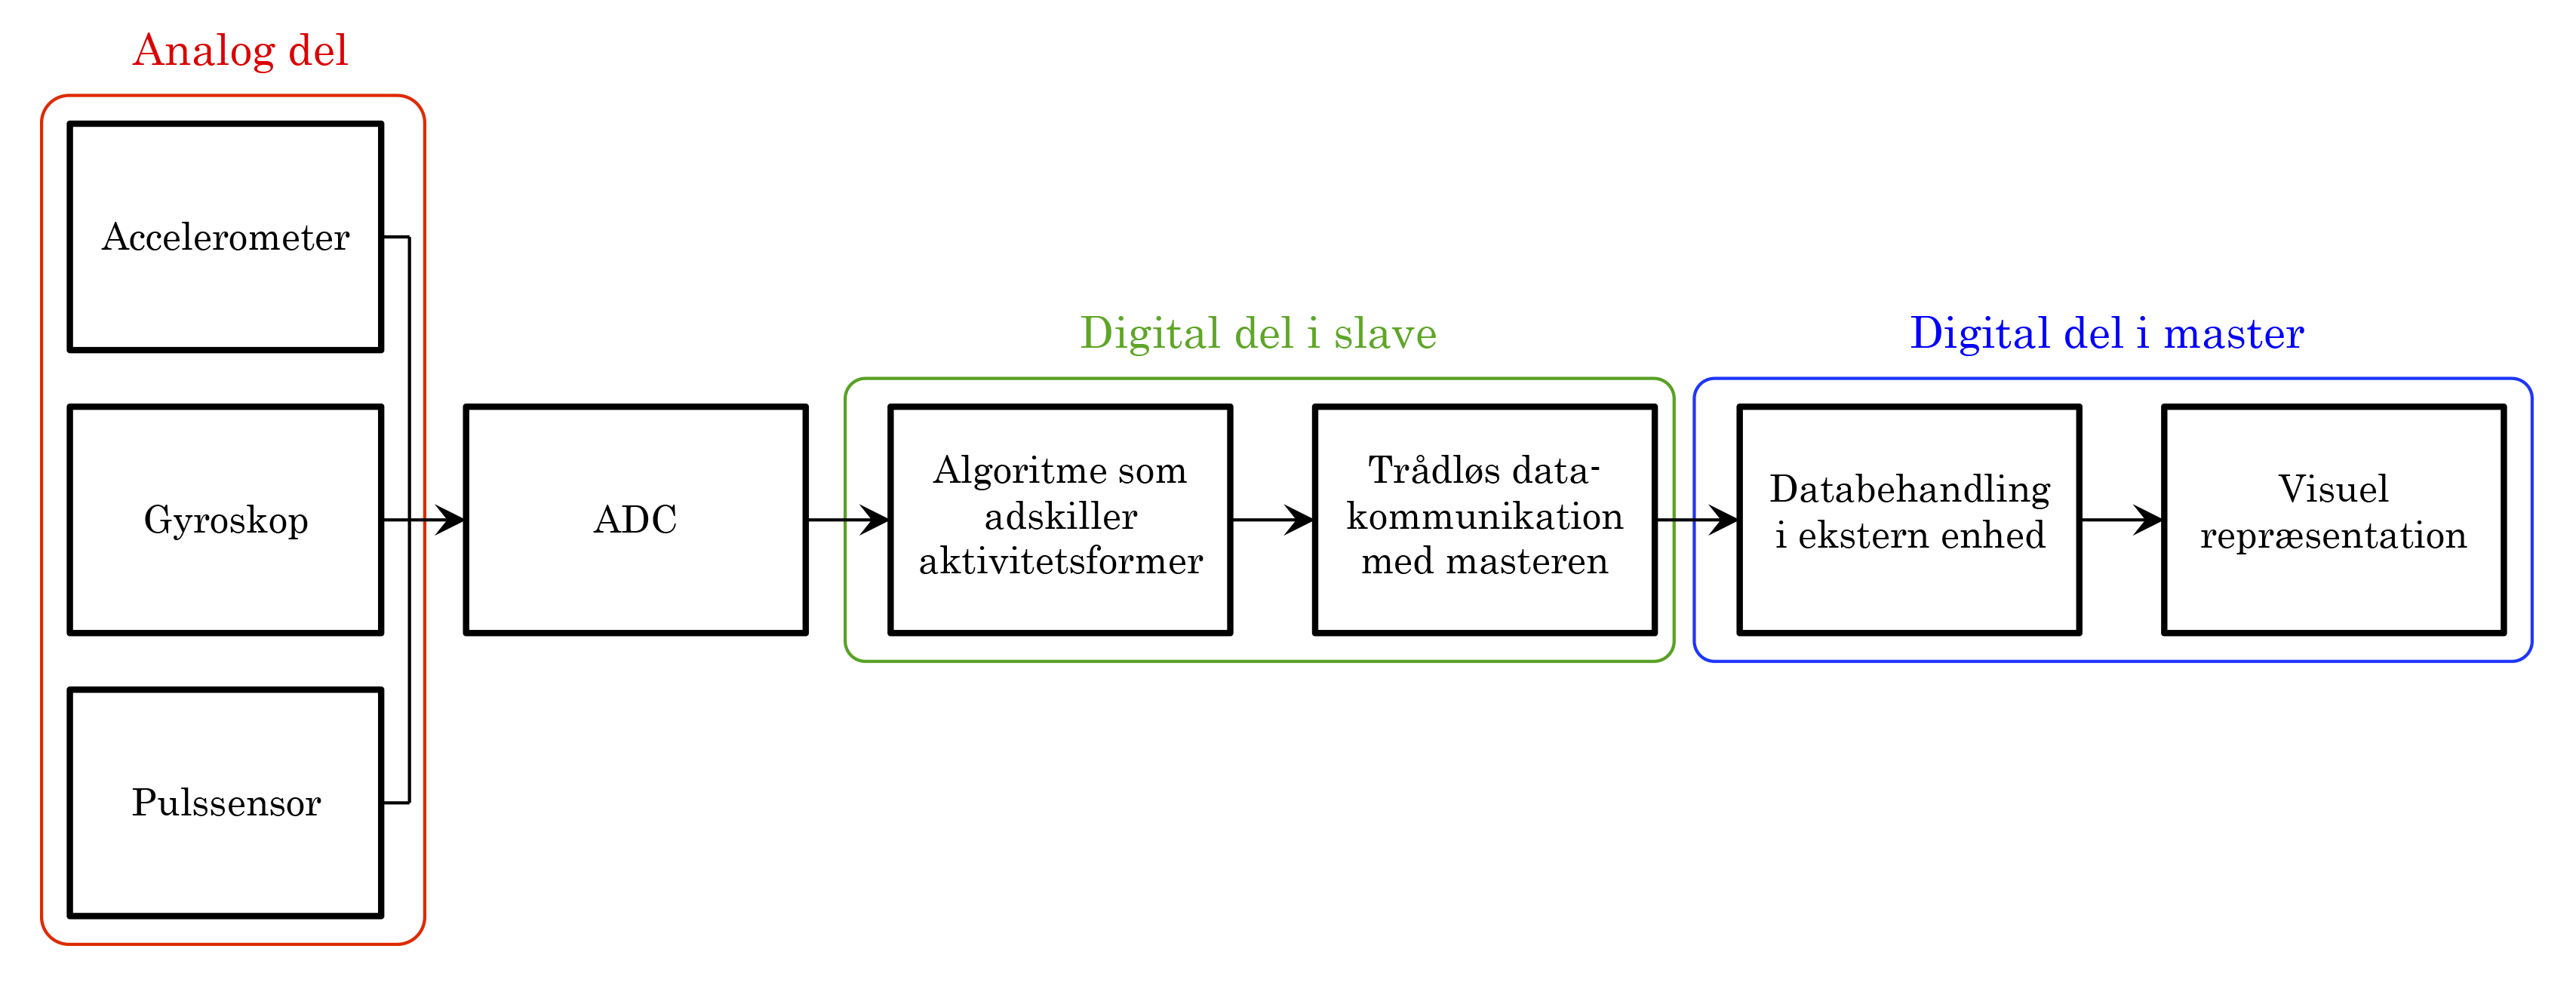
\includegraphics[scale=0.54]{figures/bProblemloesning/blokdiagram2.png}
 	\caption{Blokdiagram for systemet, som opdeles i den analoge del, og de to digitale dele. Den analoge del er omkranset med en rød firkant, slaven er omkranset med en grøn firkant og master er omkranset med en blå firkant.}
 	\label{fig:blokdiagram}
 \end{figure}
\section{Bevægelsesanalyse} \label{bevaegelse}
\textit{Følgende afsnit indeholder en bevægelsesanalyse af gang, løb og cykling. Dette udarbejdes med henblik på at finde karakteristika for de tre aktivitetsformer i forbindelse med detektering af aktiviteterne. Der vil derfor afslutningsvist være en sammenligning af karakteristika for de tre aktivitetsformer.}

\subsection{Gang}
Gang er en fysisk aktivitet, som er kendetegnet ved altid at have mindst en fod i jorden. Aktiviteten betegnes som en cyklus, der ses på \figref{fig:gang_cyklus}. Bevægelserne er identiske for højre og venstre ben men er forskudt med en halv cyklus i forhold til hinanden, hvorfor bevægelsen kun beskrives for højre ben.~\citep{VaughanDavisOConnor1992,Whittle1990} 
\begin{figure}[H]
	\centering
	\includegraphics[scale=0.7]{figures/bProblemloesning/gang_cyklus.png}
	\caption{På figuren ses en gangcyklus, som er illustreret for højre ben, opdelt i henholdsvis en standfase og en svingfase. Standfasen udgør en større procentdel af den samlede cyklus end svingfasen. Ydermere indeholder standfasen cyklussens hælnedslag og tåafsæt.~\citep{VaughanDavisOConnor1992} (Modificeret)}
	\label{fig:gang_cyklus}
\end{figure}\vspace{-0.25cm}
Følgende beskrivelse tager udgangspunkt i \figref{fig:gang_cyklus}. En gangcyklus inddeles i to faser: standfasen og svingfasen. Standfasens varighed er cirka 60\% af en gangcyklus og påbegyndes, når den højre hæl opnår kontakt med underlaget. Efter dette placeres foden fladt på underlaget, da venstre fod her hæves over jorden. Herefter opnår begge fødder kontakt med underlaget, mens der opstår et hælslip for den højre fod. Standfasen afsluttes med en dorsalfleksion af anklen og dermed et afsæt fra tæerne på højre fod.~\citep{VaughanDavisOConnor1992,Whittle1990}  \newline 
Når højre fod samt højre ben er i svingfasen, udgør dette cirka 40\% af en gangcyklus. Svingfasen påbegyndes med en acceleration af foden og benet, når foden ikke længere har kontakt med underlaget i standfasen. Den højre fod svinges fremad lige under kroppen. Afsluttende for svingfasen er der en deacceleration. Denne fase sænker hastigheden af benets og fodens fremadgående bevægelse. Derved er kroppen klar til det kommende hælnedslag, som initierer standfasen.\fxnote{herefter gentages cyklussen}~\citep{VaughanDavisOConnor1992,Whittle1990}

De to faser er dermed i retningerne af henholdsvis x- og y-aksen. \Figref{fig:kraefter_akser} viser kraftpåvirkningen på begge akser, som forekommer ved et hælnedslag.  
\begin{figure}[H]
	\centering
	\includegraphics[scale=0.55]{figures/bProblemloesning/kraefter_akser.png}
	\caption{På figuren ses kraftpåvirkningerne for x- og y-aksen ved et hælnedslag. Den resulterende kraft ved hælnedslag er indikeret med en grøn pil. Denne har en mindre vinkel til y-aksen, hvormed kraftpåvirkningen i y-aksens retning er størst.}
	\label{fig:kraefter_akser}
\end{figure}\vspace{-0.25cm} 
\Figref{fig:kraefter_akser} illustrerer den resulterende krafts retning i forbindelse med et hælnedslag. Yderligere fremgår det, at vinklen mellem den resulterende kraft og y-aksen er mindre end vinklen mellem x-aksen og den resulterende kraft. Kraftpåvirkningen i forbindelse med et hælnedslag er altså størst i y-aksens retning og derfor mest karakteristisk.~\citep{Rueterbories2010,Serway2010,ClelandKikhia2013}

\subsection{Løb}
Løb er en fysisk aktivitet, som er kendetegnet ved, at maksimalt én fod rører jorden af gangen. Aktiviteten er en hurtigere version af gang og beskrives ligeledes som en cyklus men indeholder fire faser, som det ses på \figref{fig:loebecyklus}: standfasen, den første svævefase, svingfasen og den anden svævefase. \citep{Adelaar1986,Novacheck1998}
\begin{figure}[H]
	\centering
	\includegraphics[scale=0.65]{figures/bProblemloesning/loeb_cyklus1.png}
	\caption{På figuren ses en løbecyklus opdelt i standfase, svingfase og to svævefaser. Standfasen udgør en større procentdel af cyklussen i forhold til svingfasen. Yderligere fremkommer svævefaser ved løb.~\citep{Adelaar1986} (Modificeret)}
	\label{fig:loebecyklus}
\end{figure}\vspace{-0.25cm}
Følgende beskrivelse tager udgangspunkt i \figref{fig:loebecyklus}. På samme vis som ved gangcyklussen begynder løbecyklussen, når højre hæl rammer jorden. Dette er begyndelsen af standfasen, som udgør 40\% af løbecyklussen. Herefter fortsætter foden til midtstand, hvor den er fladt placeret på jorden. Afslutningsvis udføres et accelererende afsæt med tæerne, som leder op til den næste fase, der er den første svævefase.~\citep{Adelaar1986,Novacheck1998} \newline 
De to svævefaser er identiske og udgør hver især 15\% af cyklussen. Disse er karakteriseret ved, at begge ben er løftet fra jorden. Svævefasen begynder idet, at tåafsættet har løftet foden fra jorden. Mellem de to svævefaser er svingfasen, som udgør 30\% af løbecyklussen. Denne fase indebærer, at højre fod og ben hæves og føres frem, hvorefter hælen igen isættes. Dette sker, mens den venstre fod udfører standfasen, hvorved højre fods svingfase er støttet af den venstre fod i jorden.~\citep{Adelaar1986,Novacheck1998} %Efter denne svævefase fase udføres anden svævefase før en ny cyklus kan påbegyndes. 

Ved løb er maksimalt én fod i kontakt med jorden ad gangen, hvilket resulterer i at der er et større stress på leddene ved løb i forhold til gang.~\citep{Adelaar1986} Dette suppleres af kraftpåvirkningen i de forskellige retninger under både gang og løb, hvor faserne domineres forskelligt af kraftpåvirkning i x- og y-aksens retning. \newline 
Standfasens hælnedslag og tåafsæt under gang og løb  er særligt karakteristisk grundet sin kraftpåvirkning i y-aksens retning. Kraftpåvirkningen er dog større ved løb, da denne fase ikke er understøttet af venstre fod. Kraftpåvirkningen i x-aksens retning for standfasen er af mindre betydning, da foden sættes i jorden og løftes op igen.\fxnote{Denne er større ved løb end gang, da hæl-nedslaget, som det ses på \figref{fig:loebecyklus}, er mere skråt på/har en mindre vinkel i forhold til jordoverfladen.} Modsat har svingfasen under gang og løb størst kraftpåvirkning i x-aksens retning, da accelerationen fremad af knæ og fod påvirker x-aksen mere end y-aksen.~\citep{Rueterbories2010} 
\subsection{Cykling}
Cykling er en aktivitetsform, der udnytter kraftoverførslen mellem en person og en cykel. For at opnå en fremdrift af cyklen benytter brugeren hovedsageligt en statisk position af overkroppen, hvorimod de nedre lemmer udfører kraftudviklingen.~\citep{Springer2014} Kraftoverførslen forekommer ved, at brugeren belaster cyklens pedaler. De roterende bevægelser med de nedre ekstremiteter skaber en fremdrift i hele systemet. Bevægelserne er opdelt i to lige lange faser; en kraftudøvende- og en restituerende fase, hvilket fremgår af \figref{fig:cykel_cyklus}.

\begin{figure}[H]
	\centering
	\includegraphics[scale=0.4]{figures/bProblemloesning/cykel_cyklus.png}
	\caption{På figuren ses cyklussen for cykling, som er opdelt to faser: en kraftudøvende- og en restituerende fase.~\citep{Springer2014} (Modificeret)}
	\label{fig:cykel_cyklus}
\end{figure}\vspace{-0.25cm}
Det fremgår af \figref{fig:cykel_cyklus}, at cykling er en bevægelse, som påvirker både x- og y-aksen. Der er dog tale om en cirkulær bevægelse om z-aksen. Idet cykling udføres i en cirkulær bevægelse, vil det være muligt at bestemme det antal grader, som benet har roteret om den pågældende akse. Derfor har en række studier beskrevet, at cykling med fordel kan detekteres af et gyroskop, som kan måle vinkelændringen af et bens bevægelse rundt om en akse. Dermed vil gyroskopets output for cykling være tilsvarende en sinussignal under ideelle forhold.~\citep{Cockcroft2011,Marin-PerianuMarin-Perianu2013} 

\subsection{Karakteristika for de tre aktivitetsformer}
En gangcyklus og løbecyklus er blandt andet karakteriseret ved at have en kraftpåvirkning i y-aksens retning ved hælnedslag og tåafsæt. Et eksempel på disse to kraftpåvirkninger i y-aksens retning kan ses under løb på \figref{fig:loeb_skolebog}. Signalet for gang vil til dels ligne dette signal dog med forskel på varigheden af henholdsvis stand- og svingfasen. Dette skyldes, at standfasen reduceres i varighed for løb i forhold til gang.
\begin{figure}[H]
	\centering
	\includegraphics[scale=0.45]{figures/bProblemloesning/loeb_skolebog.png}
	\caption{På figuren ses et signal for løb optaget med et accelerometer, der er placeret på anklen. Accelerationen på y-aksen fremgår som funktion af tiden på x-aksen. En cyklus er angivet med den tilhørende stand- og svingfase, hvoraf de to svævefaser indgår i svingfasen. Ydermere er hælnedslag markeret med et blåt kryds, og et tåafsæt er markeret med en gul cirkel.~\citep{Strohrmann2011} (Modificeret)}
	\label{fig:loeb_skolebog}
\end{figure}\vspace{-0.25cm}
En cykelcyklus har ikke nogen væsentlig acceleration i vertikal eller horisontal retning men derimod rotation om en akse. Måling med et gyroskop vil dermed repræsentere ændringerne i vinklen om aksen.~\citep{Cockcroft2011,Marin-PerianuMarin-Perianu2013} 

\section{Brugersikkerhed}
\textit{Nedenstående afsnit beskriver hvilke ricisi der kan forekomme når en bruger tilkobles elektronisk udstyr. Metoder hvorpå de omtalte risici kan forebygges, beskrives også. Afsnittet underbygges af det funktionelle krav, hermed at systemet skal været sikkert for brugeren at anvende.}

Medikoteknisk udstyr er tilsluttet en spændingsforsyning i form af eksempelvis strømnettet eller et batteri. Der indgår derfor en spænding og dermed en elektrisk strøm i det elektroniske kredsløb. En elektrisk fare kan opstå når brugeren er tilkoblet det medikotekniske udstyr, og kan dermed risikere at blive udsat for makro- og mikroshock fra hele det elektriske kredsløb. Makroshock er defineret som en elektrisk strøm, som løber igennem kroppen på den tilsluttede person. Denne strøm løber oven på huden, og er overfladisk. Mikroshock er defineret som elektrisk strøm, som løber igennem en persons væv deriblandt hjertet. Den elektriske strøm som personen påvirkes med under mikroshock, medfører oftest en større potentiel fare end makroshock. Eksempelvis kan makroshock forårsage mindre muskelkontraktioner og er ofte ikke-dødelige skader. Derimod kan mirkoshock være store vævsskader samt dødelige elektriske påvirkninger af personen. \citep{Webster2011} \newline
Medikoteknisk udstyr har dermed en risiko for at påføre brugeren en strøm som potentielt kan være farlig. Det er derfor væsentligt, at det elektroniske udstyr involverer sikkerhedsmæssige elementer således risikoen for lækstrømme sænkes. Eksempelvis benyttes isolation og jordning som sikkerhedsmæssige procedurer, for at nedbringe risikoen for at tilføre brugeren lækstrømme i form af henholdsvis makroshock eller mikroshock. Isolation benyttes til at isolere brugeren fra elektriske spændingskilder i det medikotekniske udstyr. Ydermere benyttes jording som en sikkerhedsforanstaltning, idet alle aktive komponenter føres til jord, altså et fælles nulpunkt. De aktive komponenter er forbundet til jord, hvormed eventuelle lækstrømme vil løbe denne vej og dermed væk fra brugeren. \citep{Webster2011} \newline 
Systemet skal være mobilt som det fremgår af \secref{succeskrav}. Systemet vil dermed have en spændingsforsyning i form af et knapcelle batteri, hvilket vil tilføre en lav spænding. Benyttelsen af batterier kan dog være forbundet med enkelte, mindre sikkerhedsmæssige farer. Farerne kan opstå hvis batterierne ikke bliver brugt efter de foreskrevne regler for det pågældende batteri. Dette kan risikere at ødelægge batteriet, hvormed brugeren vil kunne blive udsat for forbrændinger som følge af fejlbrug af batteriet. Et ødelagt batteri kan ydermere risikere at medføre åndedrætsbesvær for brugeren. Disse farer kan undgås hvis man følger batteriets sikkerhedsanvisninger. \citep{NREL2011}


%  For at sikre lækstrømme ikke opnår en størrelse hvormed makro- og mikroshock kan være alvorligt skadelige, kan isolation benyttes. Ved isolation sikre man at det medikotekniske udstyr ikke er i direkte forbindelse med en betydelig spændingskilde. I og med at udstyret er forsynet med en lav spændingskilde, begrænses størrelsen af de lækstrømme som kan forekomme. Den anden sikkerhedsforanstaltning som kan implementeres for at gøre udstyret sikkert for brugeren er jording. Jording sikre at alle
\section{Analog teori}
\textit{Følgende afsnit omhandler de teoretiske aspekter af systemets hardware. Blandt andet beskrives systemets sensorerne, accelerometer og gyroskop. Disse sensorer beskrives med henblik på at kunne kan detektere de ønskede aktiviteter. Sensorerne beskrives overordnet for at danne en forståelse for deres virkemåde og hvordan disse kan udnyttes.}

\subsection{Accelerometer}
Et accelerometer er et elektromekanisk apparat, som anvendes til at måle accelerationskræfter, hvilket er ændringer i hastighed og position \citep{Goodrich2013,TittertonWeston2004}. Enheden for dette er $m/s^2$ og $g$, hvor 1 g svarer til 9,82$m/s^2$. Et accelerometer måler dermed egenaccelerationen af et givent objekt. \fxnote{En g-kraft på jorden svarer til tyngdekraften på 9,82$m/s^2$, men varierer med elevation. Wiki har en god forklaring af dette, hvis man stadig er i tvivl.}\citep{Sparkfun,TittertonWeston2004} \newline

Et accelerometer måler to former for acceleration, henholdsvis statisk og dynamisk. De statiske kræfter er tyngdekraften med henhold til vinkelretningen af accelerometeret. De dynamiske kræfter beskriver retningen af accelerometerets bevægelse og dets vibrationer. \citep{Sparkfun,Goodrich2013,Engineering}. Ydermere forefindes accelerometre med henholdvis en, to eller tre måleakser.  \citep{TittertonWeston2004} 

Accelerationen i et accelerometer beregnes ud fra Newtons anden lov, $F=ma=mf+mg$, hvor den totale kraft (F), er lig med den påvirkede masse (m), ganget med dets acceleration (a). Dette kan også defineres som massen (m) multipliceret med henholdsvis de eksterne kræfter (f) og tyngdekræften (g). \citep{TittertonWeston2004,Academic2016d} \newline
Illustrativt kan et accelerometer beskrives som en kapsel, hvori der er en indre masse spændt mellem to fjedre, hvilket illustreres på \figref{acc_simpelt}. Ændringen af den indre masse i den sensitive akse kan dermed beskrive accelerationen af selve accelerometeret i den pågældende akse. Hvis accelerometeret kastes op i luften, vil både kapslen og den indre masse udelukkende påvirkes af tyngdekræften, og der vil derfor ikke registeres en acceleration.\citep{TittertonWeston2004,Academic2016d} \newline

\begin{figure}[H]
	\centering
	\includegraphics[scale=0.5]{figures/bProblemloesning/accelerometer_basic.png}
	\caption{På figuren fremgår opbygningen af et accelerometer med en indre masse, fjedre og den ydre kapsel. Det ses på den indre masse, at denne er forskubbet mod bunden af kapslen, grundet en acceleration af accelerometeret. \citep{TittertonWeston2004} (Modificeret)}
	\label{acc_simpelt}
\end{figure}
Ethvert stillestående objekt påvirkes af +1 g i den positive, vertikale akse \citep{Serway2010}. Derfor vil et stillestående accelerometer altid påvirkes af $\pm$1g på én bestemt akse afhængig af sensorens orientering. Eksempelvis, hvis accelerometeret er placeret på et bord med dets positive y-akse i vertikal retning, da vil y-aksen blive påvirket med $+$1 g. I dette tilfælde vil de andre akser, henholdsvis x-, og z-aksen, ikke blive påvirket af nogen kræfter, med antagelse om idelle betingelser. 

Accelerometre benyttes enten i en åben eller lukket kreds. I en åben kreds fastholdes den indre masse til et nulpunkt ved at være udspændt mellem to fjedre. Ved acceleration af den ydre kapsel bevæges den indre masse væk fra nulpunktet, hvorved ændringen for et single-akse accelerometer vil være proportional med kræften, som påvirker systemet. \newline
I en lukket kreds fastholdes den indre masse til et nulpunkt ved hjælp af magnetiske kræfter. Oftest påmonteres en spole på den indre masse, hvormed magnetfeltet forstærkes. Det er muligt at foretage mere præcise målinger omkring nulpunktet end ved ændringerne. Accelerometre med den lukkede kreds er derfor mere præcis, end accelerometre med en åben kreds. \citep{TittertonWeston2004,Academic2016d,Serway2010}

\subsection{Gyroskop}
Et gyroskop er et elektromekanisk apparat, som anvendes til at måle omdrejninger per sekund eller vinkelhastighed om en given akse, hvilket illustreres på \figref{fig:gyro}. Enhederne på data fra et gyroskop er henholdsvis revolutions per second (RPS) og $^\circ$/sekund. \newline
Et gyropskop kan give information om orienteringen eller navigationen af objektet, som sensoren optager data fra. Hvis et gyroskop eksempelvis drejes én omgang om egen akse i sekundet, vil den registrere en vinkelhastighed på 360 grader pr sekund. \citep{Sparkfun_gyro,Barbour2014}
\begin{figure}[H]
	\centering
	\includegraphics[scale=0.6]{figures/bProblemloesning/gyro.png}
	\caption{På figuren ses et gyroskops måling af rotation omkring x-, y- og z-aksen. \citep{Sparkfun_gyro} (Modificeret)}
	\label{fig:gyro}
\end{figure}

Alt afhængigt af formålet med at benyttes et gyroskop, findes der en række forskellige gyroskoper heriblandt vibrations-, elektrostatiske- og kernemagnetisk resonans gyroskoper. \citep{LuingeVeltink2005,TittertonWeston2004} Et gyroskop kan for eksempel registrere vinkelhastighed ved at anvende tyngdekræften og en lille indre masse \citep{Sparkfun_gyro,Barbour2014}. Hvis et gyroskop eksempelvis opsamler data ved cykling, mens det er placeret proximalt for den laterale malleolus, vil massen blive udsat for en roterende bevægelse omkring den horisontale akse. Massen vil blive henholdsvis tungere og lettere i processen på grund af ydre påvirkende kræfter, hvorfor outputtet vil komme til udtryk som en sinus-bølge. Outputtet er afhængig af tyngdekræftens påvirkning af massen, hvorfor et varierende output kræver en bevægelse.% Gyroskopet vil, uafhængigt af placering, have et fast output, som det vil vende tilbage til efter en bevægelse.
%Et gyroskop fungere ved at anvende inerti egenskaberne der opstår når et hjul spindes med en høj hastighed. Ved at hjulet fastholder den samme retning omkring aksen, kan impulsmomentmomentet, dets inertiprodukt samt hastighed være med til at definere en referenceretning. 
%De fundementale principper bag virkningen af et gyroskop er blandt andet det gyroskopiske inerti, som er når hjulet drejer om sin egen akse og står vinkelret på aksen. impulsmomentet som er fordelingen af en masse på et rotor, hvor vinkelhastigheden også har en betydning, og præcession som er rotationen omkring egen akse. 
%De signaler som opfanges af et accelerometrer, inkluderer ikke signaler fra den roterende akse og derfor kan en præcis orientering ikke opfanges. For at forbedre nøjagtigheden, kan man anvende gyroskoper som et supplement til accelerometre .
%Et gyroskop måler vinkelhastighed, hvor ændringen i orientering kan måles ved at integrere vinkelhastigheden på baggrund af en algoritme. \citep{LuingeVeltink2005}
%
\subsection{Sammenligning af accelerometer og gyroskop}
Et acceleromteter er i stand til at måle accelerationen af et objekt, eksempelvis bevægelsen af et ben under gang og løb. Dette er muligt da denne sensor måler den kraft som eksempelvis et ben påvirkes med, ved en given bevægelse. Denne kraft vil medføre karakteristiske udsving for den givne bevægele. Særligt gang og løb har en karakteristisk påvirkning på kroppen vedrørende acceleration. Accelerometeret vil derfor være fordelagtigt at benytte til en registrering af gang og løb, da det er muligt at genkende og bestemme betydningen af disse karakteristika. Gyroskopet registrerer rotationen af et objekt om en given akse. Med antagelse om ideelle forhold vil det derfor være fordelagtigt at benytte et gyroskop til registrering af cykling, idet denne bevægelse overordnet set er en cirkulær bevægelse omkring én akse. Betydningen heraf. vil medføre at cykling tilnærmelsesvis kan afspejles som en sinus bølge med varierende frekvens alt efter hastighed. 

%\textbf{Gammelt forslag} \newline
%Den væsentligste forskel er, at et gyroskop kan måle rotation, hvilket et accelerometer ikke er i stand til. Accelerometret er fordelagtigt at bruge til at måle orientering af et stationært punkt i forhold til jordens overflade men under bevægelse bliver outputtet mere komplekst. For eksempel vil et accelerometer under frit fald vise 0. \citep{Goodrich2013,TittertonWeston2004,LuingeVeltink2005} \\
%Et gyroskop reagerer ikke på vibration eller støj, hvilket et accelerometer kan opsamle som støj på signalet. Derudover reagerer et gyroskop hurtigt men dets output for hældningsvinkel vil blive mere ukorrekt over tid grundet usikkerhed i de enkelte målinger, hvorfor den akkumulerede vinkel ligeledes bliver mere ukorrekt. Et accelerometers respons er langsommere men mere præcis over tid. Igennem kalibrering, hvor hvert apparat assisterer til kalibreringen af den anden, vil de tilsammen kunne holdes korrekt på kort og lang sigt. \citep{Barbour2014,Brasca2011}
\subsection{Pulssensorer}
Kroppens puls kan detekteres på en række forskellige måder, eksempelvis elektrisk eller optisk.
Elektriske pulssensorer, måler pulsen ved hjælp af en elektrisk kontaktflade mellem sensor og person, hvilket skabes ved hjælp af elektroder. Pulsen detekteres af de elektriske pulssensorer, som forskelle i den elektriske ladning. Udfaldet af målingerne kan være afvigende, da individuelle faktorer såsom en personens blod, svedniveau eller hudfedt er en afgørende faktor. For at minimere disse udfald kræves der en god elektronisk kontakt, heraf er præparering af huden nødvendig. Denne type plusmåling kræver en placering ved hjertets afledninger\fxnote{https://www.sundhed.dk/borger/sygdomme-a-aa/hjerte-og-blodkar/illustrationer/tegning/placering-af-ekg-elektroder/}. \citep{PhuaLissorguesMercier2009}  \\
Optiske pulssensorer registrerer puls ved hjælp af lysindhold. En LED udsender en lyskilde som passerer huden og blodåren, hvoraf en mængde af dette lys absorberes af hæmoglobin i blodet. Efterfulgt af dette opfanger en fotodiode mængden af det resterende lys. Størrelsen af dette lys er den bestemmende faktor vedrørende mængde blod i blodåren, og er heraf omvendt proportionalt. Pulssensoreren udsender positive udsalg på signalet, desto mere blod der registreres. Denne type sensor bruges ofte i fingerspidsen eller på tåen.\citep{PhuaLissorguesMercier2009,SrinivasReddySrinivas2006} 

%\subsubsection{Registrering af puls}
%Pulsen er angivet som forskellen i det systoliske og diastoliske blodtryk som slag per minut. Pulsen kan måles manuelt ved at placere to fingre over en arterie, og derefter tælle hvor mange slag der er i minuttet. Hyppigst måles pulsen fra radial arterien på håndleddet eller på halsen, men enhver arterie der kan mærkes, kan bruges til at måle pulsen ved, se \figref{pulsmaaling}. \citep{CNX2016}
%
%\begin{figure}[H]
%	\centering
%	\includegraphics[scale=0.6]{figures/bProblemloesning/puls.png}
%	\caption{På figuren ses steder det er muligt at måle puls.\citep{CNX2016}}
%	\label{fig:sensor_placering}
%	\end{figure}
	



\section{Digital Teori}
\textit{Noget om denne section?}

\subsection{CY8CKIT-043 PSoC 4-M og PSOC Creater}
Til dette projekt anvendes CY8CKIT-043 Programmable System on Chip (PSoC) 4 M-Series Prototyping Kit og programmet PSoC Creater i den digitale del til at opsamle det biologiske signal.\\
CY8CKIT-043 PSoC 4 M-Series Prototyping Kit er en prototyping platform, der indeholder tre mikroprocessorer: to Programmable System-on-Chips (PSoC) og en Programmable Radio on Chip (PRoC), hvilket ses på \figref{fig:PSoC}. Den første PSoC LP5 på mikrokontrolleren sidder på KitProg boardet og kan indeholde programmer, der kan indlæses på en computer ved hjælp af USB stikket. Den bruges til at programmere og debug softwaren på target boardet af mikrokontrolleren, hvorfor denne del kan knækkes af resten af stikket og fungere selvstændigt. Dette kræver dog, at softwaren først er programmeret på den anden mikroprocessorer, som er PSoC 4200M. Denne fungerer som hovedcomputeren, der programmeres på igennem c koden, og muliggøre eksempelvis høj-performans analog til digital konvertering igennem sin 12-bits SAR ADC. På bagsiden af mikrokontrolleren sidder en PRoC med Bluetooth Low Energy(BLE). Denne PRoC har ikke lige så mange muligheder for afbenyttelse i forhold til PRoC 4200M, da BLE optager meget plads, hvorfor der ikke er plads til meget andet. \citep{CYPRESS2016PSoC,Semiconductor2016,CYPRESS2016Cortexm0}
\begin{figure}[H]
	\centering
	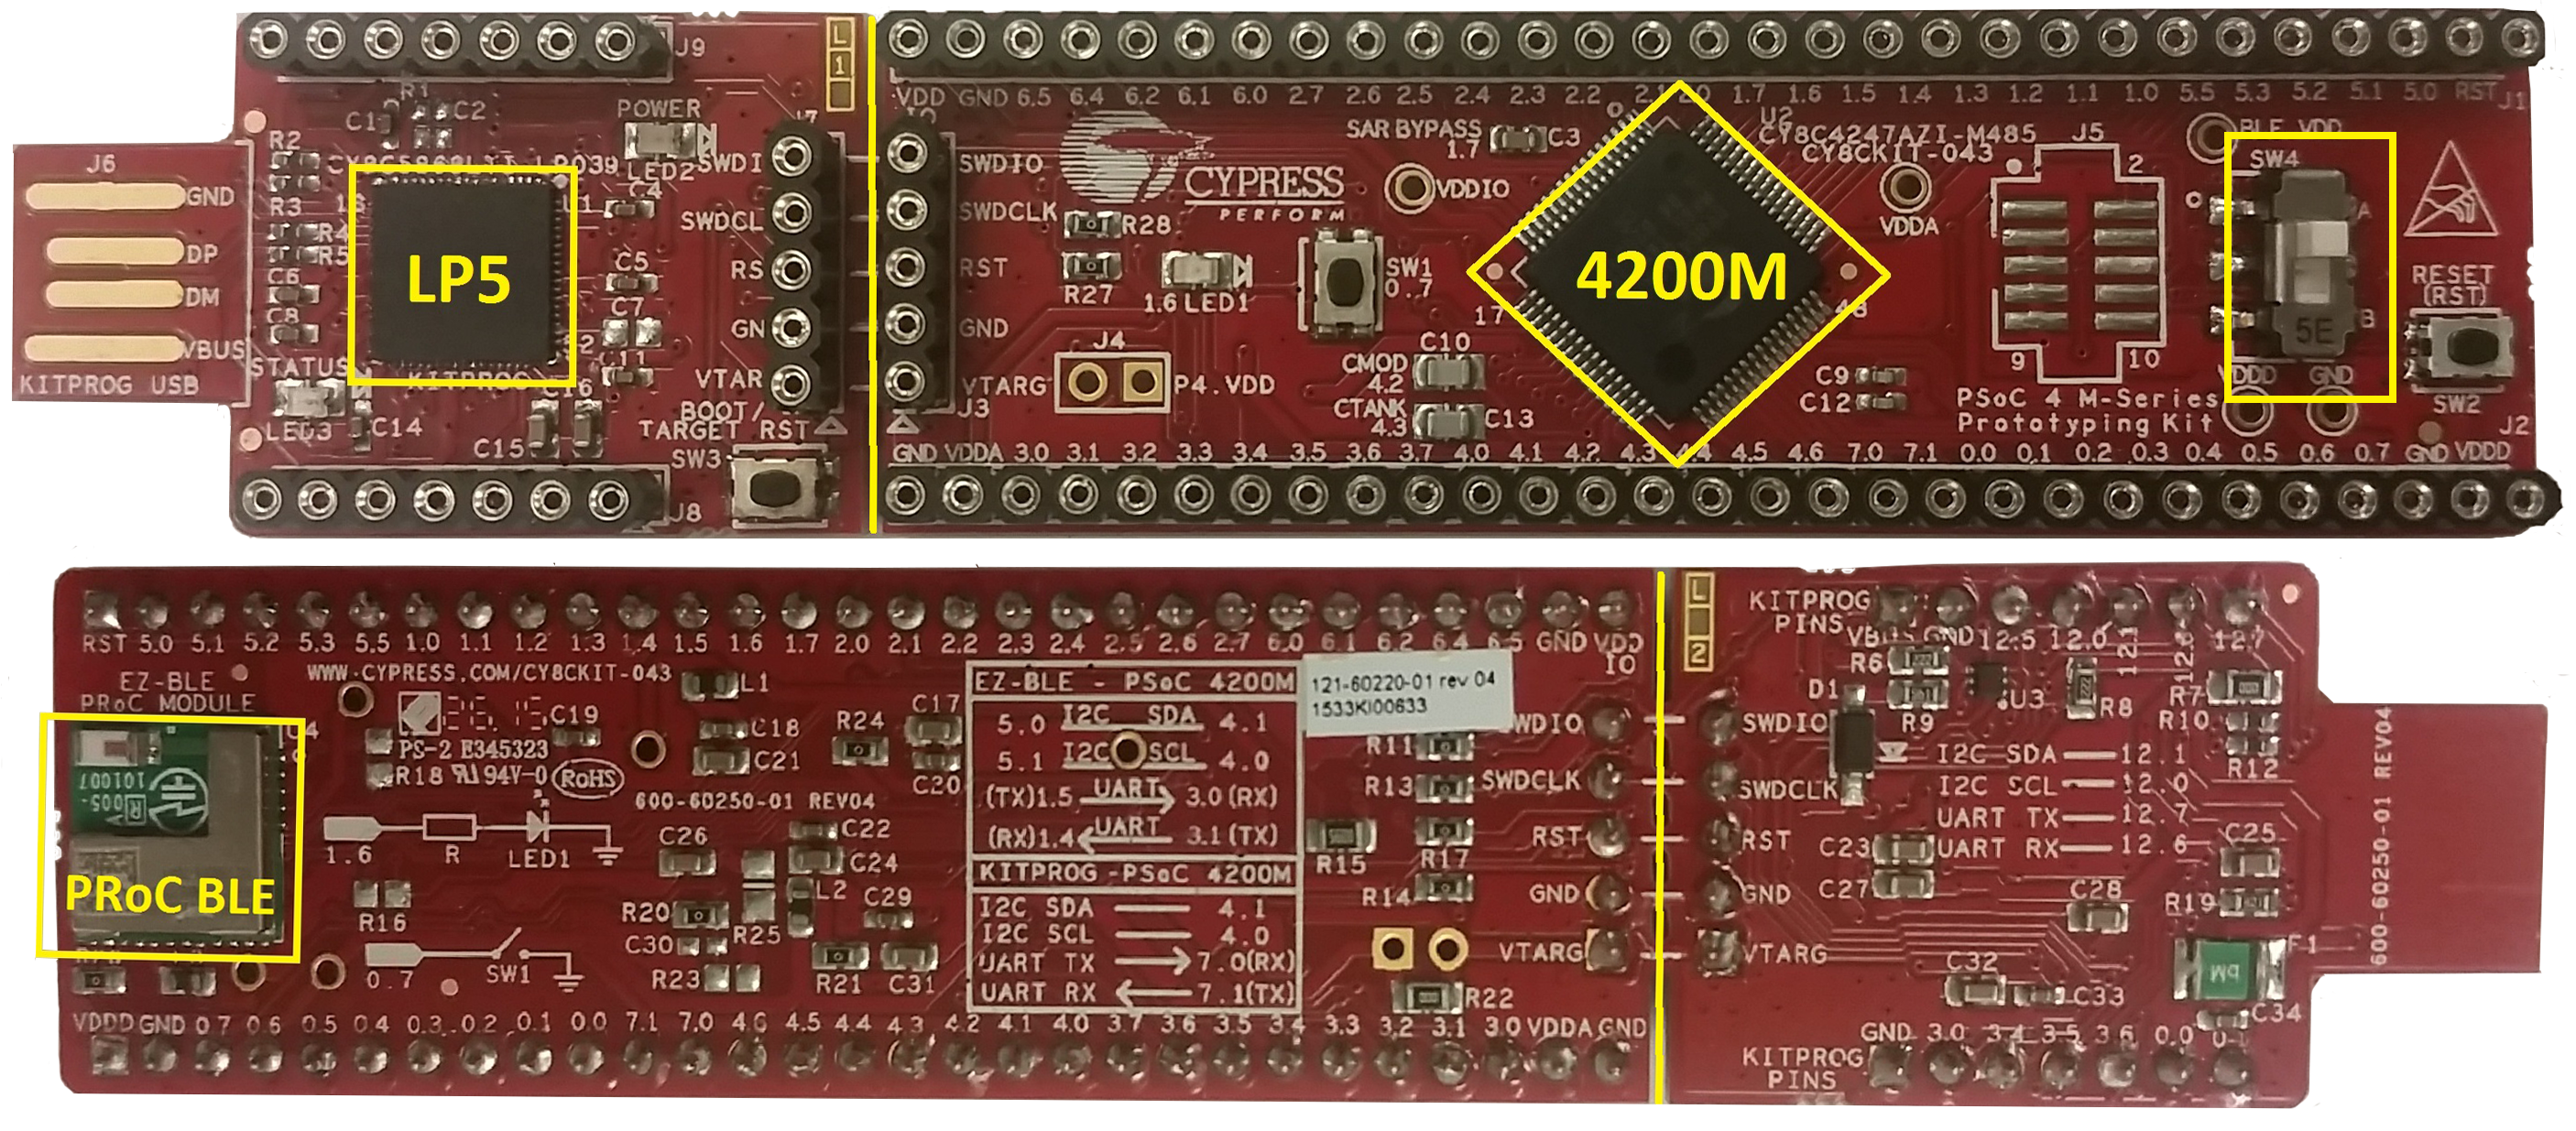
\includegraphics[scale=0.15]{figures/bProblemloesning/PSoC3.jpg}
	\caption{På figuren ses mikrokontrolleren CY8CKIT-043 PSoC 4 M-Series Prototyping Kit foran og bagpå. På forsiden findes to PSoC og på bagsiden findes PRoC, som alle er tydeliggjort med gul markering og navngivning. Mikrokontrolleren kan knækkes over i to: KipProg board med USB stik og target board med hovedchippen PSoC 4200M\fxnote{Navnene er fundet nederst på side 26 i manualen}. PRoC'en er ikke påmonteret som standart fra Cypress, hvorfor denne er blevet loddet manuelt på efterfølgende. Kontakten helt til højre på forsiden af target boardet, som også er loddet manuelt på efterfølgende, skal trykkes ned for, at PRoC programmeres på istedet for PSoC 4200M. \citep{CYPRESS2016PSoC,Semiconductor2016}}
	\label{fig:PSoC}
\end{figure}
Når data skal opsamles, skal to CY8CKIT-043 PSoC 4 M-Series Prototyping Kit benyttes. Én skal placeres på personen og opsamle data, som skal sendes til en anden mikrokontroller, der er koblet til en computer via USB. Dette kan lade sig gøre, da mikrokontrolleren har Inter-Integrated Circuit (I$^{2}$C) interface. I$^{2}$C er en computerbus dataprotokol, hvilket gør det muligt for de to mikrokontrollere at opføre sig som master eller slave. Rollen i kredsen bestemmes igennem softwaren. Masteren kontrollerer I$^{2}$C bussen og sender kommandoer til slaven. Både master og slave kan sende og modtage data, men masteren kontrollerer, hvornår dette kan finde sted. Det er muligt med I$^{2}$C interface at lave flere slaver eller flere masters til slaverne. I dette tilfælde vil der være én slave og én master. Disse kan kommunikere ved hjælp af et virtuelt kabel, som skabes af BLE. \citep{Semiconductor2016,Sparkfun2016}\\
Mellem PSoC LP5 og PSoC 4200M samt mellem PSoC 4200M og PRoC findes blandt andet nogle serielle porte med to ledninger til at modtage data (RX) og sende data (TX). Disse tre mikroprocessorer kommunikerer altså ikke på samme måde, som to mikrokontrollere kommunikerer med hinanden. \citep{Semiconductor2016} \\
Mikrokontrolleren kræver en ekstern strømkilde for at kunne fungere. Igennem USB porten adapteres tilslutningen til 5V, men det er muligt at tilkoble en strømkilde til boardets lav-volt applikation, hvilket gør den trådløs. 3,3V til 5,5V tilsluttes VDD fra en reguleret forsyning, hvilket er yderst essentielt, da boardet ikke besidder en elektrostatisk afladnings beskyttelse (ESD). Hvis en ekstern strømforsyning til VDD er for ustabil eller af dårlig kvalitet, kan mikrokontrollerens kredsløb blive forstyrret og vil derved ikke fungere optimalt. \citep{Semiconductor2016}

Programmet PSoC Creater kan designe hardware og software til mikrokontrolleren. Herigennem bliver rekonfigurerbare analoge blokke og digital programmerbar logik kombineret\fxnote{kan den fysiske hardware opbygges digitalt}, hvorved softwaren kan tilpasses de fysiske komponenter direkte igennem kodedesign. Programmet indeholder forskellige komponenter og kodeeksempler, hvilket kan blive behjælpeligt under algoritmedesignet. \citep{Semiconductor2016} \\
Når mikrokontrolleren er tilsluttet computeren og debugger igennem PSoC Creater, kan matlab fungere som et grafisk bruger interface (GUI). Dette muliggør live visualisering af den data, som eksempelvis en master mikrokontroller modtager fra en slave mikrokontroller.

\subsection{Mikrokontrollerens target CPU}
Target CPU'en på CY8CKIT-043 PSoC 4 M-Series Prototyping Kit er 4200M, som besidder en ARM cortex-M0 processer og har produktnavnet CY8C4247AZI-M485. Denne er basseret på Instruction set architecture (ISA) kategorien Reduced Instruction Set Computer (RISC). ISA beskriver\fxnote{processor design teknikken}, hvordan processoren vil bearbejde dens instruktioner. ISA's kategorier kan blandt andet være complex instrucion set computer (CISC) eller RISC. En CISC baseret computer vil udføre opgaver med så få linjer som muligt. Processorens hardware opbygget til at forstå og udføre komplekse instruktioner, hvilket kræver flere transistorer end RISC metoden. RISC processorer benytter simple instruktioner, som kan forløbe inden for en clock cycle\fxnote{dansk? I så fald klok omgang?}. Derimod kræver dette mere RAM, fordi hver opgave hentes ned og gemmes indtil færdiggjort. Denne metode tillader dog pipelinning, hvilket gør at flere instruktioner kan køre samtidig.\fxnote{fetch - decode - exicute. Mere laves samtidig} Sammenlignet er RISC processen hurtigere end CISC, men CISC computere kan udføre flere komplekse instruktioner på færre linjer end RISC. \citep{CYPRESS2016Cortexm0,Semiconductor20164200M,Yadav2016}\\
CPU'en i Cortex-M0 er en del af det 32-bit microcontroller unit (MCU) delsystem, som optimerer energibesparende drift ved hjælp af clock gating\fxnote{Clock gating saves power by adding more logic to a circuit to prune the clock tree. Pruning the clock disables portions of the circuitry so that the flip-flops in them do not have to switch states. Switching states consumes power. When not being switched, the switching power consumption goes to zero, and only leakage currents are incurred}. %% Noget om deep sleep / low power mode (Hvis den har det), hvor mange registre den har og hvis nogen af dem har dedikerede funktioner
CPU'en har en flash hukommelse på 128 kB og en 16 kB RAM. Algoritmen og dermed programmet for mikrokontrolleren gemmes i flash, da RAM hukommelsen kræver konstant strøm og slettes dermed, hvis strømtilførslen til mikrokontrolleren slukkes. \citep{Semiconductor20164200M}

tilgængelige pins - tilkobling af perifære moduler, som f.eks. en sensor
Mere om ADC'en 12-bits SAR ADC med 1 mega sample pr sekund (Msps) konverterings rate. (se end tial forcing - biofeedback til apopleksi). men ADC virker ikke under deep sleet mode, fordi den kræver høj hastighed clock
oscillatorer - styrer hastigheden på clocks, afhænger af spændingsfrosyning, men der er en 32 kHz (ILO Clock) low power mode (forklar om dette, meget relevant)
output - (se end tial forcing)

\subsection{Interrupts}
Interrupt er en funktion, som kan afbryde main filen for CPU'en, hvis en bestemt hændelse sker eller  - Detektion af diafragma \citep{Badiger2016}

%%%%%%%%%% Clocks
- detektion af diafragma, spilbaseret

%%%%%%%%%% Trådløs kommunikation - Bluetooth
radiomoduler - (Aktivitetsmåler til monitorering)

UART (Aktivitetsmåler til monitorering)



%
%
% I pdf'en for mikrokontrolleren - se side 23
% Skrive om I2C
%
%Denne prototyping Kit platform er ved hjælp af en computer med aktiv bluetooth i stand til at sende og modtage trådløs data fra Y8CKIT-042-BLE Bluetooth® Low Energy (BLE) Pioneer Kit platformen, som indeholder en PRoC.
%CYPRESS2016BLE
%CYPRESS2016PSoC
%Semiconductor2016
%Semiconductor2016BLE
\subsection{Universal Asynchronous Receiver Transmitter(UART)}
En UART er et led mellem et parallelt og serielt interface, der både modtager data(RX) og sender data(TX). Dataen sendes som bit, og kan både sendes serielt eller parallelt.\newline 
Parallelt bliver flere bit overført på samme tid, hvormed et 8-bit system er nødsaget til at have 8 ledninger, hvor der i den ene ende er en RX kobling og den anden er TX kobling.\newline
Den serielle kommunikation foregår asynkront, og kan foregå med en ledning, da kun en bit overføres af gangen. Oftest benyttes den serielle kommunikation, da denne ikke kræver så mange ledninger.  Det er nødvendigt at sætte en baudrate, da TX sender i forhold til denne og RX sampler i forhold til den forventede baudrate\fxnote{baudrate = Hvor hurtigt der sendes data (bits per sekund[bps])}. Det modtagne data gemmes ofte i en buffer, som efterfølgende videregives i form af firs-in-first-out (FIFO) princippet.\newline 
Overførsel af data sker asynkront, som det ses på \figref{fig:asynkron}. Ved denne kommunikationsform opererer RX og TX ved to forskellige klokker. For at kunne lave dataen synkront, sættes der et startbit og et stopbit. UARTens opgave er at læse data fra FIFO parallel data, som så laves om til seriel data Dette data kan så sendes til andre enheder. Når RX i en anden enhed modtager et startbit, laves data om fra seriel til parallel data, hvorefter data kan skrives til modtager-FIFO. 

\begin{figure}[H]
	\centering
	\includegraphics[scale=0.6]{figures/bProblemloesning/asynkron.png}
	\caption{På figuren ses asynkron dataoverførsel.\citep{Jimb02016}}
	\label{fig:asynkron}
\end{figure}

Nogle enheder indeholder mere end en seriel-linje, og disse enheder fungerer enten som fuld-duplex eller halv-duplex. De enheder der er fuld-duplex, kan både sende og modtage data på samme tid. Ved halv-duplex, skal dette foregå på skift. 
\input{rapportAfsnit/dProblemloesning/Power_mode}
\subsection{Digitale filtre}
% IIR 
% FIR
% Moving average
% threathold 


Et filter har typisk til formål at frafiltrere uønskede frekvenser fra signalet\fxnote{opg: andre formål}. Ønskes det at fjerne høje frekvenser, anvendes et lavpasfilter, som lader frekvenser under en valgt værdi passere, mens der, hvis man ønsker de lave frekvenser fjernet, anvendes et højpasfilter, som lader de høje frekvenser over en valgt værdi passere. Disse to filtertyper kan kombineres alt efter om man vil fjerne frekvenser udenfor et bestemt spektrum, båndpasfilter, eller kun vil fjerne en lille del af spektret, båndstopfilter, hvilket er illustreret på \figref{fig:filtre}\fxnote{opg: skal figuren være der?}. Ved en sammensætning hvor lavpasfilteret dæmper efter højpasfilteret, og højpasfilteret dæmper før lavpasfilteret, fås et båndpasfilter. Sammensættes de to filtre modsat med et lavpasfilter som dæmper før højpasfilteret mens højpasfilteret efter lavpasfilteret, fås et båndstopfilter.
\citep{Ramsden2001}

\begin{figure}[H]
	\centering
	\includegraphics[scale=0.2]{figures/bProblemloesning/filtre.png}
	\caption{På figuren ses ... \citep{Aasvik2016} (Modificeret)}
	\label{fig:filtre}
\end{figure}

FILTERTYPER

Infinite impulse response (IIR)
- Butterworth
- chebyshev 
- ect. 
Finite impulse response (FIR)
- Parks-McClellan algorithm
- Frequency sampling
- window type
- ??

\subsubsection{Filterdesign}
I designfasen for filtre, startes der med at blive set på signalets frekvensspektrum, hvorved det vælges om der er behov for et lavpas-, højpas-, båndstop- eller båndpasfilter, og hertil også knækfrekvenserne for dem. Ud fra signalets frekvens, vælges også samplingshastigheden i henhold til Nyquist\fxnote{2 gange signalets frekvens}. Herefter vælges hvilken filtertype der egner sig bedst til systemet. 

Resultatet af filterdesignet er typisk en overføringsfunktion i z-donæmet\fxnote{frekvensdomænet}. Ud fra denne kan filteret analyseres med henblik på at bestemme impuls responsen, filterets stabilitet, steady-state frekvens respons\fxnote{opg: hvad er dette}, differensformlen og responsen til et arbitrært input. \citep{Blandford2013}

\subsubsection{FIR filtre}
FIR filtre er defineret som digitale filtre med et endeligt antal impuls responser.

\begin{flalign}
	Y[n] = \sum_{m=0}^{m} b_m X[n-m]
	\label{eq:fir}
\end{flalign}

Denne filtertype kan designes med en lineær fase, mens IIR filtre kun tilnærmelsesvis kan designes lineære.
--> dette er grunden til at FIR i nogle tilfælde foretrækkes.
Når der designes et FIR filter med lineær fase, benyttes ofte Fourier serier

Der findes to typer af FIR filtre for symmetrisk impuls respons; type 1 som har lige orden, men ulige længde, og type 2 som har en ulige orden, men en lige længde. Disse kan skrives som en sum af cosinus funktioner.
Der findes ligeledes to typer af FIR filtre for asymmetrisk impuls respons; type 3 som har lige orden, men ulige længde, og type 2 som har en ulige orden, men en lige længde. Disse kan skrives som en sum af sinus funktioner.
De forskellige typer egner sig hver i sær bedst til forskellige filtre, som det ses i \tabref{tab:FIR_typer}. \citep{Blandford2013}

\begin{table}[H]
	\centering
	\caption{Tabellen illustrerer hvilke FIR typer som egner sig bedst til forskellige filtre. \citep{Blandford2013} (modeficeret)}
	\begin{tabular}{cccc}
		Type & Symmetri                                                           & Forbehold                                                       & Egner sig til                                                                \\
		1    & \begin{tabular}[c]{@{}c@{}}Ulige længde\\ Symmetrisk\end{tabular}  & Ingen                                                           & \begin{tabular}[c]{@{}c@{}}Lavpas\\ Højpas\\ Båndpas\\ Båndstop\end{tabular} \\
		2    & \begin{tabular}[c]{@{}c@{}}Lige længde\\ Symmetrisk\end{tabular}   & $H(f_s/2)=0$                                                    & \begin{tabular}[c]{@{}c@{}}Lavpas\\ Højpas\end{tabular}                      \\
		3    & \begin{tabular}[c]{@{}c@{}}Ulige længde\\ Asymmetrisk\end{tabular} & \begin{tabular}[c]{@{}c@{}}$H(0)=0$\\ $H(f_s/2)=0$\end{tabular} & \begin{tabular}[c]{@{}c@{}}Højpas\\ Differentiator\end{tabular}              \\
		4    & \begin{tabular}[c]{@{}c@{}}Lige længde\\ Asymmetrisk\end{tabular}  & $H(0)=0$                                                        & \begin{tabular}[c]{@{}c@{}}Højpas\\ Differentiator\end{tabular}             
	\end{tabular}
	\label{tab:FIR_typer}
\end{table}

FIR filtre optræder som forskellige konstruktioner, blandt andet Parks-McClellan algoritmen, Frekvens sampling og window type \fxnote{opg: hvilke andre?}.

Windowing:
Når der benyttes Fourier serier til at lave et ideelt FIR filter, fås en række koefficienter mellem minus uendelig og plus uendelig. Da et uendelig langt filter ikke kan implementeres, forkortes antallet af koefficienter til et antal som kan implementeres og stadig tilnærmelsesvis giver et ideelt filter. Matematisk sker dette ved at gange impulsresponsen med et rektangulært window. 

Diskret fourier transformation (DFT) af et rektangulært window i tidsdomænet, giver en sinusfunktion i frekvensdomænet.

\begin{flalign}
Y[n] = H*W = \sum_{k=0}^{\infty} H[k] \cdot W[n-k]
\label{eq:window}
\end{flalign}


Derudover kan filtrene implementeres på forskellig vis, alt efter deres formål. Moving average filtre benyttes til at udglatte signalet, ved at finde gennemsnitsværdien for et bestemt antal samples. Herved får en eventuel støj får mindre betydning for signalets udformning.

\begin{flalign}
	avg = \frac{1}{N} \sum_{i=1}^{N} x_i
	\label{eq:mavg}
\end{flalign}








\subsubsection{IIR filtre}
IIR filtre er defineret som digitale filtre med uendeligt mange impuls responser. 

\begin{flalign}
	Y[n] = \sum_{k=1}^{k} a_k Y[n-k] + \sum_{m=0}^{m} b_m X[n-m]
	\label{eq:iir}
\end{flalign}




Infinite impulse response (IIR)
- Butterworth
- chebyshev 
- ect. 



\section{Opsamling af pilotforsøg}\label{opsamling_pilot}
\textit{Dette afsnit er en opsamling på projektgruppens pilotforsøg, som blev udført med henblik på optimal valg af sensor. Derudover blev signalernes udformning undersøgt for senere at kunne udvikle algoritmer.}

Igennem pilotforsøget, som ses i \appref{pilot}, bliver aktiviteterne gang, løb og cykling undersøgt med henhold til biomekaniske egenskaber. \\
Tre mulige placeringer af en aktivitetsmåler bliver undersøgt for alle aktiviteter, hvormed aktiviteternes signalamplituder for henholdsvis accelerometer og gyroskop bliver undersøgt. Placering A vælges, hvorved accelerometeret bør have et arbejdsområde på $\pm$16~g og gyroskopet på minimum 320~dps. \\
Aktiviteterne bliver undersøgt med henblik på, hvorvidt en adskillelse af disse er mulige. Signalamplituden for gang og løb har markant forskel i accelerometerets y-akse, hvorved de to aktivitetsformer antageligt kan adskilles. Karakteristika vedrørende cykling bliver undersøgt i gyroskopets z-akse, hvoraf et tydeligt sinus lignende signal fremkommer. Det antages, at et sådanne signal skaber mulighed for detektering af cykling. Der bliver ydermere sikret, at signaler fra gang og løb ikke har en sinus lignende tendens i gyroskopets z-akse, hvoraf adskillelse ligeledes antages at være mulig. \\
Aktiviteternes frekvensindhold bliver ligeledes undersøgt med henblik på at kunne fastsætte systemets samplingsfrekvens samt knækfrekvens for eventuelle filtre. Resultatet heraf er, at frekvensspektrum for gang og løb er på 0-45~Hz og for cykling på 0-6~Hz.


\section{Kravspecifikationer}
\textit{I det følgende afsnit opstilles krav samt tolerancer hertil for hver del i det samlede system. Det sikres herved, at hver enhed kan fungere efter hensigten.}

Formålet med aktivitetsmåleren er at kunne registrere og adskille aktivitetsformerne gang, løb og cykling. Aktivitetsmåleren vil dermed indeholde hardware og software, som tilsammen kan opsamle analoge signaler og udføre digital signalbehandling herpå. Det samlede system skal have et potentiale til at opfylde de funktionelle krav for systemet, beskrevet i \secref{funktionellekrav}. Endvidere vil nedenstående kravspecifikationer tage udgangspunkt i de opnåede resultater fra de udførte pilotforsøg, som er beskrevet i \appref{pilot}.

\subsection{Krav til hardware}
Aktivitetsmålerens hardware består af to sensorer, spændingsforsyning og en ADC. Disse elementer benyttes til en signalopsamling, hvoraf signalet efterfølgende bliver behandlet af aktivitetsmålerens software.

\subsubsection{Spændingsforsyning}
Det samlede system skal benytte elektroniske komponenter, hvorfor en spændingsforsyning er nødvendig. Spændingsforsyningen skal tage hensyn til mobilitet samt brugersikkerhed.

\textbf{Krav til spændingsforsyning} \newline 
Spændingsforsyningen skal:
\begin{itemize}
	\item Levere mindst 1,71 V og maks 5,5 V\fxnote{Alle mikroprocessorer kræver 1,71-5,5 V for at kunne fungere, selvom der står 3,3-5,5 V i databladet for mikroprocessoren.}. Der accepteres ikke en spænding under minimumsgrænsen eller over maksimumsgrænsen. %en tilstrækkelig spænding til alle systemets aktive komponenter, og må varierer med $\pm$5\%.
	\item Muliggøre spændingsopsætning af systemet udenom elnettet og være elektrisk sikkert.
	\item Være mobil.
\end{itemize}

\subsubsection{Accelerometer}
Et accelerometer kræver en given spænding for at kunne optage data. Accelerometret i  LSM9DS1 kræver 3,3 V for at være operativt. %Sensoren skal være i stand til at optage data ved tilførslen af en DC spænding med baggrund i spændingsforsyningens krav. Arbejdsområdet for et accelerometer er angivet i g, og er derfor påvirkelig overfor den accelerationen som sensoreren udsættes for. Den påvirkning som udøves på sensoren er dermed afhængig af flere faktorer såsom vægt, bevægelsens hastighed og bevægelsens mønster. \newline
Pilotforsøget viste en maksimal acceleration på 25,7 peak-to-peak g. Denne maksimale acceleration antages derfor som værende den største acceleration, som accelerometret vil blive påvirket af som prototype. Dette skyldes, at pilotforsøget er udført på en forsøgspopulation (n=4) med voksne mennesker. Det antages derfor, at den gennemsnitlige vægt er større end målgruppens. %Jævnfør pilotforsøget blev den optimale placering af sensorer med henblik på målgruppen bestemt. Placeringen af sensorer skal derfor være ud for den laterale malleolus.


\textbf{Krav til accelerometer} \newline 
Accelerometeret skal:
\begin{itemize}
\item Være operativ ved 3,3 V fra MCU'ens VDD output spænding.\fxnote{Outputspændingen fra MCU'en er omkring 4.8V, men det afhænger måske er, hvilken spænding den fårr tilført? Ellers skal det reguleres med potentiometer} Der accepteres en afvigelse på +5\%.
\item Have et arbejdsområde på mindst 25,7 peak-to-peak g.
\end{itemize}

\subsubsection{Gyroskop} 
Et gyroskop kræver en given spænding for at kunne optage data. Gyroskopet i  LSM9DS1 kræver 3,3 V for at være operativt. %Sensoren skal være i stand til at optage data ved tilførslen af en DC spænding med baggrund i spændingsforsyningens krav.
Det maksimale arbejdsområde for gyroskopet blev undersøgt i pilotforsøget, der udledte $\pm$160 dps som maksimalværdierne. Dette blev bestemt for en given frekvens ved cykling, hvorfor gyroskopet bør have et større arbejdsområde for at tage forbehold for en højere frekvens. % af omdrejninger på cyklen . Jævnfør pilotforsøget blev den optimale placering af sensorer med henblik på målgruppen bestemt.

\textbf{Krav til gyroskop} \newline
Gyroskopet skal:
\begin{itemize}
\item Være operativ ved 3,3 V fra MCU'ens VDD output spænding.\fxnote{Outputspændingen fra MCU'en er omkring 4.8V, men det afhænger måske er, hvilken spænding den fårr tilført? Ellers skal det reguleres med potentiometer} Der accepteres en afvigelse på +5\%.
\item Have et arbejdsområde på mindst $\pm$160 dps.
\end{itemize}

\subsubsection{Pulsmåler}
En pulsmåler kræver en given spænding for at kunne optage data. Sensoren skal være i stand til at optage data ved tilførslen af en DC spænding med baggrund i spændingsforsyningens krav. Yderligere skal pulsmåleren kunne opfange brugerens puls, med henblik på at bestemme intensiteten af den pågældende aktivitet.

\textbf{Krav til pulsmåler} \newline
Pulsmåleren skal:
\begin{itemize}
\item Være operativ mellem 3 V og 5 V. Der accepteres ikke, at pulsmåleren modtager en spænding under minimumsgrænsen eller over maksimumsgrænsen.
\item Kunne opfange brugerens puls under fysisk aktivitet.
\end{itemize}
%\subsubsection{Spændingsforsyning}
%%	o Maxwell CR2032 H, 3 V, DC (det der ligger i kassen)
%%	o Tjekke op på hvor meget microcontrolleren skal have
%%	o Skal kunne give 1,9-3,6 V til breakout boardet (-0,3 til 4,8 V)
%%- fngerer ned til 1,9 V
%
%\textbf{Krav til spændingsforsyning} \newline
%Spændingsforsyningen skal:
%\begin{itemize}
%\item Bla bla
%\item Bla bla
%\end{itemize}
\subsubsection{ADC}
%Pilotforsøget undersøgte frekvensområdet for de pågældende aktiviteter, i forhold til de sensorer som er påtænkt til at detektere den givne aktivitet.\newline
Accelerometret i LSM9DS1 skal benyttes til at opfange gang, mens gyroskopet i LSM9DS1 skal benyttes til at opfange cykling. For at begge sensorer skal være i stand til dette, er det essentielt at vide det analoge signals frekvensområde. %Accelerometeret skal benyttes til at detektere gang og løb, hvorfor pilotforsøg blev undersøgt med henhold til frekvensområdet heraf. 
Pilotforsøget viste, at frekvensområdet for signalet ved gang og løb er 45 Hz, når det optages af et accelerometer. Ifølge Nyquist skal aktivitetsmålerens ADC derfor have en samlingshastighed, der er dobbelt så stor som det maksimale frekvensområde, men i praksis 10 gange større. Derfor skal ADC'en sample besidde en samplingshastighed på mindst 450 Hz for accelerometret. Det kan dog være fordelagtig at oversample. Dette giver mindre støj på signalet, da Nyquist frekvensen derved rykkes og fjerner aliasing. \newline
Frekvensområdet for signalet under cykling ved benyttelse af gyroskop blev under pilotforsøget undersøgt. Det fremgik heraf, at det maksimale frekvensområde var 6 Hz. Derfor skal ADC'en sample gyroskopets data med mindst 60 Hz.

\textbf{Krav til ADC} \newline
ADC'en skal:
\begin{itemize}
\item Sample accelerometerets output med mindst 450 Hz.
\item Sample gyroskopets output med mindst 60 Hz. 
\item Repræsentere det analoge signal med maksimalt 5\% afvigelse. 
\end{itemize}

\subsection{Krav til software}

Notes: 
- Trådløs overførsel af data
	- BLE
	- Mellem GAP Central og GAP Peripheral
- Algoritmedesign 
	- Aktivitet
		- Detektere gang 
			- (Detektere skridt)
		- Detektere løb
			- (Detektere skridt)
		- Detektere cykling
		- Detektere puls 
		- Adskillese af ovenstående
		- Digital filtrering 
	- Strømbesparelse 
		- Lowpower mode
		- Gyroskop vs. accelerometer
- MATLAB GUI
	- Afspejling af en eventuel motiverende faktor, 
	- Vise data fra en hel dag. 

Aktivitetsmålerens software skal:
\begin{itemize}
\item Anvende digitale filtre til filtrering.
\item Detektere og adskille aktiviteterne; gang, løb og cykling. 
\item Trådløs overførsel.
\item Gemme en hel dags aktiviteter. 
\end{itemize}


\chapter{Design, implementering og test}\vspace{-.75cm}
\textit{Dette kapitel omhandler alle systemets blokke og herigennem deres design, implementering og test. Hver enkelt blok behandles separat, hvorefter de vil blive behandlet som et samlet system. Alle blokke er designet ud fra de enkelte kravspecifikationer og testes ligeledes herudfra. Afslutningsvis vil kapitlet omhandle en test af det samlede system med henblik på dets funktionelle krav og kravspecifikationer.}

Systemet er opbygget af forskellige blokke, der designes, implementeres og testes separat. Afslutningsvis sammenkobles hver blok, som til sidst testes som det samlede system. De enkelte blokke af systemt designes med henblik på at sikre systemets funktionalitet, hvorfor de designes ud fra de opstillede krav i \secref{Sec:krav}. Systemet vil dermed overordnet have en opbygning, som illustreres på \figref{fig:design_blokdiagram}.
\begin{figure}[H]
	\centering
	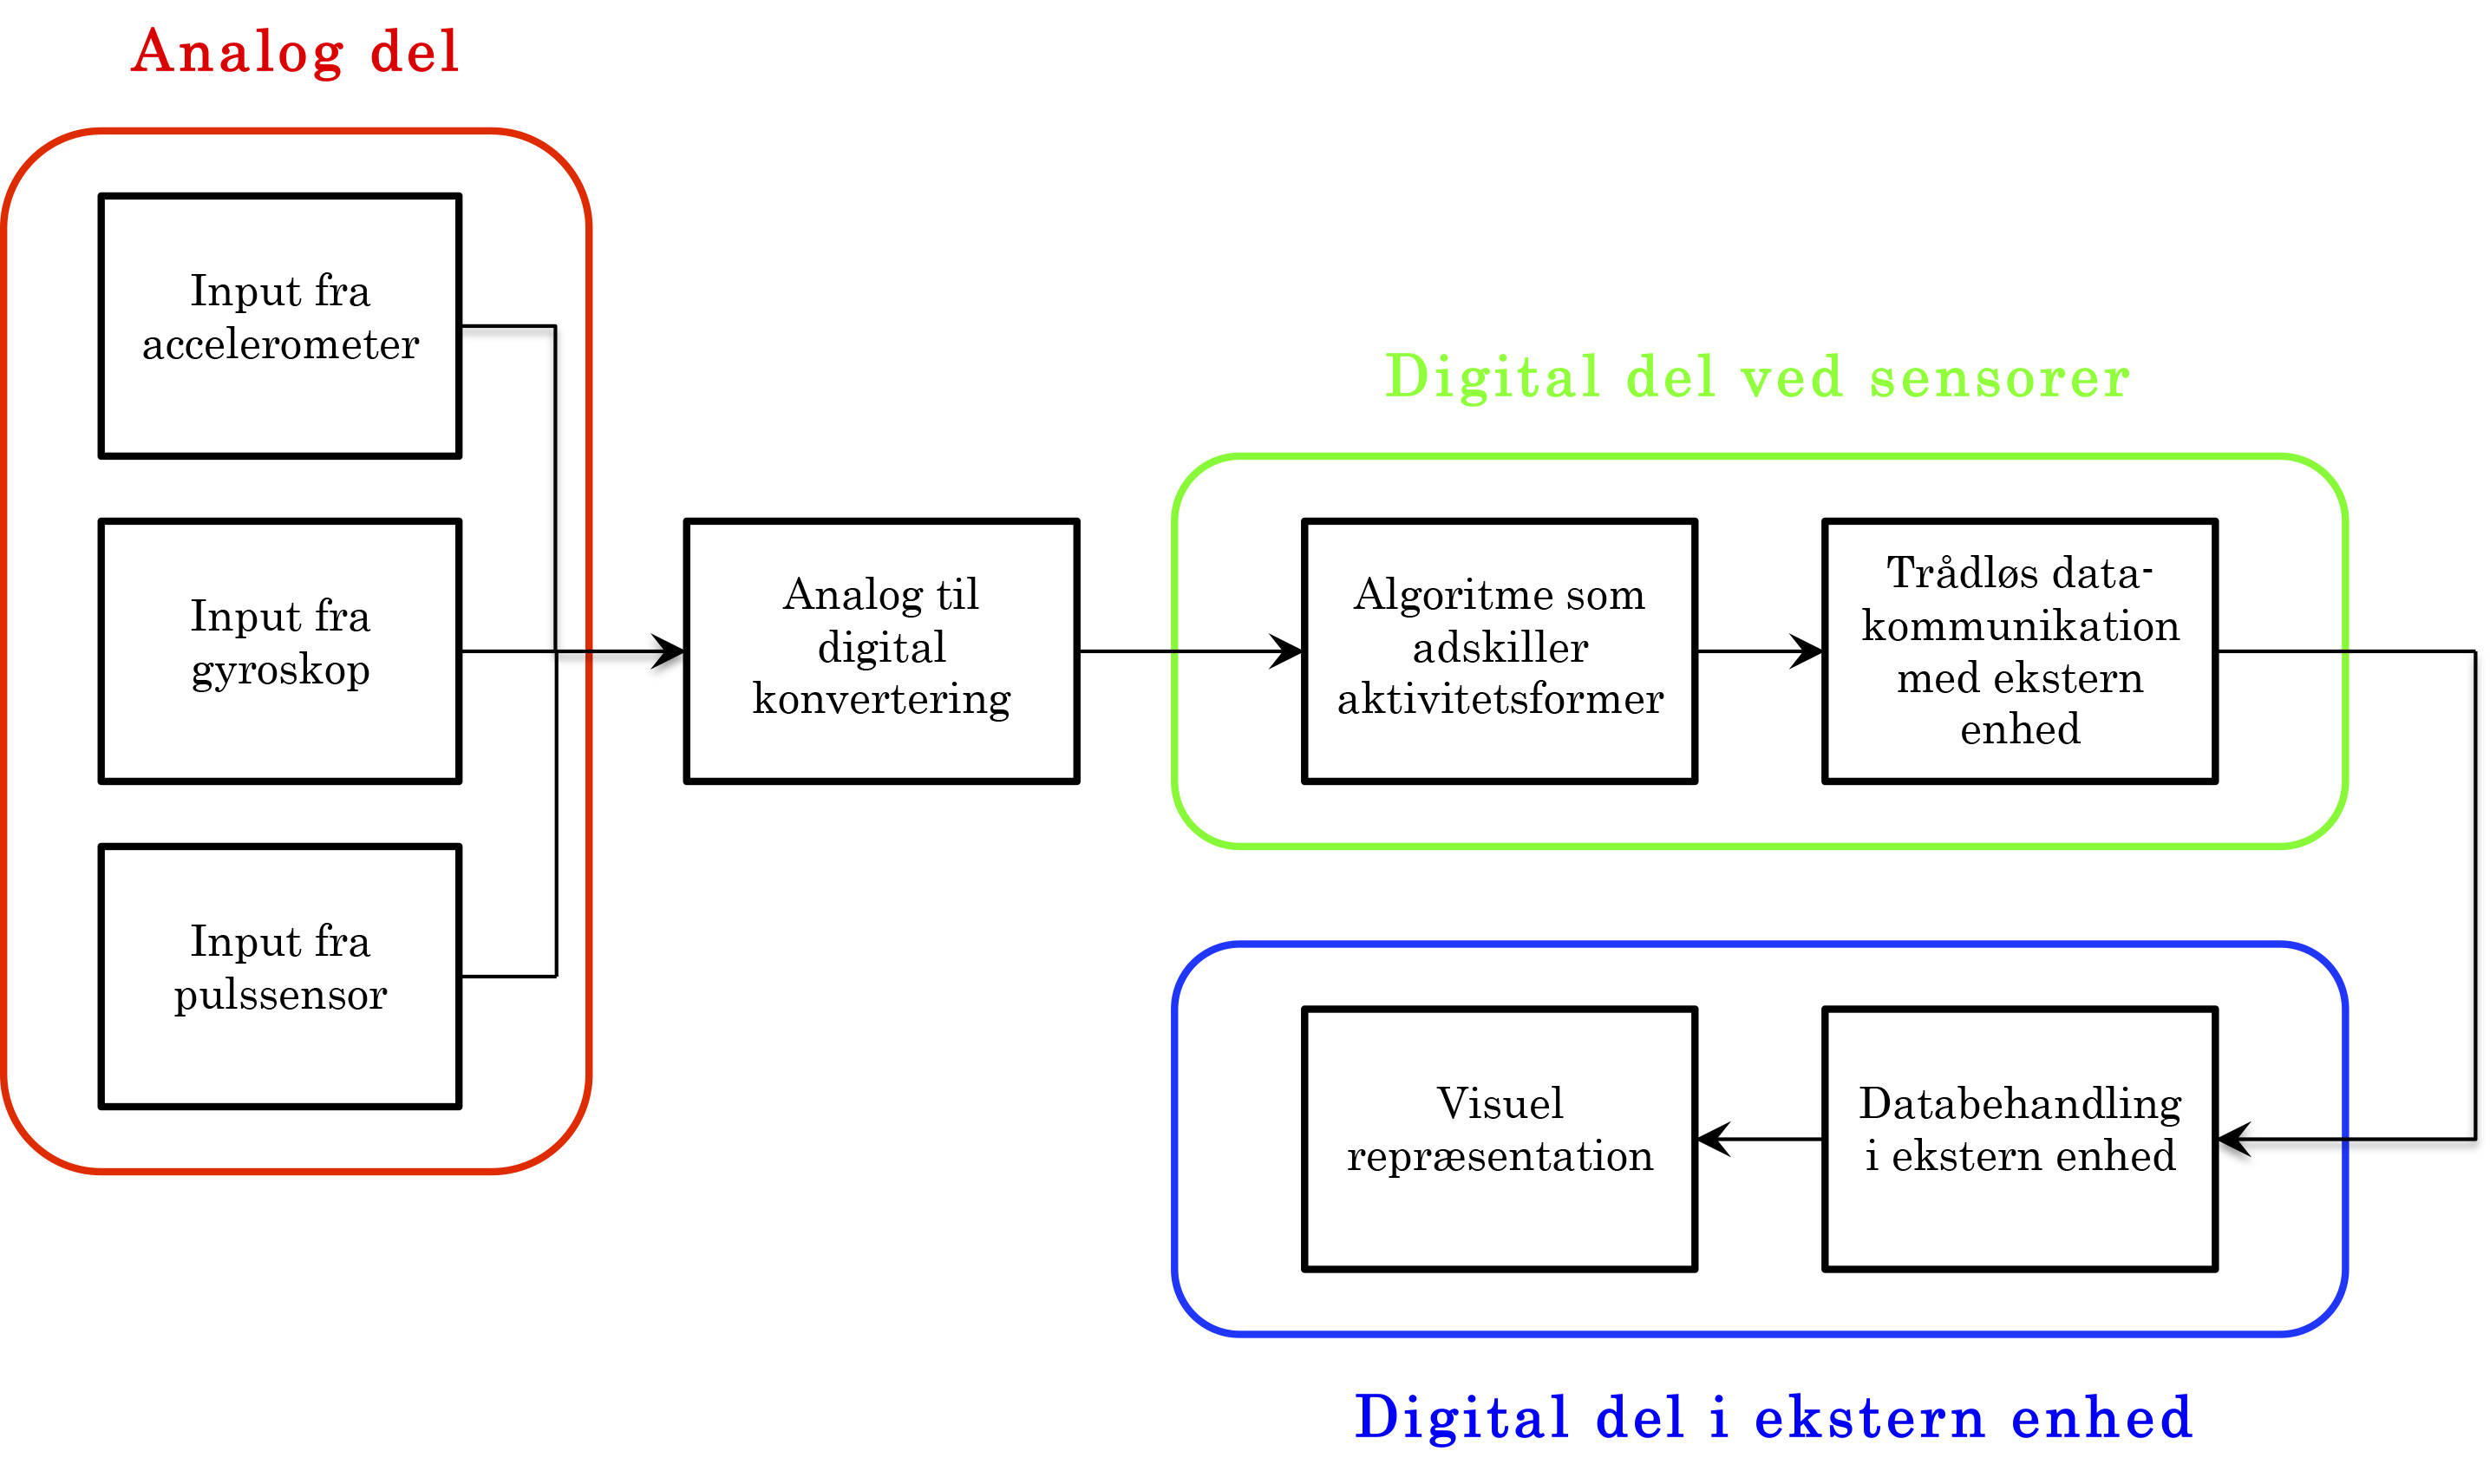
\includegraphics[scale=0.45]{figures/bProblemloesning/blokdiagram.png}
	\caption{På figuren ses blokdiagrammet for det samlede system, hvor et input modtages fra brugeren gennem sensorer, hvilket behandles i en GAP peripheral. Herefter sendes data ved brug af BLE til en computer gennem en GAP central, hvor det visualiseres i en GUI.}
	\label{fig:design_blokdiagram}
\end{figure}\vspace{-0.25cm}
Blokkene implementeres forskellige steder i det samlede system, som vist på \figref{fig:design_blokdiagram}. Spændingsforsyningen tilkobles GAP peripheral, hvor sensorer også tilkobles. På denne MCU vil signalerne blive digitaliseret, og algoritmer vil efterfølgende behandle og adskille aktiviteterne gang, løb og cykling samt udregne en tilhørende puls. Algoritmen og krav hertil står i \secref{krav_algoritme} som én samlet enhed, men i det efterfølgende vil der være to algoritmeafsnit til behandling af data fra henholdsvis accelerometer og gyroskop. Disse data sendes via BLE til en GAP central, som er tilkoblet en computer. På computeren visualiseres dataet i en GUI, hvor brugeren kan følge sin progression.
\section{Spændingsforsyning}\label{spaendingsforsyning}
\textit{Dette afsnit beskriver design, implementering og test af spændingsforsyningen til MCUen, der agerer GAP peripheral.}

\subsection{Design}
MCUen er funktionel ved en spændingstilførsel på 1,71-5,5~V~\citep{Semiconductor20164200M,Semiconductor2016PRoC}. GAP central tilsluttes USB, hvormed den får en spænding på 5~V~\citep{Semiconductor2016}. Derimod skal GAP peripheral tilkobles en ekstern spændingskilde. Spændingsforsyningen skal derfor levere en spænding indenfor det foreskrevne interval. Ydermere vil det blot være MCUens targetboard, som er funktionel ved en ekstern spændingsforsyning.

Den eksterne spændingsforsyning er en batteriholder til to AAA 1,5~V batterier, som har tilkoblet jord og spændingsoutput. Denne komponent er dermed ikke tilkoblet elnettet, hvorfor der er minimal risiko for et farligt elektrisk shock. Yderligere er spændingsforsyningen mobil, hvilket gør den anvendelig i et mobilt system.

\subsection{Implementering}
For at kunne forsyne targetboardet på GAP peripheral skal spændingsforsyningens to ledninger forbindes med pins på MCUen. Spændingsforsyningens to ledninger (GND og Vout) bliver tilkoblet pinrække J1 på targeboardet, hvor pin VDDIO og GND bliver benyttet. De benyttede pins fremgår i \appref{MCU_stor}.

\subsection{Test} 
Testen udføres på baggrund af de opstillede krav og tilhørende afvigelser opstillet i \secref{krav_spaendingsf}. Kravene beskriver, at spændingsforsyningen skal:
\begin{itemize}
	\item Levere mindst 1,71~V og maksimalt 5,5~V til MCUen\fxnote{Alle mikroprocessorer kræver 1,71-5,5~V for at kunne fungere, selvom der står 3,3-5,5~V i databladet for MCUen.}. Der accepteres ikke en spænding uden for grænseværdierne.
	\item Levere minimum 1,71~V i mindst 15~timer. Der accepteres ikke, at spændingsforsyningen leverer under 1,71~V i mindre end 15~timer.
	\item Være mobil og dermed besidde en opsætning som ikke involverer elnettet. Der accepteres ikke en afvigelse i forhold til dette krav.
\end{itemize}
Det undersøges hvilket output spændingsforsyningen har, ved benyttelse af to nye AAA 1,5~V batterier. Testen viser her, at spændingsforsyningen har et output på 3,19~V ved disse betingelser.\newline
Spændingsforsyningen overholder dermed kravet om, at levere en spænding til MCUen i intervallet 1,7-5,5~V. Hvorvidt spændingsforsyningen kan levere den pågældende spænding i dette tidsinterval undersøges i \secref{sec:samlet_system}. Det samlede system skal være funktionelt og komplet før en test kan foretages.
\section{Mikrokontroller}
\textit{I dette afsnit beskrives designet, implementeringen og testen af GAP peripheral som spændingsforsyning til IC og pulssensor.}

\subsection{Design}
GAP peripheral er placeret, således denne MCU er tilkoblet en ekstern spændingsforsyning. Ydermere vil systemets IC og pulssensor være tilkoblet denne MCU, hvorfor disse komponenter vil have MCUen som deres spændingsforsyning. \newline
MCUen har tre pins hvor der er muligt at tilkoble spænding fra en ekstern spændingsforsyning eller tilkoble kombonenters spændingsforsyning. Yderligere har MCUen tre pins hvor ground kan tilkobles. \citep{Semiconductor2016} \newline

Systemets IC indeholder et accelerometer og et gyroskop, hvoraf hele enheden påkræver en spændingsforsyning på 1,9~V til 3,6~V \citep{Jimb02016}.
Ydermere kræver pulssensoren, som også er tilkoblet MCUen, en spændingsforsyning i intervallet 3~V til 5~V \citep{Murphy2016}.

\subsection{Implementering}
Spændingsoutputtet for MCUen er undersøgt, og har påvist et spændingsoutput på 3,14~V ved en tilkobling af en ekstern spændingsforsyning. Dermed overholder spændingsoutputtet fra MCUen, det spændingsinterval som systemets IC påkræver. Spændingsoutputtet overholder desuden intervallet for pulssensorens spændingstilkobling. \newline

Spændingsforsyningen til pulssensoren og ICen vil blive forbundet ved brug af række J2 på targetboardet. VDDA og GND benyttes til at forsyne ICen, men VDDD og GND fra J2 pinrækken benyttes til spændingsforsyning og ground til pulssensoren. \newline
%Ydermere konfigureres det pågældende pins i PSoC Creator, således den pågældende sensor vil blive forbundet med de rigitge pins i forhold til spændingstilkoblingen.


\subsection{Test}

\begin{itemize}
	\item Levere 1,9~V til 3,6~V til ICen. Der accepteres ikke, at pulssensoren modtager en spænding under minimumsgrænsen eller over maksimumsgrænsen.
	\item Levere mellem 3~V og 5~V til pulssensoren. Der accepteres ikke, at pulssensoren modtager en spænding under minimumsgrænsen eller over maksimumsgrænsen.
\end{itemize}

UNDERSØGE HVORVIDT DE GIVNE PINS OVERHOLDER KRAVENE

Mikrokontrollerens outputspændinger skal testes, således output pins i J1 og J2 rækken henholdsvis leverer 3,3 V og mellem 3 - 5 V. Resultatet fra testen beskrives i \tabref{tab:design_mikrokonsp}:
\begin{table}[H]
	\centering
	\begin{tabular}{cccc} \hline
		\rowcolor[HTML]{C0C0C0} 
		Outputpin & Spænding inden pedometer [V] &  Spænding efter pedometer [V] & \begin{tabular}[c]{@{}c@{}}Afvigelse fra\\ønsket værdi [\%] \end{tabular} [\%] \\ \hline
		VDDIO & 4,663 & 3,341 & 1,24 \\ \hline
		VDDD & 4,666 & & 0 \\ \hline
	\end{tabular}%
	\caption{I tabellen ses det, at multimetret nedsætter spændingen, som skal forsyne IC'en. Derudover ses det, at spændingsforsyningen fra MCU'en derved overholder kravene.}
	\label{tab:design_mikrokonsp}
\end{table}\vspace{-0.2cm}
MCU'ens spændingsforsyning til IC'en er hermed justeret ved hjælp af et pedometer, således IC'en i teorien er funktionel. Derudover overholder MCU'ens spænding fra VDDD kravet til pulssensoren. MCU'en er derfor klar til at blive benyttet i det samlede system som spændingsforsyning til IC og pulssensor.
\section{Analog til digital konvertering}
\subsection{Design}
I mikrokontrolleren findes en 12 bits 1 mega sample per sekund (Msps) SAR ADC. Mikrokontrollerens 12 bits ADC kan inddele det analoge signal i $2^{12} = 4096$ spændingsniveauer og skal bruge 18 clocks for at fuldføre en 12 bits konvertering af data med samplingsfrekvens på 18.000.000 Hz, hvilket er dens maksimale samplingsfrekvens. Den understøtter både single ended og differential inputs og kan skanne alle 16 kanaler automatisk. \citep{Semiconductor20164200M,Moore2004}
\section{LSM9DS1}\label{sec_design_LSM9DS1}
\textit{kursiv tekst...}
\subsection{Design}
Der benyttes et integrated circuit (IC) af typen LSM9DS1, der kræver 3,3V for at være optimal funktionel. Denne indeholder magnometer, gyroskop og accelerometer, hvoraf magnometret ikke benyttes. Det er muligt at indstille accelerometeret til $\pm$1, $\pm$4, $\pm$8 eller $\pm$16 g, og gyroskopet kan indstilles til $\pm$245, $\pm$500 eller $\pm$2000 grader per sekund. \citep{Jimb02016,STMicroelectronics2016} Grundet kravene i \secref{Sec:krav} vælges accelerometret til at optage $\pm$16 g og gyroskopet indstilles til $\pm$2000 grader pr sekund. \\
LSM9DS1 har ni frihedsgrader, hvilket betyder, at den måler i x-, y- og z-aksen for både magnometret, gyroskopet og accelerometeret, som kan ses på \figref{vores_IC}. %Akserne for gyroskopet og accelerometeret internt følger højrehåndsreglen.
\citep{STMicroelectronics2016}\newline 
\begin{figure}[H]
	\centering
	\includegraphics[scale=0.6]{figures/cDesign/LSM9DS1.png}
	\caption{På figuren ses akserne fra LSM9DS1. Til venstre ses magnometret, hvis akser er drejet én omgang i forhold til de to andre sensorer. I midten ses gyroskopet med sine roterende akser og til højre ses accelerometerets akser.\citep{Jimb02016}}
	\label{vores_IC}
\end{figure}

Sensoren besidder fire pins på sin venstre side, som vil blive benyttet i dette projekt. Disse kan ses på \figref{fig:IC_pins}. GND og VDD er jord og strømforsyningspins, mens SDA er I$^2$C datapin, hvor al data bliver sendt og modtaget igennem, og SCL er en seriel clock, der blandt andet sørger for synkron datasampling.
\begin{figure}[H]
	\centering
	\includegraphics[scale=0.3]{figures/cDesign/accelerometeret.png}
	\caption{På figuren ses pinkonfigurationen af LSM9DS1. \citep{Jimb02016}}
	\label{fig:IC_pins}
\end{figure}
LSM9DS1 er en digital sensor, hvormed de analoge signaler konverteres til digitale i IC'en ved hjælp af en indbygget 16 bits ADC. Derfor skal sensoren indstilles til en bestemt samplingsfrekvens igennem algoritmedesignet til den. Ifølge \secref{sec:krav} skal accelerometret sample med mindst 450 Hz. Databladet informerer om, at accelerometret kan samples med seks værdier, hvoraf to steps er 238 eller 476 Hz. Derfor vælges samplingen for accelerometret til 476 Hz. Gyroskopet skal samples med mindst 60 Hz, men ifølge gyroskopets datablad kan den enten indstilles til 59,5 eller 119 Hz, hvorfor den indstilles til 119 Hz.

Det digitaliserede signal kan både bruges med en SPI og en I$^{2}$C styrefunktion, hvor mikrokontrolleren CY8CKIT-043 PSoC 4-M besidder begge. Der ønskes at benytte I$^{2}$C funktionen, da ICen dermed både skal sende og modtage data.\fxnote{Modtage om gyroskopet skal tændes eller slukkes.} For at gøre dette skal koden i algoritmedesignet benytte I$^2$C metoden til at skrive til et bestemt registor. På \figref{Fig:master_slave} ses kommunikationen mellem en master og slave, hvoraf slaven i dette tilfælde er ICen og masteren er MCUen.\fxnote{Og dette kan ikke vendes om, ICen vil ALTID være slaven} Der ses, at MCUen skriver en start kode til ICen for at starte kommunikationen. Herefter skriver masteren én bit til slaven, som skal godkende, at dette er modtaget. Så vil masteren give en adresse til slaven, som bestemmer hvorfra sensoren skal give data. Når slaven har godkendt dette, skriver masteren til slaven, at den gerne vil læse fra slaven, hvilket tillades og data hentes over på masteren. Afslutningsvist skriver masteren en stop kode til slaven, hvorefter kommunikationen er afbrudt. %For at benytte I$^{2}$C funktionen sættes pin CS\_AG høj, og de fire pins SDO og CS benyttes ikke. Alle pins kan ses på \figref{IC_pins}. Før et signal kan registreres kobles pinnen GND til jord, og på benet VDD skal der leveres mellem 1,9 V og 3,6 V.\fxnote{skriv resten af opsætningen efter at have snakket med John}. 
\begin{figure}[H]
	\centering
	\includegraphics[scale=0.75]{figures/cDesign/Sensor_write_read2.png}
	\caption{På figuren ses metoden for kommunikation imellem slave og master enhed. Denne kan udvides og gøres mere kompleks i tilfælde at, om masteren vil henholdsvis læse eller skrive en eller flere bits.\citep{STMicroelectronics2016}}
	\label{Fig:master_slave}
\end{figure}
I LSM9DS1 forbruger gyroskopet 4 mA og accelerometeret 600 $\mu$A ved normale betingelser\fxnote{hvor Vdd er forsynet med 2,2V og temperaturen er 25 grader}. Det er derfor essentielt, at gyroskopet bruges så lidt som muligt, når systemet skal være batteridrevet og kun benytter accelerometret til datasampling. Det er muligt enten at slukke begge sensorer, at benytte accelerometeret alene eller benytte både accelerometeret og gyroskopet sammen, hvor begge har samme mængde output af data. Der kan yderligere spares strøm ved brug af gyroskopet, hvis der vælges en lavere samplerate.\\ % alt efter hvor hurtigt et signal skal samples. 
Gyroskopet har tre forskellige power modes: slukket, low power og normal power. For at gyroskopet kan være i low power, skal outputtet af data være på 14,9-119 Hz. Hvis outputsignalet er over dette, vil gyroskopet automatisk gå i normal power. Ifølge \secref{Sec:krav} skal gyroskopet samples med mindst 60 Hz, men samplingen kan enten være 59,5 eller 119, hvorfor den indstilles til 119 Hz. Derfor kan gyroskopet til dette projekt køre i low power mode. \citep{STMicroelectronics2016}
%Accelerometeret og gyroskopet har 32 åbninger af 16 bit data FIFO til hver af gyroskopets akser, samt 16 bit FIFO til hver af accelerometerets akser. Derved skal data ikke konstant sendes til en enhed og der kan spares strøm. Bufferen kan virke på fem forskellige måder, hvor der er tre overordnede tilstande: Bypass tilstand, FIFO tilstand og kontinuert tilstand, som alle tre er illustreret på \figref{tilstand}. Derudover er der to kombinerede tilstande: kontinuert-til-FIFO tilstand og bypass-til-kontinuert tilstand. \newline
%\begin{figure}[H]
%	\centering
%	\includegraphics[scale=0.28]{figures/cDesign/LSM9DS1_tilstand.png}
%	\caption{På figuren ses de tre overordnede tilstande IC'en kan opsamle data med.\citep{Jimb02016}}
%	\label{tilstand}
%\end{figure}
%I bypass tilstanden bruges kun den første adresse, som overskrives når ny data er tilgængelig. Denne tilstand benyttes blandt andet til at nulstille FIFO
%FIFO stilstanden bruges til at lagre data i niveauer indtil ny data overskriver det gamle. Det er muligt at gemme data i 32 niveauer, men dette kan tilpasses mindre efter behov. For at gammel data ikke overskrides indsættes et interrupt når FIFO er fyldt, hvormed der ikke lagres ny data. 
%Den kontinuerte tilstand muliggør kontinuert FIFO, hvormed ny data overskriver gammel data. 
%Ved kontinuert-til-FIFO tilstand skifter tilstanden alt efter de bit der modtages i interruptet for accelerometeret og gyroskopet. Hvis der modtages et bit på 1 vil den være i FIFO tilstand, og modtages der et bit på 0, vil den være i kontinuert tilstand. 
%I bypass-til-kontinuert tilstand skiftes der ligeledes mellem bypass og kontinuert tilstand alt efter det modtagne interrups for accelerometeret og gyroskopet. Hvis der modtages et bit på 1, er den i kontinuert tilstand, og modtages der en bit på 0, nulstilles den ved at gå i bypass tilstand. 
\subsection{Implementering}
For at kunne implementere sensoren således at MCUen kan modtage data fra den, skal MCUen besidde en algoritme, der får sensoren til at sende data. MCUen skal skrive til hex adressen 6B, som er registeradressen for gyroskopet og accelerometer. Således kan MCUen som master skrive til selve accelerometret eller gyroskopet. Via hexkoderne A8 og 79 indstilles accelerometret og gyroskopet til de valgte indstillinger, som er sampling på 476 Hz og 16 g måling for accelerometret og sampling på 119 Hz og 2000 grader pr sekunds målinger for gyroskopet. De binære koder for korrekt indstilling af sensorerne kan findes i databladet. \citep{STMicroelectronics2016}\\
I PSoC Programmer indhentes det analoge komponent I2CM. Denne skaber en I$^2$C forbindelse imellem MCUen og ICen samtidig med, at den indstiller MCUen til at være master. Når PSoC Programmer benyttes til test af sensoren er der ikke behov for flere komponenter, men hvis dataen skal sendes ind i eksempelvis matlab, kræver det en UART. I2CM modulet skal indstilles til korrekte pins i topdesignet af algoritmen, således sensorens SDA og SCL pins kobles korrekt til MCUen.
% SKRIV NOGET OM GROUND OG VDD FORBINDELSEN, FOR PT FÅR DET JO IKKE STRØM FRA MCUEN
\subsection{Test}
Accelerometret er indstillet til $\pm$16 g igennem algoritmedesignet, hvorfor det antages, at den kan opsamle op til $\pm$16 g. Ifølge accelerometrets andet krav i \secref{sec:krav} skal det angive korrekt g påvirkning med en maks afvigelse på 5\%. Dette testes ved at påvirke sensorens y akse med $\pm$1 g, da denne akse på accelerometret benyttes til detektering af gang og løb, se \secref{bevaegelse}. Gyroskopet antages at måle korrekt, da projektgruppen ikke er i besiddelse af korrekt måleudstyr, der har konstant acceleration.\\
ICens accelerometer har en sensitivitet på 0,732 mg per LSB \citep{STMicroelectronics2016}. Outputtet fra sensoren igennem MCUen er LSB, da den optager low og high byte for hver akse. Igennem bitskift af high byte og addition af de to bytes giver sensoren LSB i output. 

Inden test tjekkes bordet med vaterpas for at sikre, at accelerometrets y akse ikke påvirkes af den grund. Herefter placeres accelerometret vandret på bordet. Når accelerometret vendes i $\pm$90$^\circ$ på y aksen, påvirkes denne af henholdsvis $\pm$1 g. I \tabref{tab:test_sensor} ses resultatet fra testen.
\begin{table}[H]
	\centering
	\begin{tabular}{cccc} \hline
		\rowcolor[HTML]{C0C0C0} 
		Teoretisk & \begin{tabular}[c]{@{}c@{}} Output fra MCU \\ (LSB) \end{tabular} & \begin{tabular}[c]{@{}c@{}} Omregnet \\ (g) \end{tabular} & \begin{tabular}[c]{@{}c@{}} Procent afvigelse \\ (\%) \end{tabular} \\ \hline
		0 g påvirkning & 19 & 19$\times$0,000732 = 0,014 g & 1,4\\ \hline
		-1 g påvirkning & 1368 & 1368$\times$0,000732 = 1,003 g & 0,3\\ \hline
		+1 g påvirkning & -1356 & -1356$\times$0,000732 = 0,993 g & 0,7\\ \hline
	\end{tabular}%
	\caption{I tabellen ses resultatet fra testen af accelerometrets y akse.}
	\label{tab:test_sensor}
\end{table}\vspace{-0.2cm}
Det ses i \tabref{tab:test_sensor}, at accelerometret overholder kravene fra \secref{sec:krav}. Denne enhed accepteres derfor og er klar til videre implementering.
%Accelerometrets sensitivitet ved 16 g målinger: 0,732 mg/LSB
%Hvor LSB er 2*16/2^16 = 0.0078125
%(Man får et output på ca. 1350 fra acc, hvilket giver næsten 1 ganget med 0,732 mg/LSB)
%
%Gyroskopets sensitivitet med 2000 dps målinger: 70 mdps/LSB
%Hvor LSB er 2*2000/2^16 = 0.97656
%()
\section{Pulssensor}\label{sec_design_puls}
\textit{I dette afsnit beskrives designet, implementeringen og testen af den valgte pulssensor.}

\subsection{Design}
Pulssensoren SEN-11574 er valgt til dette projekt, da det er en optisk pulssensor og er derfor mere sikker for brugeren, som beskrevet i \secref{sec:pulssensor}. Derudover er en optisk pulssensor mere alsidig i forhold til placering, da den blot skal placeres over en arterie. En elektrisk pulssensor har risiko for at opfange muskelkontraktion frem for puls, hvis den ikke placeres korrekt. Pulssensoren SEN-11574 kræver 3 til 5 V for at være funktionel og forbruger 4 mA ved en forsyning på 5V. På sensorens board findes et aktivt filter\fxnote{Et aktivt filter er en type af analog elektronisk filter, der anvender aktive bestanddele, såsom en forstærker.} samt en forstærker, som tilsammen øger amplituden for pulsbølgen og normaliserer signalet omkring et referencepunkt, hvilket fjerne al DC spænding i signalet. Herved fremkommer en tydelig pulsbølge direkte fra sensoren, som umiddelbart ikke kræver behandling af signalet for at kunne detektere. \citep{Murphy2016,Murphy2016_sensor}

\subsection{Implementering}
Pulssensoren skal benyttes til at beskrive intensiteten af aktiviteten, som beskrevet i \secref{subsub:ak_int}. Herudfra kan effekten af aktiviteten bestemmes, hvilket kan have en motiverende faktor for brugeren. \\
Sensoren har 3 pins til henholdsvis spændingsforsyning, ground og outputsignal, som skal kobles med MCU'en. Outputsignalets pin skal designes i programmet PSoC Creater, således MCU'en kan finde ud af at modtage signalet fra denne pin. Dette gøres ved at indsætte henholdsvis en UART serie kommunikationsblok (SCB) og SAR ADC i topdesignet. UART'en bruges for at sensoren og MCU'en kan kommunikere og er tilpasset formålet fra standart. Puls data skal igennem en ADC, da det er et analog signal, der fortsætter så længe sensoren modtager en spænding. Dennes design skal derfor tilpasses pulssensoren, hvilket gøres ved at vælge antallet af kanaler og indstille sampleraten. I dette tilfælde skal der benyttes én kanal, som er single ended, og ADC'ens samplingsfrekvens sættes til 35 SPS. ADC'ens samplingsfrekvens vælges ud fra, at en persons makspuls kan beregnes med 220 - alder \citep{CooperBlair2005}. Ud fra målgruppen vurderes det, at makspulsen altså er cirka 210, som svarer til tre et halvt slag pr sekund. Det vurderes at ti samples per puls giver et præsentabelt resultat, hvilket derved giver 35 SPS.\\
Efter UART og ADC er konfigureret i topdesignet, skal de korrekte pins indstilles i pinopsætning. UART pins får typisk tildelte interne pins, hvorimod ADC'ens inputpin skal indstilles til den plads, som outputtet fra sensoren er. I dette tilfælde er det pin 2.0. Når overstående design er implementeret, indstilles MCU'en til at debugge via programmet PSoC Creater. \\

Igennem et matlab program er det muligt at visualisere pulsen ved hjælp af en GUI. I det samlede system skal denne GUI ikke være tilgængelig her i processen, da GAB peripheral modtager pulsdata og sender dette videre sammen med IC data til GAB central, som skal visualisere data i en endelig GUI.\\
I matlabscriptet vælges den pågældende port for MCU'en i computeren, således PC'en kan registrere hvor det visualiserede data skal komme fra. Herefter startes scriptet og en figur tvinges i front med pulsen, hvor et bestemt antal sekunders vindue visualiseres

\subsection{Test}
Pulssensoren skal testes for, om den kan opfange brugerens puls under fysisk aktivitet uden ukorrekt eller ikke tydelig puls. Dette gøres ved, at der optages to målinger henholdsvis med og uden fysisk aktivitet, hvor sensoren placeres på den distale phalanges på højre hånds pegefinger. Ud fra matlab scriptet og tilhørende optagede data vurderes det, om pulsen visualiseres korrekt, således den korrekte puls kan kalkuleres.\\
Den fysiske aktivitet bestod af gang på et løbebånd. Hver måling optages i 10 sekunder, hvilket ses på \figref{fig:puls_m_u}.\\
%\begin{figure}[H]
%	\centering
%	\includegraphics[scale=0.6]{figures/cDesign/ToPulser.png}
%	\caption{På figuren ses to plots for hver test af pulssensoren. På figur 1 til venstre står forsøgspersonen helt stille i 10 sekunder, hvorimod vedkommende går i en subjektiv vurdering af normal gang på figur 2 til højre. Der ses en tydelig puls på figur 1, hvorimod pulsen ikke fremgår på figur 2.}
%	\label{fig:puls_m_u}
%\end{figure}
Matlab scriptet udregnede

% Test af krav


% Grimme hjemmeside \citep{Murphy2016}
% \cite{Murphy2016_sensor}
\section{Algoritme til detektering af gang og løb}\label{sec:algogangloeb}
\textit{Dette afsnit omhandler design, implementering og test af algoritmerne til detektering af aktiviteterne gang og løb. Først designes algoritmen til detektion af henholdsvis gang og løb, hvorefter denne implementeres. Afslutningsvist bliver algoritmen testet i forhold til de opstillede krav i \secref{krav_algoritme}.} 
%bliver design af algoritmerne behandlet, hvilket er ensbetydende med at implementering og kodning kan foregå. Når algoritmerne er designet og implementeret bliver de efterfølgende testet for at af- eller bekræfte deres virkning.}

For at kunne adskille gang og løb benyttes et accelerometer, som er beskrevet i \secref{sec_design_LSM9DS1}. For at kunne detektere og adskille disse aktiviteter behandles inputtet fra sensoren gennem forskellig signalbehandlingsprocessor. Algoritmerne gør det muligt at afgøre, om de pågældende signaler repræsenterer gang, løb eller ingen fysisk aktivitet. 

\subsubsection{Design} \label{design_algo_g_l}
Algoritmen som skal detektere gang eller løb designes til at benytte accelerometerets data, med henhold til \appref{pilot}. Dette design fremgår som flowchart på \figref{fig:design_algoritme_gang_loeb}.
\begin{figure}[H]
	\centering
	\includegraphics[scale=0.5]{figures/cDesign/design_algoritme_gang_loeb.png}
	\caption{På figuren ses et flowchart over algoritmen til detektering af ingen fysisk aktivitet, gang og løb.}
	\label{fig:design_algoritme_gang_loeb}
\end{figure}
Algoritmen skal benyttes accelerometerets data til at detektere hvorvidt brugeren ikke udfører fysisk aktivitet, går eller løber. \\
Førend denne detektering, skal accelerometeres data signalbehandles for afslutningsvis at kunne benytte tærkselværdier til at detektere hvilken aktivitet der udføres. Signalbehandlingen indebærer filtrering, dividering, kvadrering og moving average filtrering. Denne type signalbehandling af illustreret på \figref{fig:algoritme_behandling}.
\begin{figure}[H]
	\centering
	\includegraphics[width=1\textwidth]{figures/cDesign/signalbehandling_psoc.png}
	\caption{På figuren ses de fire signalbehandlingsfunktioners effekt på rå data fra accelerometeret under løb. Den sorte kurve på de fire figurer er det rå signal, og den røde er det behandlede output. Der gøres opmærksom på, at y-aksen ikke er ens for henholdsvis de to øvre og de to nedre figurer, hvorfor det sorte, rå signal bliver en næsten lige linje på de to nedre figurer.}
	\label{fig:algoritme_behandling}
\end{figure}
Signalbehandlingen har til formål at tydeliggøre hælnedslag, for derefter at kunne implementere tærskelværdier til adskillelse af de fysisk aktiviteter. \\
Første del af signalbehandlingen er en filtrering med et elliptisk båndpassfilter, som benyttes til at dæmpe støj. Dette skal være et fjerde ordens elliptisk båndpasfilter med et pasbånd fra 20~Hz til 50~Hz, og med en dæmpning på 60~dB\fxnote{og 0.5 dB peak-to-peak ripples - frekvenserne for gang og løb lå mellem 25 og 45}. Båndpasfilterets knækfrekvenser er valgt med hensyn til pilotforsøget i \appref{pilot}, hvorfra det vurderes at hælnedslag har en frekvens på 25~Hz til 45-~Hz. Ved at benytte et båndpass filter bliver det ønskede signal i frekvensområdet 25-45~Hz bevaret, og andre frekvensen dæmpes.\\
Dernæst bliver signalet behandlet ved brug af en division, som har til formål at sænke amplituden af mindre spikes i signalet. Idet hælnedslaget har den største amplitude i signalet, da bliver amplituden for hælnedslaet fortsat større end de mindre spikes, efter divisionen har indtruffet. \\
Efter signalet er blevet divideret, da kvadreres dette for dermed at øge amplituden af de fremtrædende spikes i signalet. Dermed minimeres de mindre spikes kraftigt, som ikke relateres til hælnedslaget, og selve hælnedslaget forstærkes og tydeliggøres. \\
Afslutningsvis filtreres signalet med et moving average filter, som udglatter signalet, hvorved små udslag ikke opfattes, og signalets hælnedslag vil fremstå som et enkelt spike.

Ovenstående signalbehandling giver et signal med peaks, som skal adskilles med tærskelværdier for henholdsvis gang og løb. Førend en værdi for denne tærskelværdi kan fastsættes, skal dataet fra pilotforsøgets omregnes til ICens enhed for outputdata. ICens arbejdsområde er opgivet i bytes, som følge af ICens 16 bits ADC arbejdsområde. Pilotforsøgets data skal derfor omregnes til bytes, idet data fra pilotforsøget er optaget med Shimmer3 som har enheden, $m/s^{2}$. Derfor bliver pilotforsøgets data først omregnet til g, hvorefter denne være omregnes med henhold til opløsningen for den 12 bits ADC som er placeret i Shimmer3. For at gøre dette benyttes accelerometerets sensitivitet, som er 0,012 g/LSB. Data fra shimmer som er omregnet til g, skal divideres med accelerometerets sensitivitet. Outputet fra Shimmer3 og ICen er nu samme enhed, som det fremgår af \eqref{eq:bitsammenhaeng}.
 
\begin{equation}
\frac{32 g \cdot 2^{16}}{32 g \cdot 2^{12}} = 16
\label{eq:bitsammenhaeng}
\end{equation}

Data fra Shimmer3 skal derfor multipliceres med 16, hvilket medfører samme enhed for de to systemer. Det er derefter muligt, at vurdere hvilket tærskelværdier som kan benyttes til at detektere gang og løb.\\
De behandlede signaler fra pilotforsøget, benyttes med henblik på fastsættelse af tærskelværdier. \tabref{tab:individuel_taerskel} viser tærskelværdierne for de fire forsøgspersoner, hvoraf tærskelværdierne er bestemt med henhold til de behandlede signaler. 
\begin{table}[H]
	\centering
	\begin{tabular}{ccc}
		\hline
		\rowcolor[HTML]{C0C0C0} 
		Forsøgsperson & Tærskelværdi for gang & Tærskelværdi for løb \\ \hline
		\rowcolor[HTML]{FFFFFF} 
		F1 & 50 & 1050 \\ \hline
		\rowcolor[HTML]{FFFFFF} 
		F2 & 55 & 500 \\ \hline
		\rowcolor[HTML]{FFFFFF} 
		F3 & 50 & 400 \\ \hline
		\rowcolor[HTML]{FFFFFF} 
		F4 & 150 & 100 \\ \hline
	\end{tabular}
	\caption{I tabellen ses tærskelværdierne for forsøgspersonerne ved aktiviteterne gang og løb.}
	\label{tab:individuel_taerskel}
\end{table}\vspace{-0.5cm}
De individuelle tærskelværdier i \tabref{tab:individuel_taerskel} er fundet over et fem sekunders vindue for hver forsøgsperson. Heraf antages det, at tærskelværdierne er repræsentative for den fysiske aktivitet idet aktiviteten blev udført ved konstant hastighed. Ydermere skal systemet være gældende for en stor population, hvormed en given tærskelværdierne for gang og løb skal være dækkende for alle forsøgspersoner. En samlet tærskelværdi, der er dækkende for samtlige forsøgspersoners data, ses i \tabref{tab:faelles_taerskel}.
\begin{table}[H]
	\centering
	\begin{tabular}{ccc}
		\hline
		\rowcolor[HTML]{C0C0C0} 
		Tærskelværdi for ingen fysisk aktivitet & Tærskelværdi for gang & Tærskelværdi for løb \\ \hline
		x \textless~50 & 50 \textless~x~\textless 400 & x~$\geq$~400 \\ \hline
	\end{tabular}
	\caption{I tabellen ses de tærskelværdier, som for alle forsøgspersoner vil kunne detektere og adskille gang og løb fra hinanden.}
	\label{tab:faelles_taerskel}
\end{table}\vspace{-0.5cm}
Fastsættelsen af den fælles tærskelværdi bør sikre, at gang og løb er mulige at detektere samt adskille for forsøgspersonernes data. Igennem behandling af data fra pilotforsøget forekom tærskelværdierne i \tabref{tab:faelles_taerskel} dækkende for alle forsøgspersonerne, hvorfor disse blev valgt.

\subsection{Implementering}
Implementeringen af algoritmen for detektering af gang og løb tager udgangspunkt i data fra pilotforsøget og de designmæssige aspekter, som er beskrevet i \secref{design_algo_g_l}. Algoritmen er designet og implementeret, som det ses på \figref{fig:basic_algo_g_l}.
\begin{figure}[H]
	\centering
	\includegraphics[scale=0.6]{figures/cDesign/Algoritme_g_l_basic.png}
	\caption{På figuren ses den overordnede C kode for algoritmen til detektering af gang og løb beskrevet med pesudokode. De markerede kasser vil blive forklaret yderligere i kommende figurer.}
	\label{fig:basic_algo_g_l}
\end{figure} \vspace{-0.5cm}
Algoritmen henter low og high byte fra ICens outputdata, hvorefter de enkelte samples gennemgår en signalbehandling. Denne signalbehandling og den tilhørende C kode vil blive yderligere forklaret i \figref{fig:signalbehandling_g_l}. Efter samples er blevet behandlet, bliver time\_counteren startet således, at denne tæller antallet af samples mellem bestemte if lykker i algoritmen. De behandlede samples gemmes i variabel Value[0], hvortil den foregående behandlede sample bliver gemt i variabel Value[1]. På denne måde, hvorpå en gammel og ny sample gemmes i hver sin variabel, muliggøres blandt andet, at algoritmen kan undersøge disse variabler i forhold til hinanden og deres størrelse i forhold til en tærskelværdi. \\
Efter den nye og foregående sample er placeret i separate variabler er det muligt at benytte tærskelværdier til at detektere, hvorvidt der er ingen aktivitet, gang eller løb. Disse elementer af algoritmen forklares yderligere i \figref{fig:ingen_ak_pseudo}, \figref{fig:gang_pseudo} og \figref{fig:loeb_pseudo}. Tærskelværdierne for de pågældende fysiske aktiviteter er bestemt i \secref{design_algo_g_l}. \\ 
Yderligere bliver den maksimale peak bestemt, da denne værdi initialiserer, om det er gang eller løb i GUIen. Dette gøres ved at sammenligne, om den forrige sample er større end den nuværende. Hvis dette er tilfældet, betegnes den forrige værende som værende maks peak værdien. %Når kurven derimod er faldende, vil detektering af maksimale peak ikke udføres.

Algoritmens signalbehandling involverer fire elementer; elliptisk filtrering, dividering, kvadrering og en moving average filtrering. Dette ses på \figref{fig:signalbehandling_g_l}.
\begin{figure}[H]
	\centering
	\includegraphics[scale=0.6]{figures/cDesign/Signalbehandling_gl_pesudo.png}
	\caption{På figuren ses algoritmens signalbehandling i C kode beskrevet som pseudokode.}
	\label{fig:signalbehandling_g_l}
\end{figure} \vspace{-0.5cm}
Efter datamodtagelse fra ICen bliver samples IIR filtreret ved hjælp af a og b koefficienter for et elliptisk filter. Efterfølgende retureneres de behandlede samples, hvormed disse er klar til næste del af signalbehandlingen. De pågældende a og b koefficienter bestemmes i MATLAB, hvor filterets knækfrekvenser og dæmpning benyttes til at bestemme det elliptiske filters koefficienter. Disse koefficienter skriver i C koden for algoritmen, således filtreringen er med henhold til det ønskede filter designet i MATLAB.\\
De enkelte samples bliver herefter bitskiftet med 5, hvilket svarer til at dividere med 32\fxnote{2 opløftet i 5}. Derudover bliver samples kvadreret ved at gange hver sample med sig selv. Afslutningsvis filtreres samples med et moving average filter, hvilket medfører en blødere kurve, som ses på \figref{fig:algoritme_behandling}.

Algoritmen er designet og implementeret således, at denne kan detektere, hvis brugeren ikke er fysisk aktiv. Denne del af algoritmen fremgår af \figref{fig:ingen_ak_pseudo}.
\begin{figure}[H]
	\centering
	\includegraphics[scale=0.6]{figures/cDesign/ingen_aktivitet_gl_pseudo.png}
	\caption{På figuren ses algoritmens metode til at detektere, om brugeren er fysisk aktiv eller ej. Det fremgår, at hvis time\_count er større end tre sekunder sampling, som svarer til 1428 samples, da detekteres brugeren som værende ikke fysisk aktiv.}
	\label{fig:ingen_ak_pseudo}
\end{figure} \vspace{-0.5cm}
Algoritmen detekterer, at brugeren ikke er fysisk aktiv, hvis time counteren opnår et antal samples, som er større end tre sekunders sampling. Hvis dette er tilfældet, bliver de pågældende variabler nulstillet og tæller forfra.

Algoritmen benytter tærskelværdier til at bestemme hvorvidt brugeren går eller løber. \Figref{fig:gang_pseudo} viser algoritmens opbygning med henhold til detektering af gang ved brug af tærskelværdier.
\begin{figure}[H]
	\centering
	\includegraphics[scale=0.6]{figures/cDesign/gang_ckode_pseudo.png}
	\caption{På figuren ses den implementerede C kode beskrevet med pseudokode. Denne del af algoritmen benyttes til detektering af gang.}
	\label{fig:gang_pseudo}
\end{figure} \vspace{-0.5cm}
Til venstre på figuren ses delen, som er ansvarlig for optælling af skridt, hvortil den højre del visualiserer delen, som bestemmer varigheden mellem hælnedslag ved gang. Førend algoritmen kan tælle op på antal skridt for gang, skal amplituden for Value[0] være i intervallet mellem tærskelværdierne for gang og løb. Yderligere skal den foregående sample Value[1] have en værdi, der er lavere end tærskelværdien for gang. Hvis disse tre kriterier er opfyldt, indstilles Trace\_Max til at være lig 1. Dette tillader, at algoritmen begynder at finde den maksimale peak, som illustreret på \figref{fig:basic_algo_g_l}. Ydermere bliver Step\_count\_gang talt op, indtil denne variabel er maksimalt 3. \\
Højre del af \figref{fig:gang_pseudo} repræsenterer den del af algoritmen, som finder varigheden mellem hælnedslag og sender dette gennem BLE. Førend denne del af algoritmen bliver udført, skal Value[0] være mindre end tærskelværdien for gang og Value[1] skal være over denne tærkselværdi. Yderligere skal det bestemte maksimale peak være mindre end tærskelværdien for løb. Hvis kriterierne opfyldes, bliver det maksimale peak gemt i PEAK, samt algoritmen indstilles således, at denne ikke længere finder et maksimalt peak. Yderligere er det gældende, at hvis der er detekteret ét hælnedslag for gang, bliver henholdsvis time counteren og PEAK nulstillet. \\
For at bestemme varigheden mellem hælnedslag skal antallet af hælnedslag for gang overstige værdien 1. Under disse omstændigheder bliver time\_count og PEAK bitskiftet, hvorefter disse værdier sendes over BLE. Afslutningsvis nulstilles time counteren.

Algoritmen er desuden i stand til at detektere løb, hvilket også gøres ved brug af tærskelværdier, som det ses på \figref{fig:loeb_pseudo}.
\begin{figure}[H]
	\centering
	\includegraphics[scale=0.6]{figures/cDesign/loeb_ckode_pseudo.png}
	\caption{ På figuren ses den implementerede C kode beskrevet med pseudokode. Denne del af algoritmen benyttes til detektering af løb.}
	\label{fig:loeb_pseudo}
\end{figure} \vspace{-0.5cm}
Den venstre del af figuren er ansvarlig for optælling af skridt, hvortil den højre del bestemmer varigheden mellem hælnedslag ved løb. Førend algoritmen kan tælle op på antal skridt for løb, skal amplituden for Value[0] være større end tærskelværdien for løb. Yderligere skal den foregående sample Value[1] have en størrelse, der er lavere end tærskelværdien for løb. Hvis disse to kriterier er opfyldt, indstilles Trace\_Max til at være lig 1. Dette tillader, at algoritmen begynder at finde den maksimale peak, som illustreret på \figref{fig:basic_algo_g_l}. Ydermere bliver Step\_count\_løb talt op, indtil denne variabel er maksimalt 3. \\
Højre del af \figref{fig:loeb_pseudo} repræsenterer den del af algoritmen, som finder varigheden mellem hælnedslag og sender dette gennem BLE. Førend denne del af algoritmen bliver udført, skal Value[0] være mindre end tærskelværdien for løb, og Value[1] skal være over denne tærskelværdi. Hvis kriteriet opfyldes, bliver det maksimale peak gemt i PEAK, samt algoritmen indstilles således, at denne ikke længere finder et maksimalt peak. Yderligere er det gældende, at hvis der er detekteret ét hælnedslag for løb bliver henholdsvis time counteren og PEAK nulstillet. \\
For at bestemme varigheden mellem hælnedslag  skal antal hælnedslag for løb overstige værdien 1. Under disse omstændigheder bliver time\_count og PEAK bitskiftet, hvorefter disse værdier sendes over BLE. Afslutningsvis nulstilles time counteren.

\subsection{Test}
Testen udføres med henhold til de opstillede krav og tilhørende tilladte afvigelser opstillet i \secref{krav_algoritme}. Kravene beskriver, at algoritmen skal:
\begin{itemize}
	\item Behandle data fra accelerometret, således hælnedslag fremstår som et markant peak.
	\item Være i stand til at detektere gang og løb ved brug af tærskelværdier. Det accepteres ingen afvigelse ved detektering af den pågældende aktivitet.
\end{itemize}
Algoritmens funktioner testes individuelt og samlet. Dette gøres ved at indsende et simuleret signal, hvis funktion er at agerer som gang, løb eller ingen aktivitet. Det simulerede signal er et absolut sinussignal med varierende amplitude. Amplituden for det simulerede signal afgør, hvorvidt signalet bør agerer som gang, løb eller ingen aktivitet. Et sinussignal er valgt, da dette har grundlæggende samme karateristik som et eventuelt gang- eller løbesignal. Der ønskes et ideelt signal, som går over og under tærskelværdierne og derved kan aktivere timeren i algoritmen.

Først testes algoritmens time counter, der giver et udtryk for, om algoritmen detekterer gang korrekt. Der indsendes et absolut sinussignal samplet med 512 Hz, en frekvens på 0,5 Hz og en amplitude på 100. Dette resulterede i tre halvbølger med en amplitude på 100 på 1536 samples. Dette kan ses som den sorte kurve på \figref{fig:testgraf_timecounter}.
\begin{figure}[H]
	\centering
	\includegraphics[width=.9\textwidth]{figures/cDesign/test_timecount_gang.png}
	\caption{På figuren ses algoritmens time counter som den røde kurve, der reagerer på detekteringen af et simuleret gangsignal. Denne nulstilles hver gang signalet går under tærskelværdien, således maks peak værdien og tidsværdien sendes videre. Den sorte kurve er det simulerede gangsignal.}
	\label{fig:testgraf_timecounter}
\end{figure}
Algoritmens time counter starter, når signalet bliver indsendt, og nulstilles efter en sample går under tærskelværdien. Heraf kan det ses, at varigheden fra en sample er gået under en tærskelværdi til, at en sample igen er gået under en tærskelværdi er 512 samples. En af algoritmens funktioner er at frasortere det første detekterede peak, dermed nulstille time counter værdien samt peak værdien.\\
Den egentlige test vedrørende algoritmens time counter består dermed i at undersøge, om den første peak tælles med eller ej i videresendt data. I \tabref{tab:test_res_timecount} ses der, at selvom den første peak visualiseres i \figref{fig:testgraf_timecounter}, så medregnet den ikke i de endelige værdier. Disse værdier fås ved hjælp af programmet Realterm, som viser sendt data fra MCUen ved brug af UART.
\begin{table}[H]
	\centering
	\begin{tabular}{ccc}
		\hline
		\rowcolor[HTML]{C0C0C0} 
		Værdi videresendt & Forventet værdi [samples] & Modtaget værdi [samples] \\ \hline
		Time counter & $\emptyset$ - 512 - 512 & $\emptyset$ - 512 - 512 \\ \hline
	\end{tabular}
	\caption{I tabellen ses testresultaterne vedrørende test af time counter. $\emptyset$ antyder at det ikke blev modtaget noget ved første peak.}
	\label{tab:test_res_timecount}
\end{table} \vspace{-0.5cm}
Algoritmen er blevet testet på tre halvbølger, og dermed er det forventede resultat at varigheden af første peak ikke blev medregnet og videresendt som et resultat. Algoritmens time counter fungerede som forventet, og videresendte kun det forventede resultat med præcis nøjagtighed. Denne del af algoritmen accepteres og er klar til implementering i det samlede system.

I anden test af algoritmen tjekkes der for, om algoritmen giver korrekt værdi for maks peak detektering. Denne er designet således, at algoritmen ikke skal registrer det første peak i et signal, som første test beviste ikke sker. På \figref{fig:test_peak_gang} ses resultatet af testen.
\begin{figure}[H]
	\centering
	\includegraphics[width=.9\textwidth]{figures/cDesign/test_peak_gang.png}
	\caption{På figuren ses algoritmens funktion til at detektere værdien for maks peak i et simuleres gangsignal. Den sorte kurve er det simulerede gang signal, og den røde kurve viser algoritmens funktion til detektering af peakværdier. Der ses, at den første peak ikke detekteres som ønsket. Herefter findes værdien for det andet maks peak, når signalet er gået under tærskelværdien på 50. Da tredje maks peak har samme værdi som anden maks peak, forbliver den røde kurve på samme værdi.}
	\label{fig:test_peak_gang}
\end{figure}\vspace{-.5cm}
Algoritmens detektering af peak starter, når en sample overskrider en bestemt tærskelværdi, hvilket ikke fremgår tydeligt på \figref{fig:test_peak_gang}. Men algoritmen finder maks peaket, når en sample er under tærskelværdien, hvilket ses ud fra den røde graf. Hvis det første peak detekteres, sættes værdien til nul, således den ikke tælles med. På \figref{fig:test_peak_gang} kan det ses, at når signalet går under tærskelværdien anden gang, bliver peaket registreret. Den egentlige test vedrørende algoritmens detektering af peaks består dermed i at undersøge hvilke data, der videresendes som resultat, efter et input er kørt igennem algoritmen. Resultatet heraf ses i \tabref{tab:test_res_peak}, som fås ved hjælp af programmet Realterm, som viser sendt data fra MCUen ved brug af UART.
\begin{table}[H]
	\centering
	\begin{tabular}{ccc}
		\hline
		\rowcolor[HTML]{C0C0C0} 
		Værdi videresendt & Forventet output [amplitude] & Output [amplitude] \\ \hline
		Peak detektering & $\emptyset$ - 100 - 100 & $\emptyset$ - 100 - 100 \\ \hline
	\end{tabular}
	\caption{I tabellen ses testresultaterne vedrørende test af detektering af peaks. $\emptyset$ antyder at det ikke blev modtaget noget ved første peak. Der ses i tabellen, at outputtet fra testen stemmer overens med det forventede output.}
	\label{tab:test_res_peak}
\end{table}\vspace{-0.5cm}
Algoritmen er blevet testet på tre halvbølger, og dermed er det forventede resultat, at peakværdien af det første peak ikke bliver medregnet og videresendt som et resultat. Algoritmens peak detektering fungerer dermed som forventet og videresendte amplituderne, som halvbølgerne var designet med, med en præcis nøjagtighed. Denne del af algoritmen accepteres og er klar til implementering i det samlede system.

Algoritmen for løb blev ligeledes testet med hensyn til funktionaliteten af time counter og peak detektering. Ved denne test blev der indsendt et absolut sinussignal med en højere amplitude, som ville overskride tærskelværdien vedrørende detektering af løb. Resultaterne af disse test medførte resultater af samme nøjagtighed, som ved detektering af gang. Algoritmen bør dermed fungerer optimalt, både til detektering af gang og løb men testet herunder i samlet plots.

Algoritmen bør altså undersøge, hvorvidt data fra accelerometret klarificeres som ingen aktivitet, gang eller løb ved hjælp af tærskelværdier. I testen heraf indsendes et simuleret signal, som først overskrider tærskelværdierne for gang på 50. Herefter forekommer en periode på tre sekunder, hvor hverken gang eller løbs tærskelværdi overskrides, hvorfor time counteren vil nulstille efter tre sekunder uden overskridelse af nogen tærskelværdier. Afslutningsvis indsendes værdier, som overskrider tærskelværdierne vedrørende løb på 400. Herigennem bliver både time count og detektering af peaks testet, hvilket fremgår i \figref{fig:test_inaktiv_time} og \figref{fig:test_inaktiv_peak}. 
\begin{figure}[H]
	\centering
	\includegraphics[scale=0.3]{figures/cDesign/test_timecount_inaktiv.png}
	\caption{På figuren ses algoritmens time counter, som resultat af detektering af et simuleret gang, inaktiv og løbe signal. Den sorte kurve er det simulerede signal, og den røde kurve viser algoritmens time counter af samples, som overholder algoritmens specifikationer. Der ses i midten af figuren, at time counteren nulstilles efter tre sekunder selvom inden tærskelværdier er overskredet. Det er derfor fordelagtigt at smide værdien ud for første detekterede maks peak herefter.}
	\label{fig:test_inaktiv_time}
\end{figure}

\begin{figure}[H]
	\centering
	\includegraphics[width=.9\textwidth]{figures/cDesign/test_peak_inaktiv.png}
	\caption{På figuren ses algoritmens funktion til at detektere peakværdier, som resultat af detektering af et simuleret gang, inaktiv og løbe signal. Den sorte kurve er det simulerede signal, og den røde kurve er algoritmens funktion til detektering af peakværdier. }
	\label{fig:test_inaktiv_peak}
\end{figure}
Resultaterne vedrørende time count på \figref{fig:test_inaktiv_time} viser, at i perioden uden nogen aktivitet nulstilles time counteren ikke, før en sample har været over og under en tærskelværdi. Resultaterne vedrørende detektering af peak på \figref{fig:test_inaktiv_peak} viser, at første værdi tilhørende det første peak, samt det første peak efterfulgt fra ingen aktivitet frasorteres. For at klassificere hvorvidt algoritmen omhandlende detektering af ingen aktivitet fungerer efter hensigten, undersøges det data, der bliver videresendt som et resultat af perioder uden aktivitet. I tilfælde med et signalinput som ovenstående bør det første peak frasorteres efterfulgt af to værdier. Resultatet fra denne test fremgår i \tabref{tab:test_inaktiv}. %Derudover bør der registreres to time count værdier med tilhørende peakværdier efterfulgt af en periode med inaktivitet, hvoraf første peak frasorteres og dermed to time count værdier med tilhørende peak værdier.
\begin{table}[H]
	\centering
	\begin{tabular}{ccc}
		\hline
		\rowcolor[HTML]{C0C0C0} 
		Værdi videresendt & Forventet værdi & Modtaget værdi \\ \hline
		Time counter [samples] & $\emptyset$ - 512 - 512 - $\emptyset$ - 512 - 512 & $\emptyset$ - 512 - 512 - $\emptyset$ - 512 - 512 \\ \hline
		\multicolumn{1}{l}{Peak detektering [amplitude]} &     \multicolumn{1}{l}{$\emptyset$ - 200 - 200 - $\emptyset$ - 600 - 600}     &     \multicolumn{1}{l}{$\emptyset$ - 200 - 200 - $\emptyset$ - 600 - 600} \\ \hline
	\end{tabular}
	\caption{I tabellen ses testresultaterne vedrørende test af time count og detektering af peak ved et simuleret signal, som illustrerer en periode uden aktivitet. $\emptyset$ antyder at det ikke blev modtaget noget ved første peak. Der ses i tabellen, at algoritmen agerer efter hensigten.}
	\label{tab:test_inaktiv}
\end{table}\vspace{-0.5cm}
Algoritmen er blevet testet på et simuleret signal, som skulle illustrer en periode uden aktivitet omringet af to perioder med henholdsvis gang og løb. Det forventede resultat for både time count værdien og peakværdien er, at det første peak frasorteres, og første peak efter en periode uden aktivitet frasorteres. Dermed forventes det, at det videresendte data er time count på 512, og amplituder som afspejler signalets design på 200 og 600. Resultatet af det data, som blev modtaget, var som forventet med præcis nøjagtighed, og dermed kan det antages at algoritmens funktion vedrørende detektering af perioder uden aktivitet fungerer efter hensigten. Denne del af algoritmen accepteres og er klar til implementering i det samlede system.
\section{Algoritme til detektering af cykling}\label{sec:algocykel}
\textit{Dette afsnit omhandler design, implementering og test af algoritmen til detektering af aktiviteten cykling. Først designes algoritmen til det specifikke formål, hvorefter den kan implementeres. Afslutningsvist bliver algoritmen testet i forhold til opstillede krav i \secref{krav_algoritme}.} 

For at kunne detektere cykling og adskille dette signal fra gang og løb benyttes et gyroskop, som er beskrevet i \secref{sec_design_LSM9DS1}. Signalet herfra skal databehandles, således det opfattes anderledes af GUIen i det samlede system og derved opfanges som aktiviteten cykling. 

\subsection{Design}\label{design_cykling}
Data fra gyroskopets z-akse skal signalbehandles, førend en algoritme kan detektere cykling og adskille dette fra gang og løb. Første trin i denne signalbehandling er at udføre en Fast Fourier Transform (FFT) over fire sekunders sampling. Dette medfører, at signalets frekvenser og deres tilhørende magnituder kommer til udtryk. I andet trin findes frekvensværdien for den maksimale peak. Amplituden herfra bliver summeret i det tredje trin sammen med amplituderne for $\pm$1 Hz af den pågældende frekvens med maks peak. Derved fås en amplitudeværdi for maks peak værdien summeret med de to omkringliggende amplitudeværdier. Derudover summeres amplitudeværdierne for FFTen fra 1 til 20 Hz i det tredje trin, som herefter vil blive betegnet som hele FFTen. Resultatet heraf består i en amplitudeværdi for den maksimale peak med omkringliggende værdier, samt en amplitude værdi for hele FFTen. Resultaterne af disse to summeringer benyttes til fjerde og sidste trin, som omregner hvor stor en procentdel den første summering med det højeste peak udgør i forhold til den samlede FFT. Summeringen over den maksimale peak med omkringliggende værdier vil udgøre en stor procentdel af den samlede summering, når signaler fra cykling analyseres. Resultatet af at summeringen udgør en stor procentdel af den samlede energi er, at cykling afspejles som et sinussignal, hvoraf energien befinder sig omkring få frekvenser. Aktiviteterne gang og løb har ikke samme karakteristiske påvirkning af gyroskopet.
\begin{figure}[H]
	\centering
	\includegraphics[scale=0.8]{figures/cDesign/gyro_behandling.png}
	\caption{På den øverste figur ses rå data for gang, løb og cykling for et 5 sekunders interval opsamlet på gyroskopets z-akse. På den nederste figur ses signalbehandlingens effekt på dataet fra 0 til 20~Hz.}
	\label{fig:gyro_behandling}
\end{figure}\vspace{-0.5cm}
Data fra pilotforsøget er behandlet med ovenstående signalbehandling. Dette er gjort med henblik på fastsættelse af en tærskelværdi som adskiller cykling fra gang og løb. På den øverste graf på \figref{fig:gyro_behandling} ses de rå signaler fra gyroskopet fra gang, løb og cykling. Som det tydelig ses afspejles cykling tilnærmelsesvis som en sinus, hvorfor dennes energi er centreret omkring få frekvenser. Resultatet af den omtalte signalbehandling ses på den nederste graf på \figref{fig:gyro_behandling}, hvoraf signal fra gang, løb og cykling er blevet behandlet med en FFT. Hertil ses det også, at energien for gang og løb ikke centrerer sig omkring en enkelt frekvens, men om forskellige frekvenser. Denne spredning af energi kan benyttes til signalgenkendelse og adskillelse af aktiviteterne. 

Efter ovenstående signalbehandlingen implementeres signalgenkendelsen, som består af først at finde den maksimale magnitude og den tilhørende frekvens. Resultatet heraf er aktivitetens dominerende frekvens. Herefter summeres værdierne for den maksimale magnitude ved at summere intervallet $\pm$1~Hz omkring frekvens heraf. Hertil summeres også værdierne for FFTen fra 1 til 20~Hz. Afslutningsvist bestemmes hvor stor en procentdel summeringen for den maksimale magnitude udgør af summeringen for 1 til 20~Hz.\\ 
\begin{table}[H]
	\centering
		\begin{tabular}{cccc}
			\hline
			\rowcolor[HTML]{C0C0C0} 
			Forsøgsperson & \begin{tabular}[c]{@{}c@{}} Procentdel af totalen \\ for gang {[}\%{]} \end{tabular} & \begin{tabular}[c]{@{}c@{}} Procentdel af totalen \\ for løb {[}\%{]} \end{tabular} & \begin{tabular}[c]{@{}c@{}} Procentdel af totalen \\ for cykling {[}\%{]} \end{tabular} \\ \hline
			F1 & 41,0 & 38,6 & 85,5 \\ \hline	
			F2 & 48,5 & 51,5 & 91,9 \\ \hline	
			F3 & 35,9 & 42,8 & 85,0 \\ \hline
			F4 & 38,7 & 60,6 & 91,6 \\ \hline
		\end{tabular}
	\caption{I tabellen ses hvor stor en procentdel summeringen vedrørende den maksimale magnitude udgør af hele FFTen. Dette er gjort for både gang, løb og cykling med henblik på bestemmelse af en tærskelværdi.}
	\label{tab:individuel_procent}
\end{table}\vspace{-0.5cm}
Mængden af energi ved den maksimale magnitude er markant større for cykling i forhold til gang og løb, hvilket er illustreret i \tabref{tab:individuel_procent}. Dette resulterede i, at 84,5\% til 91,9\% af energien ligger $\pm$1 Hz omkring den fundne frekvens med den største amplitude. Hvorledes acceleration eller andre hastigheder ved cykling har påvirkning på denne procentfordeling diskuteres i \secref{sec:diskussion}. Procentfordelingen bliver ligeledes behandlet for gang og løb for at sikre, at disse ikke har samme spredning i frekvensområdet, hvormed en mulig tærskelværdi til detektering af cykling kan fastsættes. Resultatet heraf viser, at ved gang befandt energien omkring den fundne maks peak sig mellem 35,9\% til 48,5\% i forhold til det samplede frekvensspektrum. Ved løb befandt energien omkring den fundne frekvens sig mellem 42,8\% til 60,5\%. Denne forskel benyttes til at adskille cykling fra gang og løb ved at implementere et tærskelværdi på 70\%. Summeringen af magnituden omkring den største magnitude skal dermed udgøre 70\% for at blive klassificeret som cykling. 
\begin{figure}[H]
	\centering
	\includegraphics[scale=0.6]{figures/cDesign/algoritme_cykling.png}
	\caption{På figuren ses et flowchart som gennemgår algoritmen vedrørende detektering af cykling.}
	\label{fig:algoritme_cykling}
\end{figure}
Ovenstående figur repræsenterer algoritmen for detektering af cykling. Hvis cykling detekteres, starter en time count, som stopper når cykling ikke længere detekteres. Når timeren stopper, videresendes timerens værdi som repræsenterer tiden hvormed cykling har været detekteret. Hvis cykling ikke detekteres, signalbehandles ny data fra gyroskopet, for at tjekke hvorvidt cykling detekteres.
%Data fra gyroskopets z-akse skal signalbehandles, førend en algoritme kan detektere og adskille aktiviteterne. Første step i denne signalbehandling er at udføre en Fast Fourier Transform (FFT) over to sekunders sampling. Dette medfører at signalets magnitude og dets tilhørende frekvenser kommer til udtryk, hvoraf andet step indledes. Dette step finder den maksimale magnitude med tilhørende frekvens. Tredje step består af to integraler, første integrale integrer FFT'en fra den frekvens hvor den største magnitude befandt sig $\pm 1$Hz. Andet integrale integrer FFT'en fra 1 til 20 Hz. Disse integraler indleder fjerde og sidste step, som omregner hvor stor en procentdel første integrale udgør af signalets totale energi. \\
%Resultatet af ovenstående signalbehandling medfører at der opstilles et udtryk for signalets spredning af energi. Det gør sig gældende at cykling har en spredning af energi fordelt nært frekvensen med den største amplitude. Data fra gyroskopets z-akse vedrørende cykling blev for alle forsøgspersoner, behandlet med ovenstående metode. Dette resulterede i at 84,2\% til 88,4\% af energien lå $\pm 1$Hz omkring den fundne frekvens. Følgende blev ligeledes behandlet for gang og løb, for at sikre disse ikke havde samme spredning i frekvensområdet, hvormed en mulig tærskelværdi til detektering af cykling, kan fastsættes.  Dette resulterede i at ved gang befandt energien omkring den fundne frekvens sig mellem 47,2\% til 55,4\% og ved løb befandt energien omkring den fundne frekvens sig mellem 42\% til 50,6\%. \\
%Resultatet af at energien omkring den fundne frekvens med den største amplitude er $\approx$30\% større ved cykling end ved gang og løb, fastsættes tærskelværdien til 70\%. For at detektere cykling skal outputtet fra databehandlingen være større end 70\%.

\subsection{Implementering}
Implementeringen af algoritmen for detektering af cykling tager udgangspunkt i data fra pilotforsøget og de designmæssige aspekter, som er beskrevet i \secref{design_cykling}. Algoritmen er designet og implementeret, som det ses på \figref{fig:basic_cykling}.
\begin{figure}[H]
	\centering
	\includegraphics[scale=0.4]{figures/cDesign/Algoritme_cykling_basic.png}
	\caption{På figuren ses den kode for algoritmen til detektering cykling beskrevet med pesudokode. Den røde markerede kasse vil blive forklaret yderligere i en kommende figur.}
	\label{fig:basic_cykling}
\end{figure}
Algoritmen henter low- og high byte fra ICens gyroskop outputdata, hvorefter hver enkelt sample videresendes til MATLAB. Denne gemmer 4 sekunders data i et arrary og påbegynder signalbehandlingen. Resultatet af signalbehandlingen medfører en procentvis værdi for det modtagne data. Denne værdi undersøges for at være over eller under tærskelværdien. Hvis resultatet er over 70\% summeres fire sekunder til den totale varighed for cykling, hvis ikke startes algoritmen forfra.
\begin{figure}[H]
	\centering
	\includegraphics[scale=0.4]{figures/cDesign/algoritme_matlab_cykling.png}
	\caption{På figuren ses koden for algoritmens signalbehandling i MATLAB.}
	\label{fig:matlab_cykling}
\end{figure} 
Når MATLAB har modtaget fire sekunders sampling påbegyndes signalbehandlingen af dataet ved brug at formlerne i \figref{fig:matlab_cykling}. Hvis cykling detekteres, bliver en varighed på fire sekunder videresendt til udført cykling i GUI. 


\subsection{Test}
%Algoritmen til detektion af cykling skal testes for følgende krav fra \secref{krav_algoritme}:
%\begin{itemize}
%	\item Behandle data fra gyroskopet således, at frekvensindholdet fra signalet fremstår.
%	\item Være i stand til at detektere henholdsvis gang, løb og cykling ved hjælp af tærskelværdier for peakværdien eller procentfordeling af frekvensindhold. Der accepteres ikke, at systemet ikke kan detektere og adskille de tre aktivitetsformer.
%\end{itemize}
Algoritmens funktioner testes individuelt og samlet ligeledes som med algoritmen for gang og løb. Dette gøres for at be- eller afkræfte om algoritmen lever op til de opstillede krav i \secref{krav_algoritme}, som lyder at algoritmen skal:
\begin{itemize}
	\item Behandle data fra gyroskopet således, at frekvensindholdet fra signalet fremstår.
	\item Være i stand til at detektere henholdsvis gang, løb og cykling ved hjælp af tærskelværdier for peakværdien eller procentfordeling af frekvensindhold. Der accepteres ikke, at systemet ikke kan detektere og adskille de tre aktivitetsformer.
\end{itemize}

Måden hvorpå dette testes er ved at indsende et simuleret signal, hvis funktion er at agerer som gang, løb eller cykling. De simulerede signaler for gang og løb er genereret som kombinationer af absolutte sinussignaler med varierende amplitude. Signalet for cykling er en sinus forskudt på y-aksen, således at disse tilnærmelsesvis ligner signalerne fra pilotforsøget.

Det første som testes, er algoritmes 4 sekunders tæller... \fxnote{skrives færdig når testen virker.}

Den anden test som laves, omhandler hvorledes FFTen stemmer overens med forventningerne hertil. Da sinussignalet som repræsenterer cykling har en frekvens på 1~Hz, forventes det at plottet for FFTen illustrerer at dette signal danner en peak omkring 1~Hz. Ved gang og løb, som begge er kombinationer af absolutte sinussignaler med varierende amplituder, forventes det at FFTen for disse centrerer sig omkring flere forskellige frekvenser. Resultatet af denne test ses illustreret på \figref{fig:sim_gryo}, hvor de simulerede rå signaler ses på øverste graf, mens FFTen for signalerne ses på nederste graf.
\begin{figure}[H]
	\centering
	\includegraphics[width=.9\textwidth]{figures/cDesign/sim_gyro.png}
	\caption{På figurens øverste graf ses de simulerede rå signaler for gang, løb og cykling, hvorefter den nederste graf illustrer signalerne efter de er blevet databehandlet.}
	\label{fig:sim_gyro}
\end{figure}
Som forventet ses det på \figref{fig:sim_gyro}, at FFTen for cyklingssignalet centreres omkring 1~Hz, mens signalerne for gang og løb centreres omkring 0,5~Hz, 1~Hz og 2~Hz.\\ 
Da det er forskelligt om de tre signaler centrerer sig omkring én eller flere frekvenser forventes det, at spredningen af signalets energi varierer for de tre aktiviteter, hvilket den tredje test vil undersøge. Heraf forventes det at spredningen af energien ved cykling er markant mindre end spredningen af energi ved gang og løb. Som beskrevet i \secref{design_cykling} forventes minimum 70\% af energien ved cykling, at være indenfor $\pm$1~Hz omkring den maksimale peak af FFTen, hvorimod det ved gang og løb forventes at være markant mindre. 

\begin{table}[H]
	\centering
	\begin{tabular}{ccc}
		\hline
		\rowcolor[HTML]{C0C0C0} 
		\begin{tabular}[c]{@{}c@{}} Procentdel af totalen \\ for gang {[}\%{]} \end{tabular} & \begin{tabular}[c]{@{}c@{}} Procentdel af totalen \\ for løb {[}\%{]} \end{tabular} & \begin{tabular}[c]{@{}c@{}} Procentdel af totalen \\ for cykling {[}\%{]} \end{tabular} \\ \hline
		56,85\% & 42,46\% & 99,28\% \\ \hline	
	\end{tabular}
	\caption{I tabellen ses hvor mange procent den maksimale frekvensmagnitude udgør af 1-20~Hz ved simuleringerne for gang, løb og cykling.}
	\label{tab:sim_procent}
\end{table}\vspace{-0.5cm}

Som det fremgår af \tabref{tab:sim_procent} udgør energien i den maksimale frekvensamplitude markant mere af den samlede energi ved cykling end ved gang og løb. Det bekræftes derfor at cykling bør kunne registreres ved 70\% af signalet, da det i simuleringen udgør 99,28\%, mens gang og løb maksimalt udgør 56,85\%. 

Afslutningsvist testes det om en tærskelværdi på 70\% vil kunne detektere og gemme de 4 sekunders cykling som er samplet, mens den ikke registrerer gang eller løb. Det testes ligeledes om algoritmen kan detektere cykling i mere end 4 sekunder, ved at der returneres antal gange der er registreret 4 sekunders cykling samt en samlet tidsvariabel.\fxnote{skriv dette færdigt når det virker i matlab} 


\section{Trådløs kommunikation gennem Bluetooth Low Energy}
\textit{Dette afsnit gennemgår design, implementering og test af systemets trådløse kommunikation mellem de to benyttede MCUer.}

\subsection{Design}
Systemet vil involvere to MCUer, henholdsvis en GAP central og en GAP peripheral. Begge enheder er påført et BLE modul, således dataoverførslen mellem enhederne foregår ved brug af dette. Denne dataoverførsel mellem MCUerne er illustreret som pseudokode på \figref{fig:blue_pseudo}. 
\begin{figure}[H]
	\centering
	\includegraphics[scale=0.5]{figures/cDesign/blue_pseudo.png}
	\caption{På figuren ses en illustration af den trådløse kommunikation og dataoverførsel mellem GAP central og GAP peripheral. Indledningsvis forsøges der at oprette forbindelse mellem enhederne, hvorefter dataoverførslen finder sted. Ved fuldendt dataoverførsel bliver BLE modulet for de to enheder sat i dvaletilstand.}
	\label{fig:blue_pseudo}
\end{figure}
Ovenstående pseudokode er bestemmende for, hvorvidt en MCU fungerer som GAP central eller peripheral i et kredsløb. Enheden, som initialiseres til GAP central, skal modtage data fra den anden enhed. Ydermere skal GAP central overføre denne data til en computer gennem en USB port, således visualisering i en GUI er muligt. \newline
Førend dataoverførselen er mulig, skal der skabes en forbindelse mellem de to enheder, hvilket ligeledes fremgår af \figref{fig:blue_pseudo}. Hvis ikke dette lykkes, gentages proceduren indtil forbindelsen er oprettet. %Når der er etableret forbindelse mellem enhederne overføres dataene, som modtages fra algoritmerne fra PSoC 4200M. 
Systemet vil ikke fortsætte til næste element i pseudokoden, medmindre dataoverførslen har været succesfuld.  

\subsection{Implementering}
GAP peripheral er den MCU, der er ansvarlig for dataopsamling, signalbehandling og afsendelse af data til GAP central. Opsætningen af MCUerne som henholdsvis GAP central og GAP peripheral udføres i PSoC Creator, hvor Topdesign af EZ-BLE modulerne er afgørende for rollen i kredsen. Standardkoder fra Cypress' hjemmesider benyttes til indstilling af rollen for MCUen. \newline
PSoC 4200M på GAP peripheral konfigureres således, at det færdigbehandlede data vil blive ført mod EZ-BLE modulet. Denne konfiguration udføres ved at initialisere en UART forbindelse imellem de to mikroprocessorer samt indstille designet af pins i PSoC Creater. % de pågældende pins for PSoC 4200M og EZ-BLE i pindesign i PSoC Creator. 
Port P3[0] på GAP peripheral 4200M benyttes til UART:RX og port P3[1] til UART:TX. Ydermere konfigureres EZ-BLE modulet til at benytte P1[4] til UART:RX og port P1[5] til UART:TX. Disse konfigurationer sikrer, at der forekommer en dataoverførsel fra PSoC 4200M og videre til EZ-BLE, hvorfra dataene kan sendes til GAP central. \citep{Semiconductor20164200M} \newline
GAP central skal konfigureres således, at denne kan modtage data og herefter overføre dette til en computer gennem USB porten. I denne konfiguration benyttes ligeledes til 4200M port P3[0] til UART:RX og port P3[1] til UART:TX og til EZ-BLE ligeledes port P1[4] til UART:RX og port P1[5] til UART:TX. 
%Ydermere benyttes port P7[0] til UART:RX og port P7[1] til UART:TX. Dermed er det muligt at overføre datene fra PSoC LP5 til en computer. 

%Det fremgår af \figref{fig:blue_pseudo}, at BLE modulerne skal sættes til en lavere powermode, når dataoverførslen er fuldendt. Derfor vil C kodning af BLE modulerne medvirke til, at denne handling er mulig.

\subsection{Test}
Den trådløse kommunikation, bluetooth, testes for at undersøge rækkevidden af denne kommunikation. \\
Testen udføres med henhold til de opstillede krav og tilhørende tilladte afvigelser opstillet i \secref{krav_BLE}. Kravene til den trådløse kommunikation er, at den trådløse kommunikation skal:
\begin{enumerate}
	\item Foregå via BLE imellem de to MCU enheder. Der accepteres ikke andre former for trådløs kommunikation.
	\item Være i stand til at sende korrekt data i 3 meters afstand. Der accepteres ikke tab af data eller anden komplikation med dataoverførslen ved under 3 meters afstand imellem enhederne.
\end{enumerate}

Testen undersøge rækkevidden for den trådløse kommunikation, ved at GAP peripheral bliver sat til at videresende datapakker, som GAP central skal modtage alle af. Hvis dataoverførslen er nøjagtig, vil der ikke mangle nogle pakker. Dette vil blive illustreret igennem MATLAB, hvori en nøjagtig overførsel vil medføre en fuldstændig lineær kurve. Hvis datapakker er gået tabt, vil illustrationen af antal modtagne pakker varierer fra antal sendte pakker med stor hældning, og den kurven vil ikke være lineær. Denne test udføres med forskellig afstand mellem GAP peripheral og GAP central, hvoraf den maksimale afstand for succesfuld dataoverførsel vil komme til udtryk. \\
Datapakkerne i denne test sendes fire gange i sekundet, og resultaterne bliver opsamlet igennem 30 sekunder. Der skabes forbindelse mellem GAP peripheral og GAP central, hvor antallet af modtagne datapakker optages igennem RealTerm. Derfra konverteres det fra hex til decimaltal, hvormed data kan plottes i matlab.\fxnote{capture, optaget i hex, konverteret til decimaltal, som er plottet i matlab}
\begin{table}[H]
	\centering
	\begin{tabular}{cc}
			\hline
		\rowcolor[HTML]{C0C0C0} 
		Afstand {[}m{]} & Tabte datapakker \\ 	\hline
		0,5 	& 0\% \\ 	\hline
		1 		& 0\% \\	\hline
		1,5 	& 0\% \\	\hline
		2 		& 0\% \\	\hline
		2,5 	& 0\% \\	\hline
		3 		& 0\% \\	\hline
		3,5 	& 0\% \\	\hline
		4 		& 100\% \\	\hline
	\end{tabular}
	\caption{I tabellen ses sammenhængen mellem antal tabte datapakker omregnet til procent og afstanden mellem GAP peripheral og GAP central.}
	\label{test:ble_overforsel}
\end{table} \vspace{-.5cm}
Testresultaterne i \tabref{test:ble_overforsel} viser, at med en afstand på mere end 3,5 meter kan GAP peripheral og GAP central ikke opretholde kontakten. Dette fremgår ligeledes af \figref{fig:test_ble}, hvor der ses, at antallet af sendte og modtagende pakker har en lineær sammenhæng op til 3,5 meter.
\begin{figure}[H]
	\centering
	\includegraphics[scale=0.45]{figures/cDesign/test_ble.png}
	\caption{På figuren ses et grafisk plot af forholdet mellem antal sendte pakker sammenholdt med antal modtagne datapakker. }
	\label{fig:test_ble}
\end{figure}
Alle datapakker op til 3,5 meter blev modtaget, hvorfor der ikke forekommer udsalg på \figref{fig:test_ble}. På figuren ses kun den blå kurve, da de andre ligger bag denne, eftersom disse ligeledes ikke har mistet nogle datapakker og ligger på samme linje. Hvis afstanden mellem GAP peripheral og GAP central overskrider 3,5 meter, afbrydes forbindelsen og datapakkerne bliver ikke sendt. \\
Kravet om at data mellem de to MCUer udelukkende skal sendes med trådløs kommunikation i form af BLE, er dermed muligt at opfylde. Den trådløse kommunikation mellem systemets enheder overholder kravet vedrørende afsendelse og modtagelse af korrekt data inden for 3 meters afstand. Kravet vedrørende tab af data heraf overholdes ligeledes, da datapakker først går tabt over 3,4 meters afstand.

\section{Grafisk bruger interface}\label{GUI_design}
\textit{Dette afsnit omhandler design, implementering og test af GUI til visualisering af de udførte aktiviteter.}

\subsection{Design}
GUI benyttes i dette projekt til at motivere børn til en mere aktiv hverdag. Dette gøres ud fra \secref{motivation_boern}, hvor det beskrives, at børn motiveres gennem succesoplevelser. GUI designes med henblik på at give børnene et overblik over, hvor lang tid de har udført en given aktivitet, og hvor mange point de har optjent som følge af dette. Pointene vægtes ud fra aktivitetstypen og varigheden heraf.

Data fra gyroskopet sendes til MATLAB som tre bytes. Først sendes en identifikation (ID) på én byte, og derefter gyroskopdata i en pakke bestående af low byte og high byte. Arrayet af data, som modtages fra gyroskopet, er dermed: [ID~-~Gyroskopdata(low byte)~-~Gyroskopdata(highbyte)]. Data fra accelerometeret sendes som i alt fem bytes. Først sendes et ID på én byte, hvorefter tiden mellem to peaks sendes som en pakke bestående af low byte og high byte. Peakværdien snedes i en pakke, som ligeledes bestående af low byte og high byte. Arrayet af data fra accelerometeret er dermed: [ID~-~Tid(low byte)~-~Tid(high byte)~-~Peak(low byte)~-~Peak(high byte)]. Den første byte i begge arrays er altså et ID, som angiver hvorvidt dataet kommer fra accelerometeret eller gyroskopet, som det ses på \figref{fig:GUI}. ID'et for accelerometeret er 2, mens ID'et for gyroskopet er 3.\\
Hvis MATLAB registrerer accelerometerets ID, findes peakværdien til detektion af gang og løb, som en pakke bestående af fjerde og femte byte i arrayet. Den modtagende peakværdi videregiver informationer om, hvorvidt tidsvariablen skal adderes til gang eller løb. På anden og tredje plads findes en pakke af tidsenheden, som er resultat af varighed siden sidste detekterede peak. Er amplitudeværdien for peaket mellem 50 og 400 skal varigheden adderes i tidsvariablen for gang, og er den lig med eller over 400, skal den overføres til tidsvariablen for løb.\\
Registreres gyroskopets ID som den første byte, påbegyndes databehandlingen for pakken bestående af anden og tredje byte. Denne databehandling foregår i MATLAB, som beskrevet i \secref{sec:algocykel}. Er resultatet over 70\%, overføres fire sekunder til tidsvariablen for cykling til GUIen.

Hver aktivitet belønnes forskelligt, hvilket skyldes at cykling og løb har et højere intensitetsniveau end gang. Herved stiger pulsen gennem disse aktiviteter, der giver et andet fysiologisk udbytte end aktivitet udført ved lav intensitet. Derfor omregnes tiden til point ved at multiplicere tiden for løb med 3, for cykling med 2 og for gang med 1, da det vurderes at løb har størst intensitet og gang har lavest.\\ 
Pointene visualiseres i GUI ud for den enkelte aktivitet, hvorved barnet kan se, hvor mange point der er optjent. For at give barnet bedre visualisering af udført aktivitet over en periode summeres pointene for hver dag og plottes i en graf. Pointene vises grafisk via tre søjler for hver aktivitet i individuelle farver. Barnet kan dermed se, hvor stor en del hver aktivitet har udgjort af dagens totale antal point.  
\begin{figure}[H]
	\centering
	\includegraphics[scale=0.4]{figures/cDesign/pseudo_GUI.png}
	\caption{På figuren ses et flowchart, der gennemgår hvorledes resultaterne fra de forskellige algoritmer behandles af GUI.}
	\label{fig:GUI}
\end{figure}\vspace{-.25cm}

\subsection{Implementering}
GUI implementeres ved at skabe en figur i MATLAB, hvori henholdsvis brugerens tid og point printes i en tabel for hver aktivitet. Derudover fremkommer en tabel, som visualiserer dagens samlede aktiviteter. Hertil plottes et søjlediagram over brugerens point for dagen, som plottes i tre forskellige søjler og farver alt efter aktiviteten.

Programmet starter idet der trykkes 'Run' i MATLAB, hvorved indhentning af data fra mikrokontrolleren begynder. Programmet benytter ID'et for data til at adskille accelerometerdata og gyroskopdata. Er den første byte 2 i det indhentede array, registreres mikrokontrollerens data som værende accelerometerdata. Den anden og tredje byte i arrayet er en repræsentation af en pakke for hvor mange samples der er mellem hvert peak. Denne skal omregnes til sekunder og overføres til tidsvariablen for den pågældende aktivitet. Omregning udføres som det ses i \eqref{eq:tidsvariabel}. Den anden og tredje byte angiver peakværdien, hvilken indikerer om aktiviteten er gang eller løb. \\
Er den første byte i arrayet 3, registrerer GUI data som værende data fra gyroskopet. Den anden og tredje byte repræsenterer en pakke i arrayet, som overføres til et nyt array, der behandles som beskrevet i \secref{sec:algocykel}. En tidsvariabel på fire sekunder overføres derefter til cykling, hvis databehandlingen viser at energien omkring den maksimale peak summeret fra $\pm$1~Hz er over 70\%. 
\begin{equation}
Tidsvariabel = \frac{Samples}{Samplingsfrekvens}
\label{eq:tidsvariabel}
\end{equation}
Tidsvariablen fra \eqref{eq:tidsvariabel} benyttes til at udregne point for aktiviteterne. Dette gøres ved at multiplicere med de tidligere nævnte værdier opnået som følge af aktivitetstypen. Dette ses i \eqref{eq:pointvariabel}. 
\begin{equation}
Pointvariabel = Tidsvariabel \cdot Aktivitetspoint
\label{eq:pointvariabel}
\end{equation}
Tidsvariablen og pointvariablen for de enkelte aktiviteter overføres til forskellige static text felter. Disse tilhører henholdsvis point og tid for de tre forskellige aktivitetstyper. Ydermere er der to forskellige static text felter, hvor der i den ene samles tidsvariablerne for hele dagen, og i den anden samles point opnået gennem hele dagen. \\
Der implementeres et søjlediagram, hvor data plottes. I denne samles point fra gang, løb og cykling, som plottes ved siden af hinanden med forskellige farver. Dette gør det muligt at se, hvilke aktiviteter der er udført, og hvor mange point der samlet er optjent for en dag. I programmet er der aktiveret en timer, som gør det muligt at skifte til en ny dag efter 24 timer. Ved begyndelse på en ny dag nulstilles alle variabler, og der plottes i den næste dag.\\ 
Afslutningsvist kan programmet stoppes ved at der trykkes 'Q' på tastaturet. Herved stoppes dataindhentningen og optællingen af aktivitetstid samt tilhørende point, hvorfor figuren fryses og derefter lukkes. 

\subsection{Test}
Testen udføres på baggrund af de opstillede krav og tilhørende afvigelser opstillet i \secref{krav_GUI}, som beskriver, at GUIen skal:
\begin{itemize}
	\item Kunne visualisere tidsforbruget, intensitet og point opnået ved henholdsvis gang, løb og cykling. Der accepteres inden andre former for visualisering.
\end{itemize}

Testen udføres ved at indsende kendte værdier, hvoraf hver aktivitet kan testes individuelt i forhold til multiplikation som følge af aktivitetstype. I testen indsendes et datasæt med simuleret input fra algoritmen, som skal ramme tærskelværdien og derved optælles som de forskellige aktiviteter. For gang indsendes [2~-~473(low byte)~-~473(high byte)~-~1050(low byte)~-~1050(high byte)], for løb indsendes [2~-~473(low byte)~-~473(high byte)~-~1150(low byte)~-~1150(high byte)] og for cykling indsendes [3~-~Simuleret\_sinus(low byte)~-~simuleret\_sinus(high byte)]. Gang og løb simuleres samtidig med et sekunds delay gennem forskellige arrays fra PSoC. Den simulerede sinus laves i MATLAB, hvorfra det direkte benyttes i GUI. Alt det simulerede data indsendes i MATLAB, hvor det hver har en varighed af 30 sekunder.

Resultatet af GUIs design medfører, at forskellige aktivitetsformer bidrager til et forskelligt antal point. Resultatet af testen ses i \tabref{test:GUI} og på \figref{fig:GUI2}. Derudover visualiseres point for de forskellige aktiviteter i et søjlediagram, hvilket ligeledes kan ses på \figref{fig:GUI2}.
\begin{table}[H]
	\centering
	\begin{tabular}{ccccc}
		\hline
		\rowcolor[HTML]{C0C0C0} 
		Aktivitet & \begin{tabular}[c]{@{}c@{}} Forventet tid \\ {[}s{]} \end{tabular} & \begin{tabular}[c]{@{}c@{}} Optalt tid \\ {[}s{]} \end{tabular}	& \begin{tabular}[c]{@{}c@{}} Forventet \\ antal point \end{tabular} & \begin{tabular}[c]{@{}c@{}} Optalt \\ antal point \end{tabular} \\ \hline
		Gang 	& 30 & 30 &  30 & 30  \\ \hline
		Løb 	& 30 & 30 & 90 & 90 \\ \hline
		Cykling & 30 & 30 & 60 & 60 \\ \hline
	\end{tabular}
	\caption{I tabellen ses sammenhængen mellem henholdsvis forventet tid og optalt tid samt forventet antal point og optalt antal point som resultat af det indsendte simulerede data.}
	\label{test:GUI}
\end{table}\vspace{-.25cm}

\begin{figure}[H]
	\centering
	\includegraphics[scale=0.4]{figures/cDesign/test_GUI.png}
	\caption{På figuren ses et udklip af GUI, hvor en simulering af aktiviteterne gang, løb og cykling visualiseres. Aktiviteternes samlede antal point og udført varighed ses på figuren.}
	\label{fig:GUI2}
\end{figure}\vspace{-.25cm}
Som resultat af testen omhandlende GUI kan det konkluderes, at denne opfylder kravene heraf. GUI er i stand til at visualisere tidsforbruget samt antal opnåede point for alle aktiviteterne. GUI opdaterer kontinuert i testen hver gang et nyt input bliver indsendt, hvoraf kravet vedrørende opdatering af GUI mindst hvert femtende minut ligeledes er opfyldt.
\section{Det samlede system}\label{sec:samlet_system}
\textit{Dette afsnit omhandler test af det samlede system, hvis design og implementering består af indholdet fra de forrige blokke. Designet af det samlede system har til formål at opfylde de specifikke krav i \secref{krav_samlet_sys}.}

Det samlede system består en række blokke, som tidligere er blevet designet, implementeret og testet for, hvorvidt disse blokke opfylder deres krav. Det fremgår af testene, at de separate blokke overholder de opstillede krav. Det samlede system sammensættes af hver enkelt blok og implementeres, som det fremgår af \figref{fig:design_blokdiagram}.% Det følgende afsnit vil derfor indebære en test af funktionaliteten for det samlede system i forhold til kravene opstillet i \secref{krav_samlet_sys}. 

\subsection{Test}
Testen udføres med henhold til de opstillede krav og tilhørende tilladte afvigelser opstillet i \secref{krav_samlet_sys}. Kravene beskriver, at det samlede system skal:
\begin{itemize}
	\item Kunne detektere aktiviteterne gang, løb og cykling ved brug af gyroskop og accelerometer. Der accepteres ikke brug af andre sensorer.
	\item Kunne lave automatisk adskillelse af gang, løb og cykling ved hjælp af algoritmer. Der accepteres en afvigelse på 10\% i forhold til fejlvurdering af aktivitet.
	\item Kunne detektere puls ved brug af pulssensor og tilhørende algoritme samt derefter kategorisere intensiteten af en given aktivitet. Der accepteres en pulsafvigelse på 10\%.
	\item Videresende signaler til en ekstern enhed ved hjælp af BLE. Der accepteres ikke andre trådløse kommunikationsformer.
	\item Besidde batterilevetid for en hel dag svarende til 15 timer. Der accepteres ikke en batterilevetid på mindre end 15 timer.
	\item Repræsentere varigheden og pointfordelingen af en given aktivitet i GUI. Der accepteres ikke en anden form for visualisering. 
\end{itemize}
Kravet om registrering af puls vil ikke blive opfyldt, da pulssensoren ikke indgår i det samlede system, se \secref{sec_de_im_te_puls}. Det første krav om brug af accelerometer og gyroskop er opfyldt, da disse sensorer netop er valgt til formålet. Derudover er systemet designet til at sende via BLE, og en GUI bliver anvendt til datavisualisering. Derved overholdes disse krav også på forhånd. \\
Formålet med test af det samlede system er altså at undersøge, hvorledes de resterende krav samt tolerancer overholdes. Det samlede systems funktionalitet testes ved først at opsætte softwaren på ICen og GAP peripheral ved hjælp af PSoC programmer. Derefter skal ICen sammensættes med MCUen samt en spændingsforsyning til begge enheder og påsættes på en forsøgsperson. GAP central tilkobles en computer, hvorved denne MCU modtager signaler fra GAP peripheral og sender dette ind i computeren. GAP peripheral kommunikerer trådløst ved hjælp af BLE med GAP central, hvorved data fra GAP central illustreres i en GUI. Denne forsøgsopstilling fremgår af \figref{fig:samlede_system_opstilling}.
\begin{figure}[H]
	\centering
	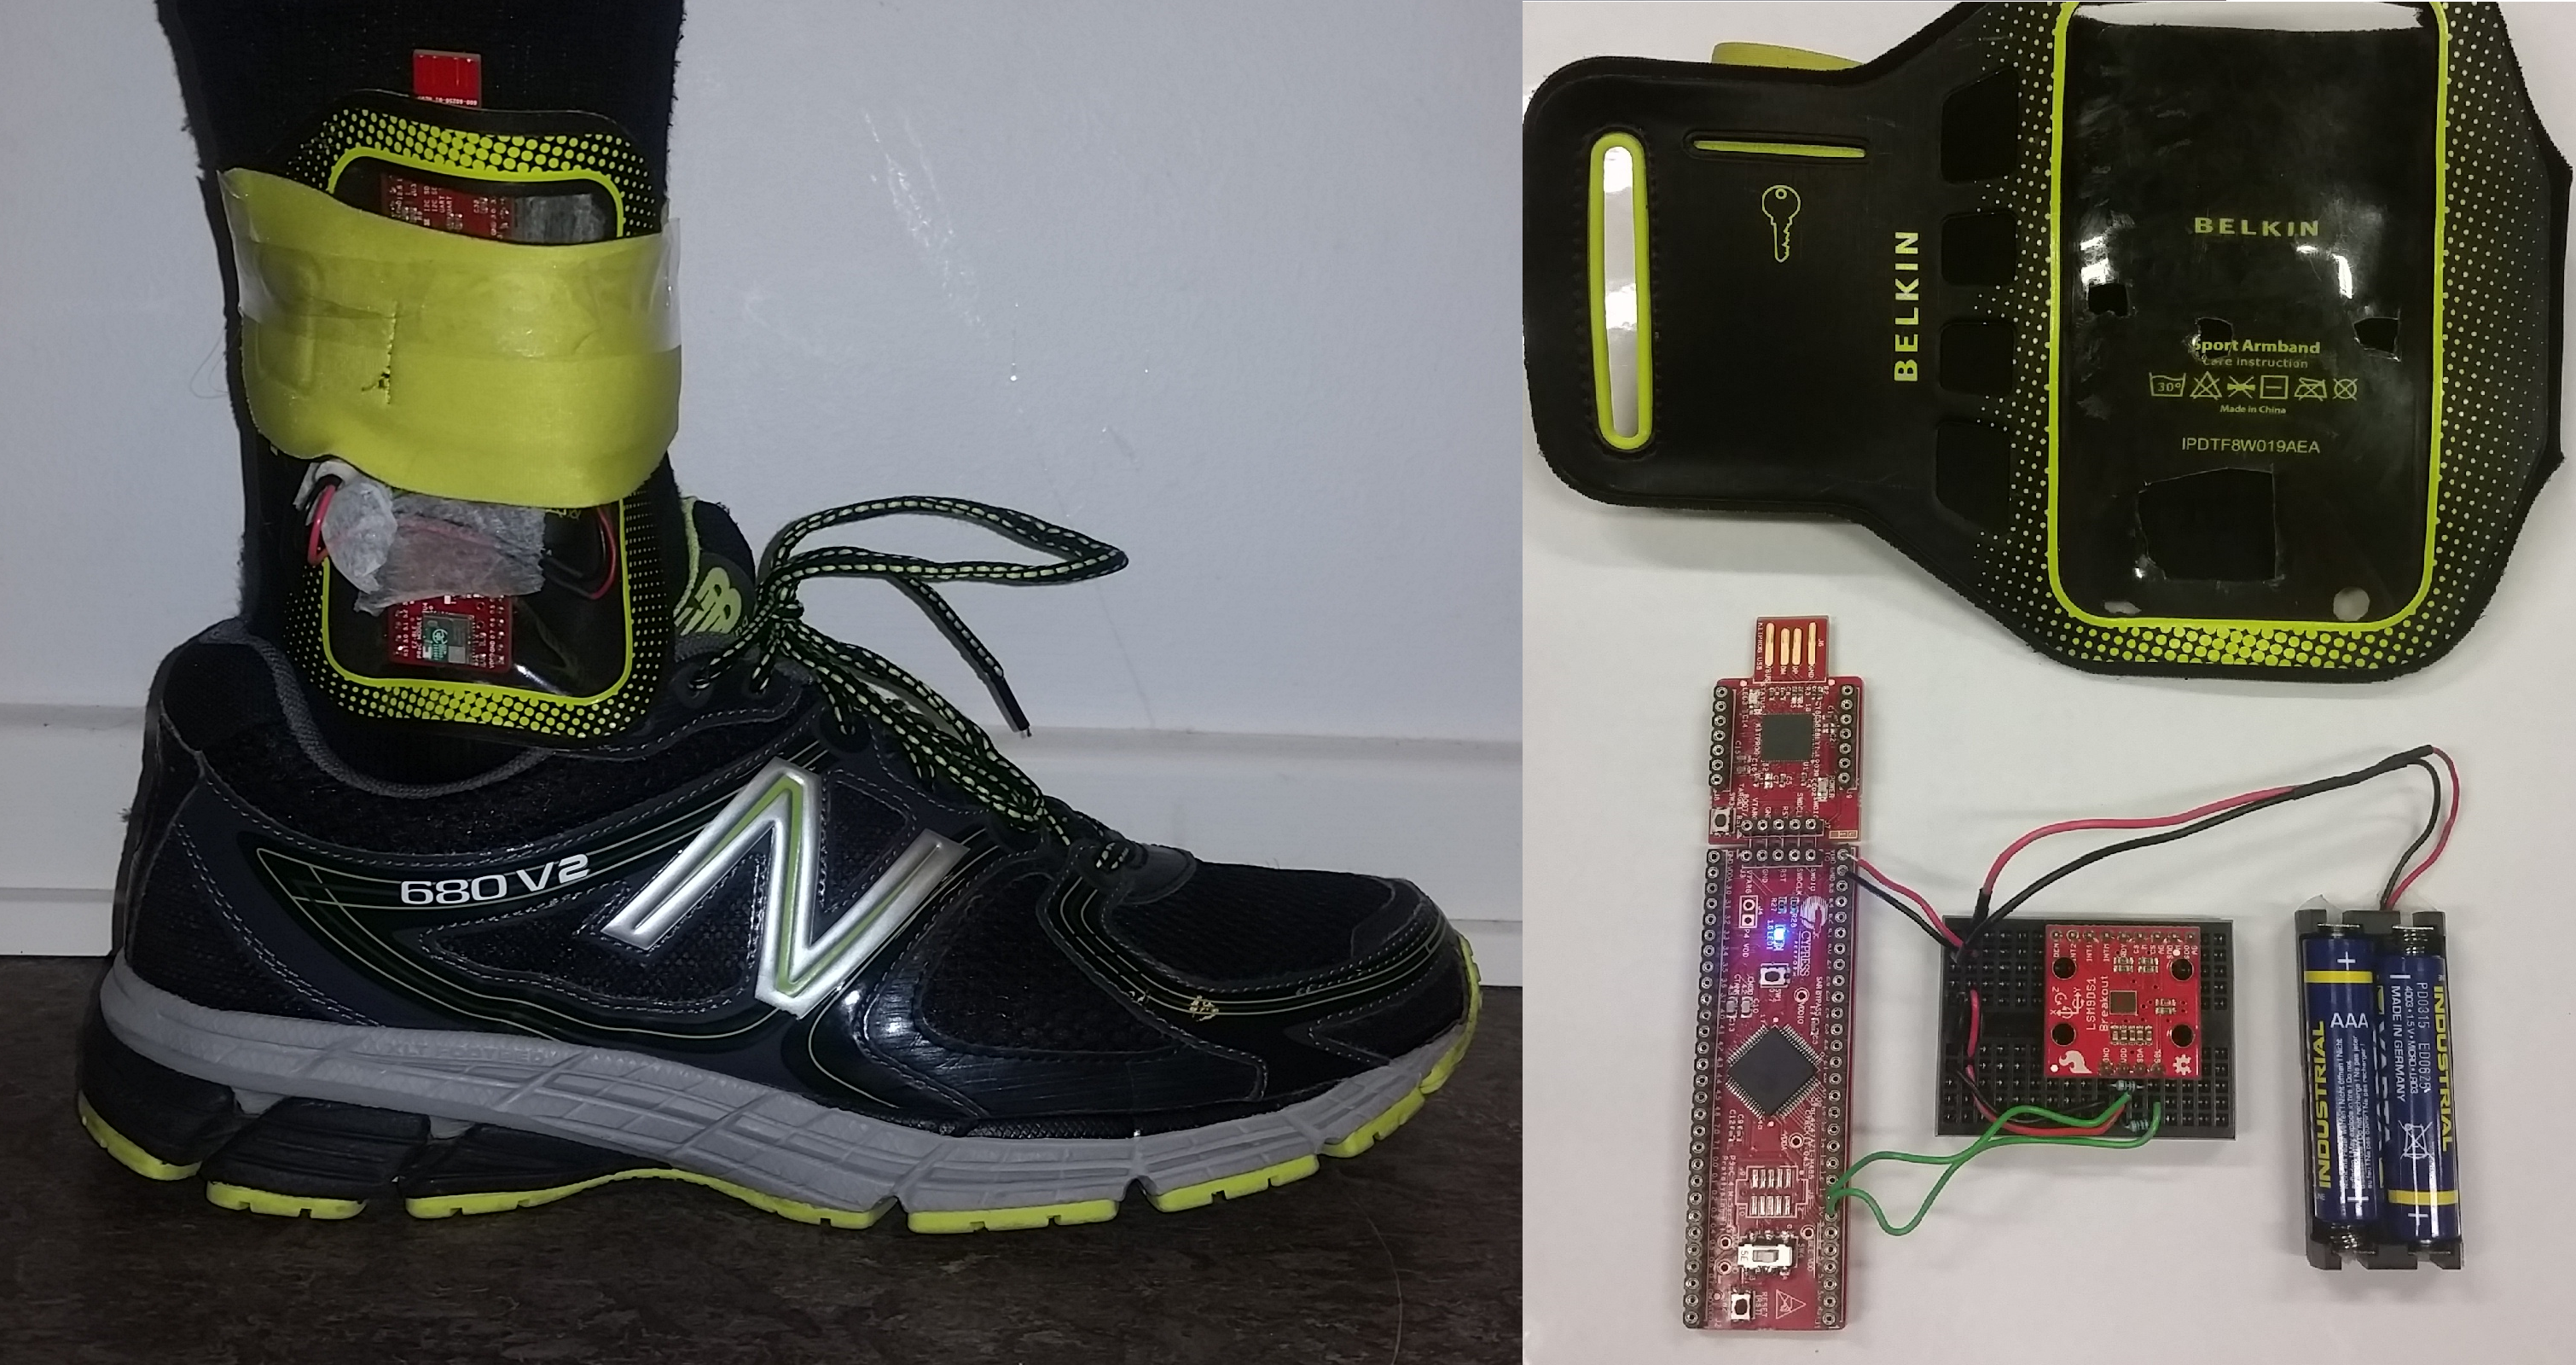
\includegraphics[scale=0.143]{figures/cDesign/samlet_system_paafod3.png}
	\caption{På figuren ses henholdsvis opsætningen af det endelige system på en forsøgsperson samt det samlede system taget ud fra opsætningen. Der ses, at EZ\_BLE modulet er frit tilgængeligt i bunden båndet til venstre i selve opsætningen.}
	\label{fig:samlede_system_opstilling}
\end{figure}

Ved test af det samlede system skal en forsøgsperson udføre tre aktiviteter: gang med 4,8 km/t, løb med 11,3 km/t og cykling med 20,9 km/t. Hver aktivitet skal udføres i 60 sekunder, og dataopsamlingen skal påbegyndes, når forsøgspersonen vurderer at have en homogen cyklus. Forinden tages en 60 sekunders måling, hvor forsøgspersonen står stille på løbebåndet. Det antages, at GUIen herved ikke vil optage nogen aktivitet. Fremgangsmåden for første test af systemet med gang ses herunder: 
\begin{itemize}
	\item GAP central og peripheral skal opdateres med korrekt algoritme på begge 4200M og EZ\_BLE mikroprocessorer.
	\item GAP peripheral med IC og en spændingsforsyning skal placeres proximalt for den laterale malleolus.
	\item GAP central kobles til en PC. 
	\item Forsøgspersonen skal stå oprejst med ret ryg, kigge ligeud og fødderne placeret parallelt på løbebåndet under 60 sekunders måling uden fysisk aktivitet.
	\item Herefter indstilles løbebåndet til en hastighed på 4,8 km/t. Forsøgspersonen går på løbebåndet indtil en homogen cyklus er opnået.  
	\item Et stopur startes samtidig med GUI, hvorved datastreaming fra GAP peripheral visualiseres på PCen.
	\item Dataopsamlingen skal foregå i 60 sekunder ifølge stopuret, hvorefter der trykkes på Q i MATLAB. Dette fryser figuren, således værdierne ved 60 skunder kan aflæses.
	\item Målingen stoppes.
\end{itemize}
Denne fremgangsmåde gentages to gange, hvor anden test er for detektion af løb og tredje test er for detektion af cykling. Forsøgspersonen dog sidder på en motionscykel under detektion af cykling. Resultatet fra denne test fremkommer som en fordeling af aktiviteter på GUIen, der helst ikke skal opfange aktivitet under målingen med ingen fysisk aktivitet. \\
Resultatet fra de forskellige tests ses i \tabref{tab:samlet_sys_test1}
\begin{table}[H]
	\centering
	\begin{tabular}{cccccc}
			\cellcolor[HTML]{C0C0C0}\begin{tabular}[c]{@{}c@{}} Udført\\aktivitet \end{tabular} & 	\cellcolor[HTML]{C0C0C0} Forsøgsperson & 	\cellcolor[HTML]{C0C0C0}\begin{tabular}[c]{@{}c@{}} Detektion af \\ gang {[}Sek{]} \end{tabular} & 	\cellcolor[HTML]{C0C0C0}\begin{tabular}[c]{@{}c@{}} Detektion af \\ løb {[}Sek{]} \end{tabular} & \cellcolor[HTML]{C0C0C0}\begin{tabular}[c]{@{}c@{}} Detektion af \\ cykling {[}Sek{]} \end{tabular} & \cellcolor[HTML]{C0C0C0}\begin{tabular}[c]{@{}c@{}} Afvigelse\\{[}\%{]} \end{tabular} \\ \hline
        \multirow{5}{*}{Gang}                                                     & 1             & 39,9                                                                                                & 1,1                                                                                              & 0  & 2,76                                                                                                   \\
		& 2             & 40,6                                                                                                & 0                                                                                                & 0   & 0                                                                                                  \\
		& 3             & 39                                                                                                  & 2                                                                                                & 0       & 5,13                                                                                              \\
		& 4             & 39,7                                                                                                & 1,6                                                                                              & 0      & 4,03                                                                                               \\
		& 5             & 40,8                                                                                                & 0                                                                                                & 0      & 0                                                                                               \\ \hline
		\multirow{5}{*}{Løb}                                                      & 1                                                                                                          & 1,2 & 39,9                                                                                             & 0     & 3,01                                                                                                \\
		& 2                                                                                           & 1,8  & 39                                                                                            & 0         & 4,62                                                                                            \\
		& 3                                                                                              & 0    & 40,8                                                                                            & 0      & 0                                                                                               \\
		& 4                                                                                                      & 0,4  & 40,4                                                                                            & 0     & 0,99                                                                                                \\
		& 5                                                                                                    & 0     & 40,6                                                                                           & 0         & 0   \\ \hline
		\multirow{5}{*}{Cykling}     & 1     & 0        & 0     & 40    & 0      \\
		& 2             & 0                                                                                                & 0                                                                                                & 40,1       & 0                                                                                              \\
		& 3             & 0                                                                                                  & 0                                                                                                & 40      & 0                                                                                              \\
		& 4             & 0                                                                                                  & 0                                                                                                & 40    & 0                                                                                                 \\
		& 5             & 0                                                                                                  & 0                                                                                                & 36 & 0   \\ \hline                                                                                                
		\end{tabular}
		\caption{I tabellen ses resultaterne fra de tre tests af det samlede system. Derudover er afvigelsen for hver detektion af fysisk aktivitet blevet udregnet.}
		\label{tab:samlet_sys_test1}
\end{table}{-0.5cm}
Der ses i \tabref{tab:samlet_sys_test1}, at GUIen optager mest gangsignal under gang, mest løbesignal under løb og udelukkende signal for cykling, når forsøgspersonen cyklede. Det fremgår ikke af tabellen, men for hver forsøgsperson ved stilstående måling blev der ikke detekteret nogen aktivitet af GUIen. \\
Den største afvigelse i detektion af den bestemte aktivitet er på 5,13\%. Dermed overholder systemet kravet om, at der må være en maks afvigelse på 10\%. Der ses dog også i \tabref{tab:samlet_sys_test1}, at GUIen detekterer cirka 40 sekunders data $pm$1 sekund, selvom dataopsamlingen varer i 60 sekunder. Dette vurderes imidlertid ikke være en faktor, der gør, at systemet vurderes til at være ikke funktionel, da samtlige krav undtagen pulsdetektering opfyldes. Årsagen til at systemet tilsyndeladende ikke sampler en tredjedel af signalet vil blive forklaret og diskuteret i \secref{sec:diskussion}.

Der foretages yderligere en test af systemet, hvor forsøgspersonerne først skal forsøge at gå ved en bestemt hastighed og derefter løbe ved samme hastighed. Derved testes systemet ved en hastighed, som både kan være gang og løb for at undersøge dets reaktion herfra. Fremgangsmåden for dette forsøg fremgår herunder:
\begin{itemize}
	\item GAP central og peripheral skal opdateres med korrekt algoritme på begge 4200M og EZ\_BLE mikroprocessorer.
	\item GAP peripheral med IC og en spændingsforsyning skal placeres proximalt for den laterale malleolus.
	\item GAP central kobles til en PC. 
	\item Forsøgspersonen skal forsøge at gå på løbebåndet med 8 km/t. 
	\item Når en homogen cyklus er opnået, startes et stopur samtidig med GUI, hvorved datastreaming fra GAP peripheral visualiseres på PCen.
	\item Dataopsamlingen skal foregå i 60 ifølge stopuret, hvorefter der trykkes på Q i MATLAB. Dette fryser figuren, således værdierne ved 60 sekunder kan aflæses.
	\item Målingen stoppes.
\end{itemize}
Denne fremgangsmåde testes yderligere, hvor forsøgspersonen skal løbe ved samme hastighed. 8 km/t er valgt på baggrund af pilotforsøget samt litteratur. I pilotforsøget skiftede hver forsøgsperson fra gang til løb under hastighedsstigningen mellem 8 og 20 km/t. Derudover hævder litteratur, at 4 miles per hour (mph) svarer til rask gang mens 6 mph er langsomt løb. 5 mph er cirka 8 km/t, hvilket understøtter valget af hastigheden. \citep{Miles2007} Resultatet fra denne test ses i \tabref{tab:samletsys_8kmt}
\begin{table}[H]
	\centering
	\begin{tabular}{cccccc}
		\cellcolor[HTML]{C0C0C0}\begin{tabular}[c]{@{}c@{}} Udført aktivitet \\ med 8 km/t\end{tabular} & 	\cellcolor[HTML]{C0C0C0} Forsøgsperson & 	\cellcolor[HTML]{C0C0C0}\begin{tabular}[c]{@{}c@{}} Detektion af \\ gang {[}Sek{]} \end{tabular} & 	\cellcolor[HTML]{C0C0C0}\begin{tabular}[c]{@{}c@{}} Detektion af \\ løb {[}Sek{]} \end{tabular} & \cellcolor[HTML]{C0C0C0}\begin{tabular}[c]{@{}c@{}} Detektion af \\ cykling {[}Sek{]} \end{tabular} & \cellcolor[HTML]{C0C0C0}\begin{tabular}[c]{@{}c@{}} Afvigelse\\{[}\%{]} \end{tabular} \\ \hline 
		\multirow{5}{*}{Gang}                                                     & 1             & 36,3                                                                                                & 4,3                                                                                              & 0  & 11,85                                                                                                   \\
		& 2             & 31,1                                                                                                & 9,9                                                                                                & 0   & 31,83                                                                                                  \\
		& 3             & 2,3                                                                                                  & 38,3                                                                                                & 0       & 94,3                                                                                              \\
		& 4             & 4                                                                                                & 36,7                                                                                              & 0      & 90,17                                                                                               \\
		& 5             & 0,4                                                                                                & 40,4                                                                                                & 0      & 99,02                                                                                               \\ \hline
		\multirow{5}{*}{Løb}                                                      & 1                                                                                                          & 0,8 & 40                                                                                             & 0     & 2                                                                                                \\
		& 2                                                                                           & 0,9  & 40                                                                                            & 0         & 2,25                                                                                            \\
		& 3                                                                                              & 2,3    & 38,6                                                                                            & 0      & 5,96                                                                                               \\
		& 4                                                                                                      & 0,2  & 40,7                                                                                            & 0     & 0,49                                                                                                \\
		& 5                                                                                                    & 0,9     & 40,2                                                                                           & 0         & 2,24   \\ \hline 
		\end{tabular}
	\caption{I tabellen ses resultaterne fra en test, hvor forsøgspersonerne skulle henholdsvis gå eller løbe ved samme hastighed. Der ses yderligere, at afvigelserne ved en mellemting mellem gang og løb er betydeligt mere signifikante, end ved klar gang eller løb. Dette går især ud over detektering af aktiviteten gang.}
	\label{tab:samletsys_8kmt}
\end{table}{-0.5cm}
Der ses i \tabref{tab:samletsys_8kmt}, at når tempoet for aktiviteten ikke er klar gang eller løb for forsøgspersonen, så vil den procentvise fordeling stige meget drastisk for gang data. Dette grunder i, at 8 km/t vurderes som værende meget rask gang fra hver forsøgsperson. Derfor vil g påvirkningen af accelerometerets y akse også blive påvirket med mere kræft end ved langsom gang. Der ses, at forsøgsperson 1 og 2 har lavere afvigelse for gangsignalet end forsøgsperson 3 til 5. Dette kan skyldes, at forsøgsperson 1 og 2 er mænd mens 3 til 5 er kvinder, hvor mændene er højere end kvinderne, har derved længere ben og muligvis en anden gangart end kvinderne. Dette diskuteres ligeledes i \secref{sec:diskussion}.

Afslutningsvis testes spændingsforbruget af den eksterne spændingsforsyning, som beskrevet i \secref{spaendingsforsyning}. Dette gøres nu, da en test heraf kræver, at systemet er samlet og under brug for at give en mere realistisk måling. Testen foregik således, at den eksterne spændingsforsyning fik udskiftet batterier og herefter målt outputspændingsniveauet. Efterfølgende blev spændingsforbruget målt hver halve time under samlet systemtest. Der antages, at spændingsforbruget er lineært faldende, hvorfor en gennemsnitsværdi for forbrug per time udregnes. \\
Spændingsforsyningen leverede 3,19 V fra starten af testen. Resultatet af de efterfølgende fem målinger ses i \tabref{tab:samlet_sys_batteri}
\begin{table}[H]
	\centering
	\begin{tabular}{cccc}
		\hline
		\cellcolor[HTML]{C0C0C0}Måling & \cellcolor[HTML]{C0C0C0}\begin{tabular}[c]{@{}c@{}} Spændingsniveau 1 time\\ inden måling {[}V{]} \end{tabular} & \cellcolor[HTML]{C0C0C0}\begin{tabular}[c]{@{}c@{}} Nuværende \\ spændingsniveau {[}V{]} \end{tabular} & \cellcolor[HTML]{C0C0C0}Spændingsforbrug {[}V{]} \\ \hline
		1 & 3,19 & 3,104 & 0,086 \\ \hline	
		2 & 3,104 & 3,052 & 0,052 \\ \hline	
		3 & 3,052 & 3,016 & 0,036 \\ \hline
		4 & 3,016 & 2,969 & 0,047 \\ \hline
		5 & 2,969 & 2,951 & 0,018 \\ \hline
	\end{tabular}
	\caption{I tabellen ses resultatet fra målingerne af spændingsforbruget for den eksterne spændingsforsyning. Der ses yderligere det beregnede spændingsforbrug for hver måling.}
	\label{tab:samlet_sys_batteri}
\end{table}\vspace{-0.5cm}
I \tabref{tab:samlet_sys_batteri} ses spændingsforbruget over fem målinger med en halv times interval. Da det antages, at spændingsforbruget har et lineært forhold, bliver en gennemsnit beregnet i \eqref{eq:samlet_sys1}
\begin{equation}
\frac{0,086 + 0,052 + 0,036 + 0,047 + 0,018}{5} \cdot 2 = 0,0956~V
\label{eq:samlet_sys1}
\end{equation}
Med antagelse af lineært forhold vil spændingsforsyningen falde med 0,0956 V per time. Da startspændingen var 3,19 V og den endelige spænding, hvormed MCUen ikke længere er funktionel, er 1,71 V, må det maksimale forbrug være $3,19 - 1,71 = 1,48$ V. Derfor er levetiden for den eksterne spændingsforsyning udregnet til:
\begin{equation}
\frac{1,48}{0,0956} = 15,481~timer.
\label{eq:samlet_sys2}
\end{equation}
I \eqref{eq:samlet_sys2} ses det, at den eksterne spændingsforsyning teoretisk kan få det samlede sytem til at være funktionel i 15,481 timer. Derfor overholder det samlede system kravet om, at det skal besidde batterilevetid for en hel dag svarende til 15 timer.
%
%
%\begin{table}[H]
%	\centering
%	\begin{tabular}{ccccc}
%		\hline
%		\rowcolor[HTML]{C0C0C0} 
%		Udført aktivitet & \begin{tabular}[c]{@{}c@{}} Detektion \\ af gang {[}Min{[} \end{tabular} & \begin{tabular}[c]{@{}c@{}} Detektion\\ af løb {[}Min{[}\end{tabular} & \begin{tabular}[c]{@{}c@{}} Detektion \\ af cykling {[}Min{[}\end{tabular} & y \\ \hline
%		Gang & 0 & 100 & 0 & 100 \\ \hline
%		Løb & 0 & 100 & 0 & 0 \\ \hline
%		Cykling & 0 & 0 & 100 & 0 \\ \hline
%	\end{tabular}%
%\end{table}\vspace{-.5cm}
%
%Der ses i \tabref{tab:samlet_sys_test1}, at systemet ikke detekterer gang korrekt. Det antages at være i forbindelse med tærskelværdierne, der adskiller gang og løb. Data fra Shimmer skal multipliceres med 16 for at give samme output, som data fra ICen, hvilket fremgår i \secref{sec:algogangloeb}. Der findes dog ikke samme forhold efter databehandlingen, hvorfor tærskelværdierne ikke blot kan multipliceres med 16. Derfor fortages endnu test, hvor målingerne skal ske ved konstant hastighed for henholdsvis gang og løb for at undersøge maksimal peak værdier. Derudover skal GAP peripheral kun sende data fra accelerometret, hvilket visualiseres i Realterm ved hjælp af GAP central. Algoritmen på GAB peripheral reguleres altså således, at gyroskopets data ikke sendes via BLE og tidsenheden imellem maks peaks er i dette tilfælde relevant. Der ønskes udelukkende en værdi for detekteringen af maks peak. Fremgangsmåden for denne test forekommer således:
%\begin{itemize}
%		\item GAP central og peripheral skal opdateres med korrekt algoritme på begge 4200M og EZ\_BLE mikroprocessorer.
%		\item GAP peripheral med IC og en spændingsforsyning skal placeres proximalt for den laterale malleolus.
%		\item GAP central kobles til en PC. 
%		\item En test af forbindelsen imellem GAP central og peripheral testes ved brug af Realterm på PCen.
%		\item Løbebåndet indstilles til 4,8 km/t. Forsøgspersonen går på løbebåndet indtil en konstant hastighed er opnået.
%		\item Realterm skal herefter visualisere data i 30 .
%		\item Målingen stoppes
%\end{itemize}
%Samme test fortages, hvor løbebåndet indstilles til 11,3 km/t. Data fra realterm konverteres, således Matlab kan genkende datatypen, hvorved en gennemsnitsværdi beregnes. Resultatet af disse to tests ses i \tabref{tab:samlet_sys_regulering}
%\begin{table}[H]
%	\centering
%	\begin{tabular}{cc}
%		\hline
%		\rowcolor[HTML]{C0C0C0} 
%		Aktivitet & \begin{tabular}[c]{@{}c@{}} Gennemsnitsværdi \\ for maks peak \end{tabular} \\ \hline
%			Gang & ? \\ \hline
%			Løb & ? \\ \hline
%		\end{tabular}%
%		\caption{I tabellen ses resultatet fra reguleringstesten for accelerometerdata.}
%		\label{tab:samlet_sys_regulering}
%\end{table}\vspace{-.5cm}
%Der ses i \tabref{tab:samlet_sys_regulering}, at maks peak værdierne for gang er langt højere, end værdierne var ved brug af Shimmer sensoren. Tærskelværdien for gang er 50, mens den for løb er 400. Disse skal reguleres, hvorefter det antages at algoritmen er tilpasset ICen. Ud fra værdierne fra \tabref{tab:samlet_sys_regulering} vælges de regulerede tærskelværdier til henholdsvis ? og ?. De nye tærskelværdier fremgår i \tabref{tab:samlet_sys_regulering2}.
%\begin{table}[H]
%	\centering
%	\begin{tabular}{ccc}
%		\hline
%		\rowcolor[HTML]{C0C0C0} 
%		Aktivitet & Gammel tærskelværdi & Reguleret tærskelværdi \\ \hline
%		Ingen aktivitet &  x~$\textless$~50 & ? \\ \hline
%		Gang & 50~$\textless$~x~$\textgreater$~400 & ? \\ \hline
%		Løb & 400~$\textgreater$~x & ? \\ \hline
%	\end{tabular}%
%	\caption{I tabellen ses resultatet fra reguleringstesten for accelerometerdata.}
%	\label{tab:samlet_sys_regulering2}
%\end{table}\vspace{-.5cm}
%Dette korrigeres inde i algoritmedesignet. Herefter fortages de tre seperate tests igen for det samlede system. Resultatet heraf ses i \tabref{tab:samlet_sys_test2}.
%\begin{table}[H]
%	\centering
%	\begin{tabular}{ccccc}
%		\hline
%		\rowcolor[HTML]{C0C0C0} 
%		Test nummer & \begin{tabular}[c]{@{}c@{}} Detektion \\ af gang {[}\%{[} \end{tabular} & \begin{tabular}[c]{@{}c@{}} Detektion\\ af løb {[}\%{[}\end{tabular} & \begin{tabular}[c]{@{}c@{}} Detektion \\ af cykling {[}\%{[}\end{tabular} & \begin{tabular}[c]{@{}c@{}} Afvigelse {[}\%{[} \end{tabular} \\ \hline
%			1 & 100 & 0 & 0 & 0 \\ \hline
%			2 & 0 & 100 & 0 & 0 \\ \hline
%			3 & 0 & 0 & 100 & 0 \\ \hline
%		\end{tabular}%
%		\caption{I tabellen ses resultaterne fra de tre tests af den anden samlede test af systemet. Der ses, at detektionen af den specifikke aktivitet er mere præcis efter reguleringen af tærskelværdierne.}%mhandlede revurdering af algoritmens tærskelværdier, samt vurdering af pulssensor.}
%		\label{tab:samlet_sys_test2}
%\end{table}\vspace{-.5cm}
%Det ses i \tabref{tab:samlet_sys_test2}, at systemet overholder kravet om en maksimal afvigelse på 10\% i forhold til fejlvurdering af aktivitet. \textbf{kog noget mere på det her, når vi har testet}.
%
%Systemet testes ligeledes for batteriets levetid. %, med henblik på at af,- eller bekræfte kravet vedrørende at kunne være batteridrevet igennem en hel dag. 
%Systemets initialeres til at starte samtidig med et stopur. Det samlede systems spændingsforsyning tilkobles et multimeter for at kunne måle dets spænding inden forsøget. Systemet skal køre uafbrudt i en time, hvorefter spændingsforsyningens igen tilkoples et multimeter og måles igen. 
%\begin{table}[H]
%	\centering
%	\begin{tabular}{cc}
%		\hline
%		\rowcolor[HTML]{C0C0C0} 
%		Spændingsniveau før forsøg {[}V{]} & Spændingsniveau efter forsøg {[}V{]} \\ \hline
%		3,14 & ????2,78???? \\ \hline
%	\end{tabular}
%	\caption{I tabellen ses testresultaterne vedrørende det samlede systems spændingsforbrug.}
%	\label{tab:test_spaending}
%\end{table} \vspace{-.5cm}
%Ud fra ovenstående testresultater beregnes der, at det samledes system forbruger 0,36 V per time. På baggrund i design af sensoren LSM9DS1 vides der, at den minimale tilførte spænding for funktionalitet af sensoren er 2,40 V. Dette resulterer systemet kan forbruge 0,74 V fra start, hvorefter systemet ikke forventes at fungere mere. 
%
%\begin{equation}
%Varighed~vedr\text{ø}rende~line\text{æ}r~operation = \frac{0,74~V}{0,36~V~per~time} = 2,05~timer
%\end{equation}   
%Det samlede system vil efter 2,05 timer have opbrugt tilpas spænding, således sensoren ikke længere er funktionel. % have opbrugt det spændingsarbejdsområde, hvoraf sensoreren opererer lineært. 
%Test af systemets levetid per batteri afkræfter dermed kravet heraf.
%
%Det samlede systems krav vedrørende et komfortabelt produkt for brugeren, samt bestå af et motiverende element for børn i aldersgruppen 9-12 år, blev ikke implementeret. Dette blev ikke implementeret, da systemet er en prototype, hvoraf fokus er på dets funktionalitet.  

\chapter{Syntese}
\section{Diskussion}\label{sec:diskussion}
%\textit{}

Indhold til diskussion i kort punktform:
\begin{itemize}
	\item Diskuter problemstillingen fra problemanalysen. Er det sundt og fornuftigt at gøre så unge mennesker bevidste om deres aktivitetsniveau og egen krop? Man kunne evt. kople lidt moderne livsstil ind over, hvor det er populært i vores moderne samfund at være fit og med på alle sociale medier (lidt langt ude...)
	\item Diskutter pilotforsøgets betydning for hele projektet. Hvorfor er der så stor forskel på de forskellige forsøgspersoners data? Hvilken betydning har denne spredning for hele designet af systemet? Var sensoren den mest optimale til forsøget? Hvis vi kunne lave noget om, hvad skulle det så være?
	\item Når der ikke tages højde for batterilevetid alligevel, havde det så ikke været en fordel at bruge gyroskop til detektering af alle aktiviteter, når dette signal var mere markant? 
	\item Havde almindelig bluetooth været bedre at benytte istedet for BLE? Hvilke andre muligheder havde det givet, både positiv (længere range) og negativ (kræver mere strøm)
	\item Diskutter at vores algoritme for cykling muligvis ikke tager højde for acceleration. Det er ikke noget vi kan sige med sikkerhed, da vi netop har tjekke for en fast hastighed. Vi mener, at under acceleration vil frekvenserne netop være fordelt mere end ved konstant hastighed - uanset hastighed - hvorved der muligvis kan forekomme fejl under acceleration.
	\item Tærskelværdien er ikke kalibreret. Dette Bliver over beskrevet i perspektiveringsafsnittet, hvordan dette kunne gøres - her kan man altså fokusere på, hvilken betydning har det for det samlede system?
	\item Hvis en person træder meget hårdt eller hopper meget under gang eller whatever og vedkommende får en værdi på eksempelvis 1500 under gang, så vil dette detekteres som løb. Hvad kan vi gøre for at løse dette?
	\item Diskussion om det samlede systemforsøg (der kommer sikkert til at være nogle diskussionselementer)
\end{itemize}

\section{Konklusion}
\textit{Følgende afsnit beskriver og konkluderer på projektets essentielle problemstillinger samt resultater. Afsnittet sammenholder projektets resultater med problemformuleringen, hvoraf en besvarelse præsenteres.}

Projektet beskriver udviklingen af en aktivitetsmåler, som har potentialet til at reducere antallet af fysisk inaktive børn i aldersgruppen 9-12 år. Systemet er bestående af algoritmer til detektering af aktiviteterne gang, løb og cykling. Systemets algoritmer er designet med hensigten at registrere disse specifikke fysiske aktiviteter, hvorefter resultaterne heraf benyttes som en motiverende faktor ved at visualisere tid og point. Aktiviteterne detekteres af henholdsvis et accelerometer og et gyroskop. Disse sensorer bidrager til detekteringen af den samlede udførte tid af hver aktivitet samt GUIs point system.

Systemet optræder mobilt i en grad, hvor trådløs dataoverførsel mellem GAP peripheral og GAP central er mulig. Ydermere er størstedelen af kravene til systemets delelementer opfyldt. Dette bidrager til, at det samlede system kan adskille og detektere aktiviteterne gang, løb og cykling ved benyttelse af de valgte sensorer. \\
Det samlede system kan tilnærmelsesvis automatisk detektere og adskille aktiviteterne. Under udførelsen af gang ved 4,8 km/t er alle forsøgspersonernes resultater tilnærmelsesvis ens, hvilket ligeledes afspejledes under løb samt cykling. Systemet overholder dermed kravet vedrørende en afvigelse på maksimalt 10\% i forhold til detektion af aktiviteterne. En tredjedel af de samlede samples detekteres ikke for samtlige forsøgspersoner og aktiviteter, hvorfor tidsenheden ikke angives korrekt. Dermed overholder systemet ikke det føromtalte krav med hensyn til afvigelse i varigheden. Dette medfører, at yderligere algoritme optimering er nødvendig, førend dette krav vil blive imødekommet til fulde.

Systemets funktionalitet bliver testet i GUI, hvor algoritmernes resultater visualiseres i form af aktiviteternes pointfordeling og varighed. Pulssensoren var tiltænkt at bidrage som en justerbar variabel til pointfordelingen, således et højt intensitetsniveau kan belønnes. Algoritmen hertil fungerer efter hensigten, men eftersom pulssensoren ikke leverer et korrekt output under udførsel af fysisk aktivitet, kan denne ikke accepteres. Pulssensoren skal derfor optimeres, førend en implementering i et endeligt system kan foregå. \\
Det samlede system har et gennemsnitligt spændingsforbrug på 0,0956~V per time med antagelsen om et lineært spændingsforbrug. Det samlede system vil med den benyttede spændingsforsyning antageligvis kunne operere i 8,3 timer, førend spændingsniveauet er under de tilladte 1,71~V. Det konkluderes hermed, at det samlede system ikke kan detektere og adskille aktiviteterne gang, løb og cykling optimalt i over 15 timer. 

På baggrund af testene af systemets delelementer samt testen af det samlede system kan det konkluderes, at systemet skal optimeres for at imødekomme alle funktionelle krav og herefter operere fuldstændigt efter hensigten. Hvis systemet bliver optimeret i en grad, hvor disse krav imødekommes, vil den udviklede aktivitetsmåler have potentialet til at kunne medvirke til en reduktion af fysisk inaktive børn i aldersgruppen 9-12 år. En optimering af systemet er en nødvendighed, hvormed der bør tages forbehold for at det udviklede system er en prototype. En videreudvikling af prototypen har potentialet til at indgå i et kommercielt samfundsmæssigt perspektiv.
\section{Perspektivering}
\textit{I dette afsnit bliver systemets funktionalitet sat i perspektiv. Systemets funktionalitet bliver vurderet i en grad hvor mulige optimeringsmetoder bliver undersøgt. Desuden beskrives der i perspektiveringen eventuelle videreudviklinger af det samlede system.}

Det nuværende system opfattes som en prototype, da opbygningen af det ikke anses som værende optimal. Systemet kan eksempelvis opbygges mere kompakt i forhold til hardware, således det er mere diskret. Det antages, at børn i den valgte aldersgruppe ikke ønsker, at systemet er tydeligt for andre, da hensigten ved brugen heraf er at mindske inaktivitet. Derfor ville det være optimalt, hvis systemet kan opbygges som et diskret bånd, der kan sidde på anklen uden det forekommer tydeligt for andre. For at dette kan lade sig gøre, kan systemet eventuelt benytte en mindre MCU, som har påmonteret accelerometer, gyroskop og pulssensor i én lille enhed, pulssensoren skal altså være en del af båndet omkring anklen og ikke sidde på øret. Det kræves at det samlede produkt har kontakt til huden, som resultat af dets implementerede pulssensor. Pulssensoreren er optisk og det kræves at denne er i kontakt med huden udfor en arterie, for at bestemme pulsen og heraf give en indikation omkring brugerens intensitetsniveau. Systemet anses mest optimalt placeret omkring anklen i et bånd, men en sekundær placering kunne være mulig. Førend en sekundær placering kunne inddrages ville en remodellering af systemets algoritmer og tærskelværdier være nødvendig. Algoritmen tilhørende detektering af cykling bør ydermere implementeres på MCUen, ligesom algoritmerne tilhørende gang og løb. Hvis dette bliver implementeret er det samlede system ikke begrænset i nogen grad med henblik på en eventuel GAP central i form af anden platform. MCUen vil uanset opbygning være nødvendig, da der skal fortages dataopsamling, databehandling og datakommunikation. Det kunne derudover være fordelagtigt, hvis den perifere MCU besidder mere RAM, således mere data kan gemmes herpå og ikke er afhængig af konstant overførsel af data. \\
BLE er en kommunikationsmulighed imellem den perifere og centrale enhed, dog har denne også sine begrænsninger i forhold til eksempelvis afstand. For optimal kommunikation kræver BLE, at enhederne er forholdsvis tæt på hinanden, hvilket kan være problematisk især for det nuværende system, da den centrale enhed består af en MCU tilkoblet en computer. En bruger kan derfor kun bevæge sig inden for en begrænset afstand herfra, da den perifere enhed sender data i realtid. En løsning heraf kunne enten være, at den perifere som sagt indeholder flere RAM eller at den centrale enhed bliver en app på en telefon, hvilket gør det samlede system mere mobilt. En anden løsning kunne være at implementere et 3G netværk i GAP peripheral, hvoraf data til enhver tid uploades til en online database. Uanset løsningen vil det være fordelagtigt at installere en alarm i form af enten en lysende LED eller lyd, som aktiveres i tilfælde af, at enhedernes kommunikation og dataoverførsel ikke er optimal og pakker bliver tabt. 

Resultatet af det samlede systems funktionalitet samt design, har denne et stort strømforbrug. Strømforbruget medfører at systemt ikke kan opererer over en hel dag. Dette er et resultat af flere årsager, bland andet omhandlende systemtes IC opsætning, algoritme og konstant dataoverførsel. Systemets IC er opsat til at opsamle data fra gyroskopet konstant. Gyroskopet er det delelement af ICen som har det største strømforbrug. En forbedring heraf ville bestå af en opsætning af ICen hvoraf der kun sendes når ny data, når ny data er tilgængelig. I mellemtiden går gyroskopet i søvntilstand, hvilket vil medføre at dets strømforbrug bliver reduceret kraftigt. Systemets algoritmer er et element hvis køretid bør undersøges hvorvidt en optimering er mulig. En reduktion i køretiden vil medføre at det samlede system kan gå i søvntilstand hurtigere og over længere tid, hvoraf strømforbruget ligeledes reduceres. Som nævnt tidligere ville en optimering af det samlede system bestå af en opgradering af dets RAM, hvilket kunne afhjælpe problematikken vedrørende konstant dataoverførsel. Ved opgradering af RAM vil systemets resultater kunne lagres, og sendes med længere mellemrum. Resultatet heraf ville medføre at systemets BLE modul kunne være i søvntilstand i længere tid end hidtil. En forbedring af ovenstående,  ville medføre en besparelse i systemets totale strømforbrug, og batteriets levetid ville blive forøget. Derved kan et mere strømbesparende system muligvis opnås.

Det samlede system benytter sig af et brugerinterface til illustration af dagens aktivitet. Dette brugerinterface er et element i denne prototype som kræver en optimering. Dette kan gøres mere brugervenligt og motiverende end den nuværende GUI. Herigennem kunne det være muligt at installere en brugervenlig kalibreringsenhed, hvor eksempelvis tærskelværdierne imellem gang og løb kan finindstilles til den individuelle bruger i stedet for at have en generel værdi. Dette vil gøre systemet mere præcist og pointværdierne for hver aktivitet vil uddeles mere korrekt. Ydermere bør brugerinterfacet indebære et motiverende spilelement, taget målgruppen i betragtning. Resultatet af at implementere et spil, bør motivere børnene til at være mere aktive end foruden det samlede system. Desuden vil det være muligt at lave et forældrelogin, hvorigennem forældre kan følge deres børns aktivitetsvaner og progression, det vil ligeledes være muligt for forældrene at motivere børnene igennem konkurrencer og fælles aktiviteter. Denne logintype kunne ligeledes gøres tilgængeligt for relevant sundhedspersonale\fxnote{eks. læge, sundhedsplejeske mm.}, hvilket kunne optimere deres grundlag for afhjælpning af eventuel inaktivitet og eller overvægt.

% - Pulsdata samplet med informationerne omkring den pågældende aktivitet kunne samles i systemet i en speciel fil, som ens læge kan få adgang til. Pulsen siger meget om kroppens fysiologiske tilstand. (Det er ret langt ude, så har ikke skrevet om det. Det vil virke lidt mærkeligt tror jeg)



\begingroup
\label{litteraturliste}
\raggedright
\bibliographystyle{unsrtnat}
\bibliography{kilder}
\endgroup

\begin{appendices}
	\chapter{Pilotforsøg}\vspace{-.75cm}\label{pilot}
\section{Formål}
Pilotforsøget udføres med henblik på at kunne designe algoritmer, som adskiller gang, løb og cykling. Det undersøges derudover, hvilke af accelerometerets og gyroskopets akser der er essentielle at lave algoritmer ud fra. Ydermere undersøges signalernes frekvens for at undgå aliasing i det endelige system. Sidst undersøges hvilken indflydelse placering af sensoren har på signalets udformning. Dette gøres, så det endelige systems signal ikke går i mætning på grund af for stor kraftpåvirkning, og for at undersøge om placering har indflydelse på signalernes udformning.

Til opsamling af data anvendes en Shimmer3. Dette er en enhed, som indeholder en række sensorer\fxnote{accelerometer, gyroskop, tryksensor, magnometer, højdemåler}, hvor der til forsøget benyttes et accelerometer og et gyroskop. 

Formålet med pilotforsøget er dermed:
\begin{itemize}
	\item At undersøge hvordan signalerne for gang, løb og cykling kan adskilles. 
	\item At undersøge hvilken betydning placering af sensorene har for signalets udformning ved gang, løb og cykling. 
	\item At bestemme frekvensområdet for signalerne.
	\item At bestemme amplituderne for signalerne.
\end{itemize}

\section{Metode}
Til forsøget medtages forsøgspersoner, som ikke lider af gener, der forhindrer dem i at udføre aktiviteterne gang, løb og cykling. Er en person skadet eller syg, eksluderes vedkommende dermed fra forsøget. Der udføres kun forsøg på gruppemedlemmer, og det er derfor ikke muligt at udføre forsøget på børn fra målgruppen, som er på 9-12 år. Resultaterne kan dermed eriere i forhold til målgruppen, da deres vægt og højde antages ikke at være tilserende forsøgspersonernes~\citep{Rigsholspitalet2014}. 

Forsøget tager udgangspunkt i tre forudbestemte placeringer på underbenet af enheden Shimmer3, hvilke kan ses på \figref{fig:sensor_placering}. Disse placeringer er udvalgt på baggrund af \secref{bevaegelse}, hvor det ses, at de største bevægelser optræder her i forbindelse med gang, løb og cykling. Accelerometeret registrerer position og acceleration, og det forventes derfor, at den største forskel vil kunne ses ved disse placeringer. I databehandlingen behandles kun data fra accelerometerets y-akse, da denne bør have den største kraftpåvirkning på baggrund af \secref{bevaegelse}.

\subsection{Materialer}
\begin{itemize}
	\item Løbebånd med justerbar hastighed og sikkerhedsbæresele.
	\item Motionscykel.
	\item Shimmer3 sensor med tilhørende holder og strap.
	\item Sportstape.
	\item Computer med følgende software:
	\begin{itemize}\vspace{-.15cm}
		\item Labview.
		\item Shimmer Sensing.
	\end{itemize}
\end{itemize}

\subsection{Fremgangsmåde}
Forsøgets fremgangsmåde er opdelt i to. Første del indeholder en opsætning af Shimmer3, mens den anden del er fremgangsmåden for optagelse af data fra forsøget.

\subsubsection{Opsætning af Shimmer3}
Før forsøgene kan udføres skal Shimmer3 forbindes korrekt med computeren og indstilles til at bruge de sensorer, der ønskes i pilotforsøget. \vspace{-3mm}
\begin{itemize}
	\item Shimmer3 forbindes til programmet Labview gennem bluetooth.
	\item Shimmer3 indeholder en række sensorer, hvoraf følgende skal aktiveres: 
	\begin{itemize}\vspace{-.15cm}
		\item Widerange Accelerometer.
		\item Gyroscope.
	\end{itemize}
	\item De maksimale arbejdsområder på $\pm$16~g og $\pm$2000~dps vælges, idet signalets amplitude endnu er ukendt.
	\item Samplingsfrekvensen indstilles på 512~Hz, da signalets frekvens er ukendt, og denne samplingsfrekvens er den maksimale der kan vælges, når både gyroskopet og accelerometeret er i brug.  
	\item Det er nu muligt at starte stream og derefter følge optagelserne i realtid.
\end{itemize}

\subsubsection{Udførsel af forsøget}
Forsøget udføres på fire forsøgspersoner, som alle skal udføre aktiviteterne gang, løb, hastighedsstigning og cykling. Den nedenstående beskrivelse af forsøgets fremgangsmåde er gældende for én af de forudbestemte placeringer af Shimmer3 på forsøgspersonens højre ben. Alle fire aktiviteter udføres før placeringen ændres, dog benyttes den samme fremgangsmåde til de resterende to placeringer. De tre placeringer kan ses på \figref{fig:sensor_placering}.
\begin{figure}[H]
	\centering
	\includegraphics[scale=0.55]{figures/qBilag/Sensor_placering2.png}
	\caption{På figuren ses hvor sensoren skal placeres under pilotforsøget. Placering A: proximalt for den laterale malleolus. Placering B: medialt på den laterale side af tibia. Placering C: distalt for patella på den laterale side. \citep{Perna2016,Shimmer2016} (Modificeret)}
	\label{fig:sensor_placering}
\end{figure}
Inden forsøget skal forsøgspersonen fastspændes i en sikkerhedssele, således der ikke opstår skader, hvis personen snubler på løbebåndet. Derudover skal forsøgspersonen inden hver måling fortælle, hvor på Borgskalaen vedkommende befinder sig, som kan ses på \figref{fig:borgskala}. Er dette under 11, kan målingen påbegyndes. Denne værdi er valgt for, at forsøgspersonen ikke foretager en aktivitet anderledes grundet muskeltræthed. Det sikres dermed, at alle forsøgspersoner har samme startbetingelser for alle forsøg. 
\begin{figure}[H]
	\centering
	\includegraphics[scale=0.35]{figures/qBilag/Borg-skala.jpg}
	\caption{På figuren ses Borgskalaen, som benyttes inden forsøgets start.~\citep{Patientinformationen2013} (Modificeret)}
	\label{fig:borgskala}
\end{figure}\vspace{-.25cm}

Første måling er gang, hvor hastigheden er 4,8~km/t og betegnes som værende en moderat hastighed~\citep{Miles2007}. %\vspace{-3mm}
\begin{itemize}
	\item Der foretages en baseline på 10~sekunder, hvor forsøgspersonen skal stå oprejst med ret ryg og fødderne placeret parallelt og kigge lige frem.
	\item Løbebåndet indstilles til 4,8~km/t, hvor forsøgspersonen går på løbebåndet indtil en konstant hastighed opnås. 
	%		\item Forsøgspersonen indikerer når denne føler en homogen bevægelses-cyklus.
	\item Målingen på 45~sekunder igangsættes.
\end{itemize}

Anden måling er løb, hvor hastigheden 11,3~km/t og betegnes som værende en energisk hastighed~\citep{Miles2007}. Fremgangsmåden for denne test er tilserende ovenstående fremgangsmåde for gang.

Tredje måling foretages på løbebåndet, hvor forsøgspersonen gradvist skal stige i tempo under hele forsøget. Der noteres under forsøget, hvornår forsøgspersonen skifter fra gang til løb.  %\vspace{-3mm}
\begin{itemize}
	\item Der foretages en baseline på 10~sekunder, hvor forsøgspersonen skal stå oprejst med ret ryg og fødderne placeret parallelt og kigge lige frem.
	\item Målingen igangsættes.
	\item Løbebåndet indstilles til 2~km/t, hvor forsøgspersonen skal gå i 20~sekunder.  
	\item Hastigheden stiger herefter med 2~km/t hvert 20. sekund, indtil forsøgspersonen har opnået sin vurderede maksimale hastighed, eller løbebåndets maksimale hastighed på 18~km/t opnås. 
	\item Målingen stoppes. 
\end{itemize}

Sidste måling fortages under cykling med en hastighed på 20,9~km/t, hvilket betegnes som værende et højt cykeltempo \citep{Miles2007}. Tempoet er dog underordnet, da der kun ønskes at se på forskellen i selve bevægelsen fra de andre aktivitetsformer, men der er valgt et fast tempo for at få et ensformigt signal. %\vspace{-3mm}
\begin{itemize}
	\item Der foretages en baseline på 10~sekunder, hvor forsøgspersonen skal sidde i en naturlig cykelposition på motionscyklen med begge fødder på pedalerne, hvoraf den højre pedal skal være helt i bund. Denne position er valgt, da den er mulig at lave tilnærmelsesvis ens for alle forsøgspersoner, hvormed de får den samme baseline.
	\item Forsøgspersonen træder i pedalerne, indtil vedkommende opnår en konstant hastighed på 20,9~km/t ved en belastning på 35~W. Dermed sikres det, at alle forsøgspersoner bruger den samme belastning gennem forsøget.  
	\item Målingen på 45~sekunder igangsættes. 
\end{itemize}
Efter de tre placeringer skulle forsøgspersonerne vurdere hvilken placering der er mest behagelig.

\section{Databehandling}
\subsection{Kalibrering af Shimmer3}
Forud for pilotforsøgets målinger blev Shimmer3 kalibreret og testet. For at undersøge hvorvidt kalibreringen af Shimmer3 fungerede optimalt, blev der opsamlet data til at be- eller afkræfte dette. Data fra de tre akser, x, y og z blev behandlet. \\
Når Shimmer3 er placeret i en kalibreringsboks på et bord med henblik på en respektiv akse, bør accelerometeret blive påvirket med $\pm$1~g, mens de resterende akser ikke bør påvirkes.
\begin{figure}[H]
	\centering
	\includegraphics[width=1\textwidth]{figures/qBilag/kalibreringsdata}
	\caption{På figuren ses kalibreringsdataene tilhørende accelerometerets x-, y- og z-akse.}
	\label{fig:Ap_Kalibrering}
\end{figure}
For hver akse udregnes den gennemsnitlige værdi for henholdsvis den positive- og negative akse og sammenholdes med $\pm 1$g. Dermed bestemmes blev den procentmæssige afvigelse fra tyngdeaccelerationen. Resultatet heraf ses i \tabref{fig:akser_pilot}
\begin{table}[H]
	\centering
	\begin{tabular}{ccc}		\hline
		\rowcolor[HTML]{C0C0C0} Akse & Positiv retning {[}\%{]} & Negativ retning {[}\%{]} \\ \hline
		x & 3,5 & -2,2 \\ \hline
		y & -0,6 & -2,6 \\ \hline
		z & 8,0 & 8,8 \\ \hline
	\end{tabular}
	\caption{I tabellen ses afvigelsen for hver af accelerometerets akser ved kalibrering.}
	\label{fig:akser_pilot}
\end{table}\vspace{-.25cm}
Kalibreringen foretages for at sikre, at et offset ikke er til stede. 

\subsection{Baseline for gang, løb og cykling}
Forud for hver enkelt måling foretages en baselinemåling som indikation for hvorvidt Shimmer3 fungerer forud for aktiviteten. Derudover benyttes baseline til at teste, hvorvidt Shimmer3 er i samme position for alle forsøgspersoner ved de forskellige målingers start. Dataene skal afspejle en tilnærmelsesvis fuldstændig tyngdekraftpåvirkning på accelerometerets y-akse, som resultat af Shimmer3s placering på benet. Baseline foretages for at sikre, at Shimmer3 tilnærmelsesvis bliver placeret ens på alle forsøgspersoner, hvormed data kan sammenholdes. 
\begin{table}[H]
	\centering
	\begin{tabular}{cccc}
		\hline
		\cellcolor[HTML]{C0C0C0} Forsøgsperson & \cellcolor[HTML]{C0C0C0}\begin{tabular}[c]{@{}c@{}}Placering A, \\ y-akse {[}g{]}\end{tabular} & \cellcolor[HTML]{C0C0C0} \begin{tabular}[c]{@{}c@{}}Placering B,\\ y-akse {[}g{]}\end{tabular} & \cellcolor[HTML]{C0C0C0} \begin{tabular}[c]{@{}c@{}}Placering C,\\ y-akse {[}g{]}\end{tabular} \\ \hline
		F1 & 0,98 & 0,99 & 0,97 \\ \hline
		F2 & 1 & 0,99 & 0,96 \\ \hline
		F3 & 0,98 & 0,98 & 0,98 \\ \hline
		F4 & 0,97 & 0,99 & 0,95 \\ \hline
	\end{tabular}
	\caption{I tabellen ses de gennemsnitlige baselineresultater fra accelerometerets y-akse forud for gang.}
	\label{fig:Ap_baselinegang}
\end{table}\vspace{-0.5cm}
\begin{table}[H]
	\centering
	\begin{tabular}{cccc}
		\hline
		\cellcolor[HTML]{C0C0C0} Forsøgsperson & \cellcolor[HTML]{C0C0C0} \begin{tabular}[c]{@{}c@{}}Placering A, \\ y-akse {[}g{]}\end{tabular} & \cellcolor[HTML]{C0C0C0} \begin{tabular}[c]{@{}c@{}}Placering B,\\ y-akse {[}g{]}\end{tabular} & \cellcolor[HTML]{C0C0C0} \begin{tabular}[c]{@{}c@{}}Placering C,\\ y-akse {[}g{]}\end{tabular} \\ \hline
		F1 & 0,99 & 0,99 & 0,97 \\ \hline
		F2 & 0,99 & 0,99 & 0,96 \\ \hline
		F3 & 0,97 & 0,98 & 0,98 \\ \hline
		F4 & 0,97 & 0,99 & 0,95 \\ \hline
	\end{tabular}
	\caption{I tabellen ses de gennemsnitlige baselineresultater fra accelerometerets y-akse forud for løb.}
	\label{fig:Ap_baselineloeb}
\end{table}\vspace{-0.5cm}

Ved cykling benyttes gyroskopets data, da cykling detekteres som en roterende bevægelse omkring z-aksen. Enheden af dataet heraf er dps, og dermed bør baselineresultaterne ligge omkring nul.
\begin{table}[H]
	\centering
	\begin{tabular}{cccc}
		\hline
		\cellcolor[HTML]{C0C0C0} Forsøgsperson & \cellcolor[HTML]{C0C0C0} \begin{tabular}[c]{@{}c@{}}Placering A, \\ z-akse {[}dps{]}\end{tabular} & \cellcolor[HTML]{C0C0C0} \begin{tabular}[c]{@{}c@{}}Placering B,\\ z-akse {[}dps{]}\end{tabular} & \cellcolor[HTML]{C0C0C0} \begin{tabular}[c]{@{}c@{}}Placering C,\\ z-akse {[}dps{]}\end{tabular} \\ \hline
		F1 & -0,98 & -0,83 & -0,87 \\ \hline
		F2 & -0,90 & -0,79 & -0,77 \\ \hline
		F3 & -0,68 & -0,58 & -0,99 \\ \hline
		F4 & -0,89 & -0,92 & -0,85 \\ \hline
	\end{tabular}
	\caption{I tabellen ses de gennemsnitlige baselineresultater fra gyroskopets z-akse forud for cykling.}
	\label{fig:Ap_baselinecykling}
\end{table}\vspace{-0.5cm}

\subsection{Minimum og maksimum g-påvirkning under gang, løb og hastighed}
Dataene fra aktiviteterne gang, løb og hastighedsstigning behandles med henblik på bestemmelse af den maksimale g-påvirkning heraf. Dette bliver bestemt af den maksimale påvirkning i henholdsvis accelerometerets positive og negative y-akse samt placeringer. Før forsøgene bestemmes baseline forinden hvert forsøg. 

Den største afvigelse fra tyngdeaccelerationen for gang er på 0,9969\%, hvormed det vurderes, at alle baselines er uden betydeligt offset.\Tabref{fig:Ap_maxggang} viser resultaterne fra gang med et hastighed på 4,8~km/t.
\begin{table}[H]
	\centering
	\begin{tabular}{cccc}
		\hline
		\rowcolor[HTML]{C0C0C0} 
		Forsøgsperson & \begin{tabular}[c]{@{}c@{}} Placering A {[}g{]}\end{tabular} & \begin{tabular}[c]{@{}c@{}} Placering B {[}g{]}\end{tabular} & \begin{tabular}[c]{@{}c@{}} Placering C {[}g{]}\end{tabular} \\ \hline
		F1 &  0,09 ; 2,51  & 0,00 ; 2,32  & -2,51 ; 3,33 \\ \hline
		F2 &  -0,19 ; 3,19 & -0,43 ; 3,04 & -0,97 ; 2,84 \\ \hline
		F3 &  -0,24 ; 3,52 & -0,39 ; 3,38 & -0,20 ; 2,51 \\ \hline
		F4 &  -0,04 ; 2,84 & -0,29 ; 3,62 & -0,50 ; 3,52 \\ \hline
	\end{tabular}%
	\caption{I tabellen ses de maksimale positive og negative værdier fra accelerometerets y-akse som resultat af gang med en hastighed på 4,8~km/t. Værdierne er fundet for både placering A, B og C.}
	\label{fig:Ap_maxggang}
\end{table}\vspace{-.25cm}
Det ses i \tabref{fig:Ap_maxggang}, at den maksimale g-påvirkning under gang for placering A er i intervallet -0,24~g til 3,52~g. Den maksimale g-påvirkning for placering B er i intervallet -0,43~g til 3,62~g mens den for C er -2,51~g til 3,52~g.

På samme måde findes baseline for løb ved en hastighed på 11,3~km/t, som maksimalt afviger med 0,9930\%. Det vurderes derfor, at baseline for alle forsøgspersoner inden løb er uden betydeligt offset. Herefter blev der fundet de maksimale positive og negative værdier for løb, som kan ses i \tabref{fig:Ap_maxgloeb}.  
\begin{table}[H]
	\centering
	\begin{tabular}{cccc}
		\hline
		\rowcolor[HTML]{C0C0C0} 
		Forsøgsperson & \begin{tabular}[c]{@{}c@{}} Placering A {[}g{]}\end{tabular} & \begin{tabular}[c]{@{}c@{}} Placering B {[}g{]}\end{tabular} & \begin{tabular}[c]{@{}c@{}} Placering C {[}g{]}\end{tabular} \\ \hline
		F1 &  -2,03 ; 8,59 & -2,80 ; 5,07 & -4,10 ; 3,33 \\ \hline
		F2 &  -0,97 ; 5,35 & -2,51 ; 6,13 & -4,44 ; 6,52 \\ \hline
		F3 &  -2,12 ; 5,55 & -1,83 ; 5,60 & -2,46 ; 5,60 \\ \hline
		F4 &  -3,48 ; 6,42 & -4,63 ; 6,76 & -3,52 ; 8,30 \\ \hline
	\end{tabular}%
	\caption{I tabellen ses de maksimale positive og negative værdier fra accelerometerets y-akse som resultat af løb med en hastighed på 11,3~km/t. Værdierne er fundet for både placering A, B og C.}
	\label{fig:Ap_maxgloeb}
\end{table}\vspace{-.25cm}
Det ses i \tabref{fig:Ap_maxgloeb}, at den maksimale g-påvirkning under gang for placering A er i intervallet -3,48~g til 4,59~g. Den maksimale g-påvirkning for placering B er i intervallet -4,63~g til 6,76~g mens den for C er -4,44~g til 8,30~g.

Afslutningsvis bliver accelerometerets y-akse undersøgt ved forsøget, hvor forsøgspersonerne gradvist stiger i tempo. Baseline for disse målinger afviger med 0,9954\%, hvormed det vurderes, at baseline for alle målinger er neutrale. Den maksimale påvirkning i henholdsvis positiv og negativ retning, som detekteres under hastighedsstigningen, kan ses i \tabref{fig:Ap_maxghastighed1} 
\begin{table}[H]
	\centering
	\begin{tabular}{cccc}
		\hline
		\rowcolor[HTML]{C0C0C0} 
		Forsøgsperson & \begin{tabular}[c]{@{}c@{}} Placering A {[}g{]}\end{tabular} & \begin{tabular}[c]{@{}c@{}} Placering B {[}g{]}\end{tabular} & \begin{tabular}[c]{@{}c@{}} Placering C {[}g{]}\end{tabular} \\ \hline
		F1 &  -3,04 ; 8,20  & -4.59 ; 6,28  & -6,66 ; 7,10 \\ \hline
		F2 &  -3,19 ; 10,96 & -4,49 ; 10,48 & -7,58  ; 9,61 \\ \hline
		F3 &  -4,92 ; 10,48 & -4,59 ; 13,13 & -4,63 ; 9,70 \\ \hline
		F4 &  -8,83 ; 16,95 & -7,48 ; 16,32 & -8,01 ; 15,35 \\ \hline
	\end{tabular}%
	\caption{I tabellen ses de maksimale positive og negative værdier fra accelerometerets y-akse som resultat af hastigheds stigning. Værdierne er fundet for både placering A, B og C.}
	\label{fig:Ap_maxghastighed1}
\end{table}\vspace{-.25cm}
Det ses i \tabref{fig:Ap_maxghastighed1}, at den maksimale g-påvirkning under gang for placering A er i intervallet -8,83~g til 16,95~g. Den maksimale g-påvirkning for placering B er i intervallet -7,48~g til 16,32~g mens den for C er -8,01~g til 15,35~g.

\subsection{Maksimal omdrejninger per sekund under cykling}
Dataene fra aktiviteten, cykling, behandles med henblik på bestemmelse af den maksimale amplitude fra gyroskopet. Dette bestemmes ved at beregne den maksimale peak-to-peak under udførelsen af cykling. Dataene behandles med henblik på gyroskopets z-akse som resultat af \secref{bevaegelse}. Inden dataopsamling for cykling måles en baseline. Den maksimale afvigelse fra en værdi på 0 er -0,9979\%, hvormed det vurderes, at alle målinger har en neutral baseline. Dataene fra forsøget kan ses i \tabref{fig:Ap_maxghastighed}.
\begin{table}[H]
	\centering
		\begin{tabular}{cccc}
			\hline
			\rowcolor[HTML]{C0C0C0} 
			Forsøgsperson & \begin{tabular}[c]{@{}c@{}} Placering A {[}dps{]}\end{tabular} & \begin{tabular}[c]{@{}c@{}} Placering B {[}dps{]}\end{tabular} & \begin{tabular}[c]{@{}c@{}} Placering C {[}dps{]}\end{tabular} \\ \hline
			F1 & -148,23 ; 108,29   & -209,82 ; 118,60   & -188,66 ; 98,29  \\ \hline
			F2 & -108,42 ; 108,11   & -133,11 ; 114,94	 & -150,43 ; 120,61 \\ \hline
			F3 & -208,29 ; 136,28  	& -196,95 ; 140,18	 & -195,43 ; 151,10 \\ \hline
			F4 & -182,56 ; 152,13  	& -159,82 ; 138,35	 & -152,62 ; 136,83 \\ \hline
		\end{tabular}%
	\caption{I tabellen ses de maksimale positive og negative værdier fra gyroskopets z-akse som resultat af cykling med en hastighed på 20,9 km/t. Værdierne er fundet for både placering A, B og C.}
	\label{fig:Ap_maxghastighed}
\end{table}\vspace{-.25cm}
Det ses i \tabref{fig:Ap_maxghastighed}, at den maksimale dps under gang for placering A er i intervallet -208,29~dps til 152,13~dps. Den maksimale g-påvirkning for placering B er i intervallet -209,82~dps til 140,18~dps mens den for C er -195,43~dps til 151,10~dps. 

\subsection{Afgrænsning af placering}
Databehandling tager udgangspunkt i de maksimale værdier fra placering A. Dette gøres på baggrund af, at denne er den mest optimale placering i forhold til komfort for brugeren, da tre ud af fire forsøgspersoner foretrak denne placering. Den maksimale værdi for placering A overskrider den maksimale accelerationskraftpåvirkning med 0,95 g. Det vurderes dog at placering A er optimal at bruge, da de 16,95~g repræsenteres i form af hælnedslag. Det vil stadig være muligt at adskille hælnedslag fra det resterende signal, selvom det vil klippes ved 16~g. \newline
Gyroskopets data viser ligeledes, at det er muligt at benytte placering A, da denne viser at cykling ikke resulterer i en høj dps. På baggrund af dette vil der i det resterende databehandling tages udgangspunkt i placering A, som kan ses i fem sekunders interval for hver af de fire forsøgspersoner på \figref{raa_data}.
\begin{figure}[H]
	\centering
	\includegraphics[width=1\textwidth]{figures/qBilag/raa_data}
	\caption{På figuren ses det ubehandlede data fra de tre aktivitetstyper gang, løb og cykling, hvoraf data for gang og løb er fra accelerometret mens data for cykling er fra gyroskopet ved placering A.}
	\label{raa_data}
\end{figure}\vspace{-.25cm}

\subsection{Frekvensindhold af gang, løb og cykling}
Dataene fra aktiviteterne gang og løb behandles for at bestemme signalernes frekvensindhold. Resultatet af dette muliggør bestemmelsen af samplingsfrekvensen vedrørende accelerometeret og gyroskopet. Der foretages en frekvensdomæne analyse, hvilket muliggør visualisering af signalets magnitude ved forskellige frekvenser, hvoraf energien af signalet kommer til udtryk.
\begin{figure}[H]
	\centering
	\includegraphics[width=1\textwidth]{figures/qBilag/fft_f1_loeb}
	\caption{På figuren ses frekvensdomænet af aktiviteten løb for forsøgsperson 1. Den fuldstændige magnitude for de lave frekvenser vises ikke til fulde. Hvis dette skulle være tilfældet ville de mindste magnituder på figuren blive udskalleret.}
	\label{fig:Ap_FFt}
\end{figure}\vspace{-.25cm}
Frekvensdomæneanalysen vises kun for løb af F1, da frekvensspektrummet er størst heraf. Derudover vises den ikke for gang, da denne ydermere er lavere end for løb, og da begge aktiviteter skal detekteres med et accelerometer, skal de have samme samplingsfrekvens. Dermed vises kun frekvensspektrummet for løb, da systemets samplingsfrekvens bestemmes i forhold til den højest målte frekvens.

Data fra aktiviteten, cykling behandles for at bestemme signalernes frekvensindhold, med henblik på bestemmelsen af samplingsfrekvensen vedrørende gyroskopet.
\begin{figure}[H]
	\centering
	\includegraphics[width=1\textwidth]{figures/qBilag/cykling_frekvens}
	\caption{På figuren ses frekvensdomænet af aktiviteten cykling for alle forsøgspersoner. Den fuldstændige magnitude for de lave frekvenser vises ikke til fulde. Hvis dette skulle være tilfældet ville de mindste magnituder på figuren blive udskalleret.}
	\label{fig:Ap_cyklingfrekvens}
\end{figure}\vspace{-.25cm}

\subsection{Accelerometer karakteristika vedrørende gang og løb}
Dataene fra aktiviteten gang og løb behandles med henblik på bestemmelse af signalets karakteristika, således en sammenligning og senere algoritmedesign muliggøres. Dataene fra accelerometerets y-akse blev for alle forsøgspersoner lavpasfiltreret ved 45~Hz grundet frekvensspektret på \figref{fig:Ap_FFt}. Derudover blev signalet differentieret, hvorved områderne med størst hældningskoefficient kommer til udtryk. Herigennem fremhæves hælnedslag og tåafsæt, idet disse events har en stor hældning.
\begin{figure}[H]
	\centering
	\includegraphics[width=1\textwidth]{figures/qBilag/gang_diff}
	\caption{På figuren ses det filtrerede og differentierede data fra aktiviteten gang for alle forsøgspersoner.}
	\label{fig:Ap_gangdiff}
\end{figure}\vspace{-.25cm}
Det ses på \figref{fig:Ap_gangdiff}, at hælnedslag og tåafsæt fremgår tydligere end på \figref{raa_data} for både gang og løb. Ydermere ses det på \figref{fig:Ap_loebdiff}, at amplituderne for hælnedslag og tåafsæt øges ved løb.
\begin{figure}[H]
	\centering
	\includegraphics[width=1\textwidth]{figures/qBilag/loeb_diff}
	\caption{På figuren ses det filtrerede differentierede data fra aktiviteten løb for alle forsøgspersoner.}
	\label{fig:Ap_loebdiff}
\end{figure}\vspace{-.25cm}

\subsection{Gyroskop karakteristika vedrørende gang, løb og cykling}
Dataene fra aktiviteterne gang, løb og cykling behandles med henblik på bestemmelse af signalets karakteristika. Dette udføres ved at sammensætte forsøgspersonernes data, således en sammenligning muliggøres. Aktiviteterne gang og løb behandles for at sikre dette ikke har tilsvarende karakteristika som cykling, med henblik på algoritmedesign. Dataene behandles med henblik på gyroskopets z-akse, som resultat af \secref{bevaegelse}. Dette kan ses på \figref{fig:Ap_cykling1}, \figref{fig:Ap_cykling2} og \figref{fig:Ap_cykling3}.
\begin{figure}[H]
	\centering
	\includegraphics[width=1\textwidth]{figures/qBilag/gang_gyro}
	\caption{På figuren ses dataene fra gang ved 4,8 km/t fra de fire forsøgspersoner. Dataene er fra gyroskopets z-akse.}
	\label{fig:Ap_cykling1}
\end{figure}\vspace{-.25cm}

\begin{figure}[H]
	\centering
	\includegraphics[width=1\textwidth]{figures/qBilag/loeb_gyro}
	\caption{På figuren ses dataene fra løb ved 11,3 km/t fra de fire forsøgspersoner. Dataene er fra gyroskopets z-akse.}
	\label{fig:Ap_cykling2}
\end{figure}\vspace{-.25cm}

\begin{figure}[H]
	\centering
	\includegraphics[width=1\textwidth]{figures/qBilag/cykling_gyro}
	\caption{På figuren ses dataene fra cykling ved 20,9 km/t fra de fire forsøgspersoner. Dataene er fra gyroskopets z-akse.}
	\label{fig:Ap_cykling3}
\end{figure}\vspace{-.25cm}

\section{Diskussion}
\subsection{Kalibrering af Shimmer3}
Resultatet af databehandlingen bevirker, at kalibreringen af Shimmer3 antages at være tilstrækkelig. Dette antages at være tilstrækkeligt, da y-aksen afviger med henholdsvis -2,6\% i den negative akse og -0,6\% i den positive akse fra den teoretiske værdi. En eventuel fejlkilde til at denne fejlmargin kan være, at bordet hvorpå Shimmer3 er placeret, ikke er helt i vatter.

\subsection{Baseline for gang, løb og cykling}
Baselinemålingerne for henholdsvis gang og løb resulterer i en sammenligning af påvirkningen. g-påvirkningen af Shimmer3 er ikke præcis 1~g under kalibrering, hvilket kan være et resultat af, at Shimmer3 ikke er placeret ortogonalt på y-aksen på benet. Idet Shimmer3 ikke er placeret ortogonalt på benet, kan der være opstået en mindre hældning, hvorfor y-aksen ikke påvirkes med præcist 1~g. Resultaterne fra disse målinger indikerer, at Shimmer3 har optaget data som stemmer overens med antagelsen om den tilnærmelsesvise påvirkning på 1~g. 

Resultaterne fra baselinemålingerne vedrørende cykling ligger som forventet omkring 0, hvilket er et resultat af, at Shimmer3 ikke er blevet påvirket i z-aksen i nogen væsentlig grad, da benet ikke bevæges. Resultaterne af disse målinger indikerer, at Shimmer3 har optaget data, som stemmer overens med antagelsen om den tilnærmelsesvise påvirkning på 0~dps\fxnote{maksimal afvigelse på -0,9979}. 

\subsection{Maksimal g-påvirkning under gang, løb og hastighed} \label{app:maxg}
Resultatet af databehandlingen vedrørende de tre aktiviteter med henblik på bestemmelsen af den maksimale g-påvirkning medfører, at aktiviteten med hastighedsstigning har den største påvirkning. Resultaterne fra placering A, B eller C fra F1, F2 og F3 overskrider ikke $\pm16$~g. Resultaterne fra F4 overskrider 16~g med 0,95~g. Dette vurderes dog til ikke at have en væsentligt betydning, hvoraf den mest fordelagtige placering vælges. Med baggrund i \secref{succeskrav} og \secref{funktionellekrav} skal placeringen ikke være til gene for barnet og skal nemt af- og påmonteres, hvoraf placering A er valgt, da denne vurderes som værende mest komfortabel blandt forsøgspersonerne. Dette medfører, at den videre resultatbehandling udelukkende tager udgangspunkt i placering A. 

\subsection{Maksimal omdrejninger per sekund under cykling}
Resultatet af databehandlingen vedrørende maksimal omdrejninger ved cykling resulterer i et spænd mellem 216,5~dps og 320,4~dps. Dette kan være et resultat af, at forsøgspersonerne ikke har holdt samme hastighed. En pludselig acceleration kan derfor muligvis give en ændring, som ikke er relateret til cykling ved 20,9~km/t. I takt med at der maksimalt bliver registreret 320,4~dps, er dette medbestemmende vedrørende valg af et endeligt gyroskop. Et gyroskop til det endelige system skal heraf have et arbejdsområde som er større end 320,4 dps, men det præcise arbejdsområde vides ikke, da en hastighedsstigning ikke blev foretaget for cykling.

\subsection{Frekvensindhold af løb og cykling}
Databehandlingen af frekvensindholdet fra gang og løb påviser, at det største frekvensspektrum er placeret mellem 0~Hz og 45~Hz. Dette medfører, at samplingsfrekvensen vedrørende data fra accelerometeret kan bestemmes. \\
Databehandling af frekvensindholdet fra cykling påviser, at det største frekvensspektrum ligger mellem 0~Hz og 6~Hz. Dette medfører, at samplingsfrekvensen vedrørende data fra gyroskopets kan bestemmes. 

\subsection{Accelerometer karakteristika vedrørende gang og løb}
Databehandlingen vedrørende accelerometerets karakteristika af gang og løb resulterer i en sammenligning af dataene. Dataene fra gang viser to events, hvor peaks fremstår. Disse har en relativ kort afstand til hinanden efterfulgt af en længere pause, hvilket flere figurer i \secref{bevaegelse} viser som henholdsvis hælnedslag og tåafsæt. Ligeledes er disse forskellige events i løb, som også antages værende hælnedslag og tåafsæt. Der forekommer dog yderligere et harmonisk peak, som er betydeligt større end de andre events. Yderligere behandling af aktiviteternes data med viser algoritmer kan være nødvendig, men databehandlingen påviser, at signalkarakteristika for gang og løb kan bestemmes og heraf adskilles.\fxnote{hvis dette skal med skal er overvejes om man altid kan sige 0,43 sekunder, eller om man skal lave det relativt i forhold til tid (60/40)}

\subsection{Gyroskop karakteristika vedrørende gang, løb og cykling}
Databehandlingen af gyroskopets karakteristika vedrørende gang, løb og cykling resulterer i en sammenligning heraf. Resultatet af dette tyder på, at data fra et gyroskops z-akse tilhørende cykling tilnærmelsesvis kan afspejles som en sinus-bølge, samt at gang og løb antageligvis ikke kan forveksles heraf. Dette muliggør algoritmedesign med henblik på detektering af cykling. Det kan antages, at resultater fra cykling ved forskellige hastigheder påvirker signalet i en grad, hvor frekvens og amplitude ændres.

\section{Konklusion}
I pilotforsøget er aktiviteterne gang, løb og cykling undersøgt i en biomekanisk sammenhæng. Ud fra kalibreringen vurderes Shimmer3 til at måle korrekt i de forskellige akser. Derudover viser alle baselines at blive påvirket med mindre end 1\% vigende fra det forventede, hvormed det vurderes, at alle data kan sammenlignes, da Shimmer3 tilnærmelsesvis er placeret ens ved alle målinger for alle forsøgspersoner. \newline
Signalerne for gang og løb adskilles ved, at de maksimale målte amplituder for løb tilnærmelsesvis er dobbelt så stor som for gang, men ellers ser signalerne ensformige ud. Cykling målt med et gyroskop adskilles markant fra gang og løb, da cykling ikke har store peaks men i stedet er formet som en sinuslignende kurve. \newline
Signalernes udformning i forhold til placering har ikke en indflydelse på amplituden for gang. For løb stiger den positive amplitude imidlertid, jo mere distalt sensoren placeres, mens den stiger i negativ amplitude jo mere proximalt sensoren placeres. Hastighedsstigningen påvirkes på samme måde af placeringen som løb, mens amplituden ved cykling stort set ikke påvirkes efter placeringen. \newline
Frekvensspektrummet for gang og løb vælges ud for de laveste og højeste målte frekvenser, hvormed et frekvensspektrum på 0-45~Hz bestemmes. Frekvensspektrummet for cykling ligger på 0-6~Hz.\newline
Ud fra pilotforsøget vælges placering A som den mest optimale, da data ikke overskrider 16~g i en grad, der vil ødelægge signalet, og denne placering er den mest optimale i forhold til komfort. Derudover vælges et accelerometer med minimum 16~g og et gyroskop med minimum 320~dps.
\end{appendices}


\end{document}